\documentclass[letterpaper,12pt]{report}
\usepackage[utf8]{inputenc}
\usepackage{graphicx}
\usepackage{fullpage}
\usepackage[autostyle, english = american]{csquotes}
\usepackage{enumitem}
\usepackage{amssymb,amsmath}
\usepackage[usenames,dvipsnames]{xcolor}
\usepackage[hidelinks]{hyperref}
\usepackage{pgfplots}
\usepackage[font=small,labelfont=bf]{caption}
\usepackage{booktabs}
\usepackage{caption}
\usepackage{subcaption}
\usepackage{pgf-pie}
\usepackage{float}
%\pgfplotsset{width=6in}
\usepgfplotslibrary{statistics}
\usepgfplotslibrary{fillbetween}
\addtolength{\jot}{1ex}

\usepackage{sectsty}
\chapterfont{\sffamily \color{BrickRed}}

\setlist[enumerate, 1]{after={\bigskip}, leftmargin = \labelsep, label={\color{olive}\textbf{\arabic*.}}}
\setlist[itemize]{after={\bigskip}}

\usepackage{mathtools}

\newcommand\Myperm[2][^n]{\prescript{#1\mkern-2.5mu}{}P_{#2}}
\newcommand\Mycomb[2][^n]{\prescript{#1\mkern-0.5mu}{}C_{#2}}
\newcommand\ddfrac[2]{\frac{\displaystyle #1}{\displaystyle #2}}


\begin{document}

\author{Anirudh Krishnan}
\title{Introduction to Probability and Statistics \\ for Engineers and Scientists \\ \textit{\textcolor{blue}{Sheldon M Ross}} \\ Notes and Exercises}
\date{\today}

\maketitle
\tableofcontents

%\chapter{Introduction to Statistics}

\begin{flushright}
	\textit{``Sorry, your sampling is biased."} \\
\end{flushright}

\textbf{Descriptive Statistics} : gather and describe data using summary measures. Covered by school-level classes. \\

\textbf{Inferential Statistics} : drawing conclusions from statistics using statistical models. Is the observed trend mere chance or is it a significant result worthy of more scrutiny. The right set of assumptions making up a \textit{probability model}, are not always apparent given the dataset. \\

\textbf{Popluation} : the set of all possible elements that can be scrutinized. In real-world examples, the population is usually too large to be analyzed in full. \\

\textbf{Sample} : a small subsection of the population that is supposedly a good representation of the properties of the population itself. Random sampling is crucial for the inferred population statistics to be useful. \\

\textbf{Applications throughout history} : Surveying populations in order to calculate men available for military enlistment, taxable populations, and insurance contracts. Astronomy, physics, anthropology, demography, sociology and many other contemporary fields of study depend on the advancements in statistics over the $ 18^{th} $ and $19^{th}$ centuries. \\

\textbf{Relation to probability theory} : probability theory was largely divorced from statistics until the late $ 19^{th} $ century. The study of probability was necessary to develop inferential statistics and begin to apply statistics to business, medicine, and politics. \\

\newpage


%\include{./TeX_files/exercise01}
%\chapter{Descriptive Statistics}


\begin{flushright}
	\textit{``I will skim through these topics since you've already covered them in school."} \\
\end{flushright}

\textbf{Descriptive Statistics} : gather and describe data using summary measures. Covered by school-level classes. \\

\textbf{Inferential Statistics} : drawing conclusions from statistics using statistical models. Is the observed trend mere chance or is it a significant result worthy of more scrutiny. The right set of assumptions making up a \textit{probability model}, are not always apparent given the dataset. \\

\textbf{Popluation} : the set of all possible elements that can be scrutinized. In real-world examples, the population is usually too large to be analyzed in full. \\

\textbf{Sample} : a small subsection of the population that is supposedly a good representation of the properties of the population itself. Random sampling is crucial for the inferred population statistics to be useful. \\

\textbf{Applications throughout history} : Surveying populations in order to calculate men available for military enlistment, taxable populations, and insurance contracts. Astronomy, physics, anthropology, demography, sociology and many other contemporary fields of study depend on the advancements in statistics over the $ 18^{th} $ and $19^{th}$ centuries. \\

\textbf{Relation to probability theory} : probability theory was largely divorced from statistics until the late $ 19^{th} $ century. The study of probability was necessary to develop inferential statistics and begin to apply statistics to business, medicine, and politics. \\

\newpage

\section*{Exercises}

\begin{enumerate}[leftmargin = \labelsep, label=\textbf{\arabic*.}]
	\item Sample A is biased in favor of young people. \\ Sample B is biased in favor of wealthy people.  \\ Sample C is likely to be representative. \\ Sample D is biased in favor of people watching the particular channel. \\ Sample E involves the user choosing names and is therefore bad.
	
	\item The proportion of voters in 1936 owning automobiles or telephones would have been extremely biased in favor of the wealthy. This sampling bias led to the incorrect prediction.
	
	The prevalence of phone and automobile ownership is much closer to $ 100 \% $ today, making this a much better sampling mechanism. 
	
	\item No, because obituaries are typically not inclusive of child mortalitiy. The obituary sample will be biased in favor of old people.
	
	\item The age bias is likely to be lowest at the shopping mall. This makes it the best polling location.
	
	\item No. It would be an overestimate. Unemployed graduates might be more likely not to return a filled questionnaire out of a sense of shame. 
	
	\item How likely is a person to be out on the streets at night as a function of clothing color? 
	
	\item Graunt surveys only certain neighborhoods in the city. Possible wealth bias in his sampling. All of England is not the same demographics as London.
	
	\item Let $ x $ be the total population \\
	
	\begin{subequations}
		\begin{align}
			0.02 \times x &= 12246 \\
			x &= 612300
		\end{align}
	\end{subequations}
	
	\item Find the remaining lifetime of each person based on their current age. Charge some additional percentage as the annuity down-payment to earn a profit.
	
	\item Simple probability calculations \\
	
	\begin{subequations}
		\begin{enumerate}
			\item \begin{align}
				\frac{\text{died after age 6}}{\text{total number dead}} = \frac{24+15+9+6+4+3+2+1}{36+24+15+9+6+4+3+2+1} = 64 \%
			\end{align}
			
			\item \begin{align}
				\frac{\text{died after age 46}}{\text{total number dead}} = 
				\frac{4+3+2+1}{36+24+15+9+6+4+3+2+1} = 10 \%
			\end{align}
			
			\item \begin{align}
				\frac{\text{died at age 6-36}}{\text{total number dead}} = 
				\frac{24+15+9}{36+24+15+9+6+4+3+2+1} = 48 \%
			\end{align}
			
		\end{enumerate}
	\end{subequations}
	
\end{enumerate}
%\include{./TeX_files/exercise02}
%\chapter{Elements of Probability}


\begin{flushright}
	\textit{``You have to look at it from a Bayesian perspective."} 
\end{flushright}

\textbf{Interpretations of Probability} : A probability can be understood as either an inference based on many observations of similar events in the past, or as a quantitative estimate of the experimenter's belief in a hypothesis.

\textit{Frequentist} : Repeating the same experiment many times and observing the set of all outcomes enables one to assign a probability to a future outcome of that experiment as a property attached to the outcome itself. This probability is independent of the observer and is an inherent feature of the outcome and the underlying experiment.

\textit{Subjective / Bayesian} : This is a number indicating a person's belief in the outcome and is inherently subjective. Common in philosophy and economic theory.

\textbf{Sample Space} : set of all possible outcomes of an experiment (denoted by $ S $). An \textit{event} is a subset of the sample space containing one or more elements. It is commonly used to denote the outcome of an experiment.

The union of two events ($ E \cup F $) as well as their intersection ($ E \cap F $) are defined using the usual set theory norms. An intersection of two events with no common elements is the null event $ \varnothing $ (same notation as null set).

If $ E \cap F = \varnothing $, the events E and F are called \textit{mutually exclusive}.

From set theory, the complement of an event is the set of all elements in the sample space not contained in the event. $ E^{\complement}  = S - E$, making an event mutually exclusive with its complement. It follows that $ S^{\complement} = \varnothing $.

If one event contains all of the elements of another, then they are related by a subset-superset relationship. This is denoted by $ E \subset F $ or by $ F \supset E $. When two events are subsets of each other, they are considered identical or equal events.

\begin{align}
	\text{If} \qquad E \subset F \qquad \text{and} \qquad F \subset E \qquad \text{then, } \qquad E = F
\end{align}

Boolean algebra may be invoked to define the set operations on more than two events, as an extension of the above. The basic associative law, commutative law and distributive law of sets applies here to events trivially.

\textit{De-Morgan's Law} is a useful relation between the complements of unions or intersections of sets. 

\begin{align}
	(E \cup F)^{\complement} &= E^\complement \cap F^\complement \\
	%
	(E \cap F)^{\complement} &= E^\complement \cup F^\complement 
\end{align}

The above relations can be verified using \textit{Venn Diagrams}, which are the easiest way to graphically represent set algebra.

\textbf{Axioms of Probability} : For any experiment repeatedly conducted under identical conditions, the probability of an event will approach a fixed number asymptotically. This is the empirical probability ($ P $) of that event.

\begin{align}
	0 \leq P(E) \leq 1 \\
	%
	P(S) = 1 
\end{align}

For a set of mutually exclusive events $ \{ E_i \} $, 

\begin{align}
	P \left( \bigcup_{i = 1}^{n} E_i \right) &= \sum\limits_{i = 1}^{n} P(E_i) \\
	%
	P \left( \bigcap_{i = 1}^{n} E_i \right) &= 0
\end{align}

Using the fact that an event is mutually exclusive with its complement, 

\begin{align}
	P(E^\complement) = 1 - P(E)
\end{align}

\begin{figure}[H]
	\centering
	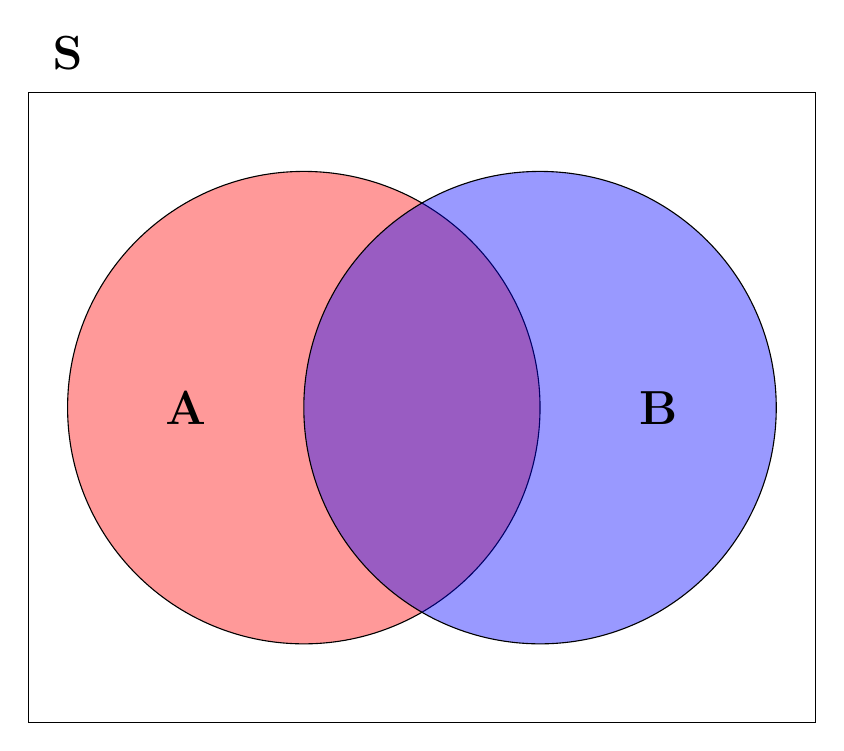
\begin{tikzpicture}
		%% You can adjust the opacity here. For venn diagrams it is convenient to have a low opacity so that you can see intersections
		\begin{scope} [fill opacity = .4]
			%% The draw command knows a lot of shapes. To make a rectangle you just need to specify two diagonal corners. Make sure you always have a semicolon at the end of your draw commands, otherwise latex flips out.
			\draw (-5,4) rectangle (5,-4);
			%% Similarly, you can make a circle by specifying the center and then the radius. You can also add a fill color, but if you're printing in black and white you'll probably want to remove that line.
			\draw[fill=red, draw = black] (-1.5,0) circle (3);
			\draw[fill=blue, draw = black] (1.5,0) circle (3);
			%% We can use the node command to label points. If you put your cursor on "LARGE" or "textbf" a box will drop down with size and text style options.
			\node at (-4.5,4.5) [text opacity = 1] {\LARGE\textbf{S}};
			\node at (-3,0) [text opacity = 1] {\LARGE\textbf{A}};
			\node at (3,0) [text opacity = 1] {\LARGE\textbf{B}};
		\end{scope}
		%% And now you have a venn diagram. Yay!
		%\draw[help lines](-5,5) grid (5,-6);    This line can draw the grid lines to help guide you. I use these when I'm writing the code and then delete this line when I publish the pdf.
	\end{tikzpicture}
	\caption{The purple area at the intersection of A and B is counted twice when naively adding the areas of A and B.} 
\end{figure} 

The probability of $ E \cup F $ is not the naive sum of the two individual probabilities, as seen in the Venn diagram here.

\begin{align}
	P(E \cup F) = P(E) + P(F) - P(E \cap F)
\end{align}

\textit{Odds} : the odds of an event is defined as a measure how much more likely an event is to occur compared to its complement. 

\begin{align}
	\frac{P(A)}{P(A^\complement)} = \frac{P(A)}{1 - P(A)}
\end{align}

\textbf{Equally likely outcomes} : It is common in real world experiments that every element of the sample space is equally likely. (Dice roll, coin flip, Lottery etc.). This special case simplifies the probability of an event to : 

\begin{align}
	P(E) = \frac{\text{number of element in E}}{\text{number of total elements}}
\end{align}

\textbf{Basic principles of counting} : For $ k $ repetitions of an experiment each with outcomes $ \{ n_1, n_2, ...., n_k \} $ respeectively, the total number of outcomes of the set of $ k $ repetitions is $ \left( \prod n_i  \right)$ 

\textit{Permutation} : The number of ways of selecting $ k $ out of $ n $ elements with sequence being relevant.

\begin{align}
	\Myperm{k} = \frac{n!}{(n-k)!} = \Mycomb{k} \ k! 
\end{align}

\textit{Combination} : The number of ways of selecting $ k $ out of $ n $ elements without regard to sequence. By convention, $ \Mycomb{0} = 1 $, using the fact that $ 0! = 1 $

\begin{align}
	\Mycomb{k} = \frac{n!}{(n-k)! \ k!} = \binom{n}{k}
\end{align}

\textbf{Conditional probability} : Useful when part of the outcome is known but not the full details. It looks at the probability of one event ($ A $) occurring, given another event ($ B $) has occurred. If the event $ B $ has occurred, then the sample space is now $ B $ instead of the initial $ S $. The desirable set of events now becomes the subset of elements in $ A $ that also happen to be in $ B $. This leads to the definition :

\begin{align}
	P(A|B) = \frac{P(A \cap B)}{P(B)}
\end{align}

Rearranging the above definition provides a convenient way to calculate the probability of the intersection of two events. 

\begin{align}
	P(A \cap B) = P(A|B)\ P(B)
\end{align}

\textbf{Bayes' theorem} : To find the probability of an event occurring, it is often useful to 'condition' it on the occurrence of another event. Using the definition of the complement of an event, 

\begin{align}
	P(A) &= P(A \cap B) + P(A \cap B^\complement) \\
	%
	P(A) &= P(A|B)\ P(B) + P(A|B^\complement)\ P(B^\complement)\\
	%
	P(A) &= P(B) \ P(A|B) + (1 - P(B))\ P(A|B^\complement)
\end{align}

Note that $ P(A) $ above becomes a linear interpolation between the two edges $ P(A|B) $ and $ P(A|B^\complement) $ with the sliding parameter being $ P(B) $. This is a useful perspective for many real-world problems.

An important pillar of Bayesian probability is the notion of updating a prior probability estimate after incorporating new (usually incomplete) information about the outcome.

The generalization of the conditional probability formula to more than two events is called Bayes' theorem. Let the set of mutually exclusive events $ \{ B_i \} $ be such that exactly one of them must occur.

\begin{align}
	\bigcup_{i = 1}^{n} B_i &= S \qquad \text{and} \qquad B_i \cap B_j = \varnothing \quad \forall \quad i \neq j \\
	%
	P(B_k|A) &= \frac{P(A \cap B_k)}{P(A)} = \frac{P(A | B_k) \ P(B_k)}{\sum_{i}P(A | B_i) \ P(B_i)}
\end{align}

The historical use of this formula was to update the probabilities of various hypotheses $ {B_i} $ after an experiment provides additional evidence $ A $.

\textbf{Independent events} : Two events are independent if the occurrence of one event does not affect the occurrence of the other event. 

\begin{align}
	P(A \cap B) &= P(A) \ P(B) \\
	%
	P(A|B) &= \frac{P(A \cap B)}{P(B)} = P(A)
\end{align}

If $ A $ and $ B $ are independent events, then so are $ A $ and $ B^\complement $. The above result extends to more than two events if any possible subset of the events is also independent. 

\newpage


%\include{./TeX_files/exercise03}
%\chapter{Random Variables and Expectation}


\begin{flushright}
	\textit{``Ch4 quote here"} 
\end{flushright}

\textbf{Random Variables} : Some result of an experiment that the experimenter is interested in observing. This may not necessarily be the full details of the experiment. Ex : number of heads observed when tossing 10 coins, without worrying about the outcomes of the individual coin-tosses themselves.

Conventionally denoted by uppercase letters. A random variable can either be discrete or continuous. It is constrained by the same normalization condition as any other set of events making up a sample space. For the simple case of an integer valued random variable which ranges from $ \left[1, n\right] $

\begin{align}
	P(S) = P \left( \bigcup_{i = 1}^{n}\left\{X = i\right\} \right) = \sum_{1}^{n} P \left\{X = i\right\} = 1
\end{align}

\textit{Indicator random variable} : acts a Boolean flag indicating whether or not an event happens. Usually takes on two discrete values, 0 or 1.

\textbf{Cumulative distribution function} : For a continuous random variable, it is possible to define a function that measures the probability that this random variable $ (X) $ is lesser than or equal to some real value $ (x) $.

\begin{align}
	F(x) = P \left\{ X \leq x \right\}
\end{align}

Shorthand notation $ F ~ X $ is used to denote the fact that $ F $ is the distribution function for the random variable $ X $. Using the monotonically increasing nature of $ F $, for some real numbers $ b \geq a $

\begin{align}
	P \left\{ a < X \leq b \right\} = F(b) - F(a)
\end{align}

\textbf{Probability Mass function} : For a discrete random variable, this attempts to assign a probability to each of the distinct possible outcomes. There is an implicit assumption that the discrete values are mutually exclusive outcomes. Let the random variable $ X $ take on one of the possible values $ \left\{x_i\right\} $

\begin{align}
	p(a) &= P \left\{X = a\right\} \\
	%
	p(x) &\geq 0 \quad \forall \quad x \in \left\{x_i\right\} \\
	%
	p(x) &= 0 \quad \text{otherwise}
\end{align}

The equivalent normalization condition for the probability mass distribution is : 
\begin{align}
	\sum\limits_{i = 1} p(x_i) = 1
\end{align}

\textit{Discrete cumulative distribution function} : The equivalent of the above CDF for the special case of discrete random variables is : 

\begin{align}
	F(a) = \sum\limits_{x \leq a} p(x_i)
\end{align}

Notice that a discrete probability mass function looks like a bar plot while the corresponding CDF looks like a step function with the vertical step size being $ p(x_i) $ at every $ x = x_i $.

\textbf{Probability density function} : The analog of the PMF for a continuous random variable, using the fact that integration is the generalized version of summation. Consider a continuous random variable $ X $, and a set of real numbers $ B $.

\begin{align}
	P \left\{X \in B \right\} = \int\limits_{x \in B} f(x) \ \mathrm{d}x
\end{align}

The normalization condition on a PDF is that the area under the PDF curve over the entire real line sums to $ 1 $. : 

\begin{align}
	P \left\{X \in \left(-\infty , \infty \right) \right\} = \int\limits_{-\infty}^{\infty} f(x) \ \mathrm{d}x = 1
\end{align}

Even though the probability that a continuous random variable will assume a particular discrete value is zero, it does have a finite probability of assuming a value in a finite-sized continuous set.

\begin{align}
	P \left\{X = a \right\} &= 0 \\
	%
	P \left\{ a \leq X \leq b \right\} &= \int\limits_{a}^{b} f(x) \ \mathrm{d}x
\end{align}

The above relation can be used to infer that the probability of a random variable $ X $ having a value in an interval of size $ \epsilon $ around $ a $ is given by $ \epsilon f(a) $, assuming $ \epsilon $ is sufficiently small. 

For a random variable $ X $, a PDF (denoted $ f $) leads to a CDF (denoted $ F $) using the above integration.
\begin{align}
	F(a) &= P \left\{ X \in \left( -\infty, a \right]  \right\} = \int\limits_{-\infty}^{a} f(x) \ \mathrm{d}x \\
	%
	f(a) &= \frac{\mathrm{d}}{\mathrm{d}a} F(a)
\end{align}

\textbf{Jointly distributed RVs} : Extending the above definitions to more than one dimension in order to observe the relationship between two or more random variables, gives the joint CDF

\begin{align}
	F(x, y) = P \left\{ X \leq a, Y \leq b \right\}
\end{align}

Notice that dimensional reduction of this joint CDF, in order to isolate the CDF of just one of the random variables is achieved by integrating over all possible values of the other variables.

\begin{align}
	F_X (x) &= P \left\{ X \leq x \right\} \nonumber \\
	%
	&= P \left\{ X \leq x, Y < \infty \right\} \nonumber \\
	%
	&= F(x, \infty)
\end{align}

The joint PMF for two discrete variables $ X, Y $ each taking on values in the sets $ \left\{ x_i \right\}, \left\{ y_j \right\} $ is given by

\begin{align}
	p(x_i, y_j) = P \left\{ X = x_i, Y = y_j \right\}
\end{align}

Isolating the PMF of one of the variables simply involves summing over the probabilities of all possible values of the other variables. This is called the \textit{marginal PMF} of one of the many variables. A joint PMF can always be used to find the individual PMFs, but not vice versa.

\begin{align}
	P \left\{ X = x_i \right\} &= P \left( \bigcup_{j} \left\{ X = x_i, Y = y_j \right\} \right)  \nonumber\\
	%
	&= \sum\limits_{j} P \left\{ X = x_i, Y = y_j \right\} \nonumber\\
	%
	&= \sum\limits_{j} P \left\{x_i,y_j \right\}
\end{align}

\textit{Jointly continuous RVs} : Extending the definitions of a CDF and PDF to more than one dimension enables the definition of a joint probability.

Consider two continuous RVs $ X, Y $ whose domains are the real sets $ A, B $ respectively. The two-dimensional real set $ C = \left\{ (x,y) \ :\ x \in A, y \in B  \right\} $ consists of ordered pairs of real numbers.

\begin{align}
	P \left\{ (X, Y) \in C \right\} &= \iint\limits_{(x, y) \in C} f(x,y)\ \mathrm{d}x \  \mathrm{d}y \\
	%
	P \left\{ X \in A, Y \in B \right\} &= \int\limits_{B} \int\limits_{A} f(x,y)\ \mathrm{d}x \  \mathrm{d}y
\end{align}

The CDF of two jointly distributed continuous RVs using the prior one-dimensional case is

\begin{align}
	F(a, b) &= P \left\{ X \in \left( -\infty, a \right],  Y \in \left( -\infty, b \right] \right\} \nonumber \\
	%
	&= \int\limits_{-\infty}^{a} \int\limits_{-\infty}^{b} f(x,y)\ \mathrm{d}x \  \mathrm{d}y \\
	%
	f(a, b) &= \frac{\partial^2}{\partial a\  \partial b} F(a, b)
\end{align}

Integrating over an infinitesimal 2-D space, $ ( f(a, b)\ \mathrm{d}a \ \mathrm{d}b )$ is a representation of how likely the random vector $ (X, Y) $ is to be located in a $ \mathrm{d}a \ \mathrm{d}b $ vicinity of the point $ (a, b) $.

The marginal PDF of one of the two jointly distributed continuous variables is found by integrating over all possible values of the other variable.

\begin{align}
	P \left\{ X \in A \right\} &= P \left\{ X \in A, Y \in \left( -\infty, \infty \right) \right\} \nonumber \\
	%
	&= \int\limits_{A} \int\limits_{-\infty}^{\infty} f(x,y)\ \mathrm{d}y \  \mathrm{d}x \nonumber \\
	%
	&= \int\limits_{A} f_X (x)\ \mathrm{d}x
\end{align}

The above simplification uses the marginal PDF 

\begin{align}
	f_X (x) = \int\limits_{-\infty}^{\infty} f(x,y)\ \mathrm{d}y \\
	%
	f_Y (y) = \int\limits_{-\infty}^{\infty} f(x,y)\ \mathrm{d}x
\end{align}

\textbf{Independent Random Variables} : If for any two sets of real numbers $ A, B$, and events $ E_A, F_B $ defined by $ \left\{ X \in A \right\},  \left\{ Y \in B \right\}$,

\begin{align}
	P \left\{ X \in A, Y \in B \right\} &= P \left\{ X \in A \right\} \ P \left\{ Y \in B \right\} \\
	%
	P(E_A F_B) &= P(E_A)\ P(F_B) \nonumber
\end{align}

then, the RVs $ X, Y$ are independent.

A similar condition holds for the joint CDF $ F(a, b) $ of two independent RVs $ X, Y $

\begin{align}
	P \left\{ X \leq a, Y \leq b \right\} &= P \left\{ X \leq a \right\} \ P \left\{ Y \leq b \right\}  \nonumber \\
	%
	F(a, b) &= F_X(a)\ F_Y(b) \qquad \forall \qquad a, b
\end{align}

The condition for independence states that knowing the value of one RV does not change the distribution of another.The joint PMF of two independent discrete RVs also follows a similar constraint.

\begin{align}
	p(x, y) &= p_X(x)\ p_Y(y) \qquad \forall \qquad x, y
\end{align}

For continuous independent RVs, the correspoding constraint on their joint PDF is

\begin{align}
	f(x, y) &= f_X(x)\ f_Y(y) \qquad \forall \qquad x, y
\end{align}

For the generalized case of $ n $ independent RVs, the entire set of RVs is independent only if all possible subsets of these RVs are also independent.

\textbf{Conditional distributions} : Using the definition of conditional probability of two events, the conditional PMF for two RVs $ X, Y $ is defined as 

\begin{align}
	p_{X|Y}(x\ |\ y) &= P \left\{ X = x\ |\ Y = y \right\} \nonumber\\
	%
	&= \frac{P \left\{ X = x, Y = y \right\}}{P \left\{ Y = y \right\}} \nonumber\\
	%
	&= \frac{p(x, y)}{p_Y(y)}
\end{align}

The conditional PDF of two continuous RVs $ X, Y $ indicates the probability that $ X $ is in the vicinity of $ x $, given that $ Y $ is in the vicinity of $ y $.

\begin{align}
	f_{X|Y}(x\ |\ y) &= \frac{f(x, y)}{f_Y(y)} \\
	%
	P(X \in A\ |\ Y = y) &= \int\limits_{A} f_{X|Y}(x\ |\ y) \ \mathrm{d} x
\end{align}

\textbf{Expected value} : The expectation of a random variable $ X $, is simply the average value of that random variable weighted by the probabilities of each possible value. $ \mathbb{E}[X] $ need not be a value that $ X $ can actually take. It has the same units of measurement as $ X $ itself.

\begin{align}
	\mathbb{E}[X] = \sum\limits_{i} x_i\ P \left\{ X = x_i \right\} 
\end{align}

If $ I $ is an indicator RV for the event $ A $, then 

\begin{align}
	\mathbb{E}[I] = 1 \times P(A) + 0 \times P(A^\complement) = P(A)
\end{align}

\textit{Entropy} : A system of measuring the expected amount of information conveyed by a RV which can take on of $ n $ different values. This is measured in bits.

\begin{align}
	H(X) = -\sum\limits_{i = 1}^{n} p_i \ \log_{2}(p_i)
\end{align}

Here, the information conveyed by each possible value of the RV is summed using the probabilities as weights.

\begin{align}
	I\left\{X = x_i\right\} &= -\log_{2}(p_i) \\
	%
	H(X) &= \sum\limits_{i = 1}^{n} p_i \ I\left\{X = x_i\right\}
\end{align}

The expectation value of a continuous RV (analogous to the definition of the center of mass of a continuous object) is

\begin{align}
	\mathbb{E}[X] = \int_{-\infty}^{\infty} x\ f(x)\ \mathrm{d}x
\end{align}

\textbf{Properties of expected value} : With a known PDF for a random variable $ X $, there are two approaches to finding the expected value of some function of $ X $.

$ \mathbb{E}[G(X)] = \mathbb{E}[Y] $ uses the substitution $ Y = G(X) $ to find the values taken by this new RV $ Y $ and then apply the weighted sum method.

For the less trivial case of a continuous RV $ X $, an existing PDF $ f_X (x) $ can be used to find the CDF $ F_Y(a) $ and then differentiated to produce the new PDF $ f_Y(a) $. The integral formula for $ \mathbb{E}[Y] $ is then easily applied. A more straightforward method is as follows, 

\begin{align}
	\mathbb{E}[g(X)] &= \sum\limits_{x} g(x)\ p(x)  \qquad \text{for discrete RV} \\
	%
	\mathbb{E}[g(X)] &= \int\limits_{x} g(x)\ f(x)\ \mathrm{d}x  \qquad \text{for continuous RV} \\
	%
	\mathbb{E}[aX + b] &= a \mathbb{E}[X] + b \nonumber
\end{align}

\textbf{Moments} : The expectation value generalized to higher powers is defined as the moment. The special case of $ n = 1 $ is merely the expected value.

\begin{align}
	\mathbb{E}[X^n] &= \sum_{x} x^n\ p(x) \qquad \text{for discrete RV} \\
	%
	\mathbb{E}[X^n] &= \int_{-\infty}^{\infty} x^n\ f(x)\ \mathrm{d}x \qquad \text{for continuous RV}
\end{align}

Generalizing to more than two RVs $ X, Y $ along with a function $ g(x,y) $ of two variables,

\begin{align}
	\mathbb{E}[g(X, Y)] &= \sum\limits_{x} \sum\limits_{y} g(x, y)\ p(x, y)  \qquad \text{for discrete RV} \\
	%
	\mathbb{E}[g(X, Y)] &= \int\limits_{-\infty}^{\infty} \int\limits_{-\infty}^{\infty} g(x, y)\ f(x, y)\ \mathrm{d}x \ \mathrm{d}y  \qquad \text{for continuous RV} \\
	%
	\mathbb{E}[X + Y] &= \mathbb{E}[X] + \mathbb{E}[Y] \nonumber
\end{align}

\textit{Mean value as an RV predictor} : Let the RV $ X $ with mean $ \mu $ be predicted to have a value $ c $ by an experimenter. From the point of view of minimizing the average squared error, the best prediction of the RV outcome is its mean.

\begin{align}
	\mathbb{E}[(X - c)^2] &= \mathbb{E}[(X - \mu)^2] + (\mu - c)^2 \nonumber \\
	%
	&\geq \mathbb{E}[(X - \mu)^2] 
\end{align}

\textbf{Variance} : The conventional measure of the spread in the values of a random variable, denoted by $ \mathrm{Var}(X) $. This is used alongside the expected value $ \mathbb{E}[X] $ to summarize the RV.

\begin{align}
	\mathrm{Var}(X) &= \mathbb{E}[(X - \mu)^2] \\
	%
	\mathrm{Var}(X) &= \mathbb{E}[X^2] - (\mathbb{E}[X])^2
\end{align}

For an indicator RV $ I $, which is a binary $ \left\{0, 1\right\} $ switch indicating the occurrence of event $ A $, the variance is 

\begin{align}
	\mathrm{Var}(I) &= P(A) [1 - P(A)]
\end{align}

The variance transforms using the following relation upon change of RV, 
\begin{align}
	\mathrm{Var}(aX + b) &= a^2 \ \mathrm{Var}(X) \\
	%
	\mathrm{Var}(b) &= 0 \\
	%
	\mathrm{Var}(X + b) &= \mathrm{Var}(X)
\end{align}

\textit{Standard Deviation} : defined as the square root of the variance, measured in the same units as the underlying RV. 
\begin{align}
	s_X = \sqrt{\mathrm{Var}(X)}
\end{align}

\textbf{Covariance} : $ \mathrm{Var}(X + Y) \neq \mathrm{Var}(X) + \mathrm{Var}(Y) $ except for the special case of $ X, Y $ being independent RVs. Consider the two RVs $ X, Y $ with means $ \mu_x , \mu_y$ respectively.

\begin{align}
	\mathrm{Cov}(X, Y) &= \mathbb{E}[(X - \mu_x)(Y - \mu_y)] \\
	%
	\mathrm{Cov}(X, Y) &= \mathbb{E}[XY] - \mathbb{E}[X] \ \mathbb{E}[Y]
\end{align}

Covariance has the following useful properties, 

\begin{align}
	\mathrm{Cov}(X, Y) &= \mathrm{Cov}(Y, X) \\
	%
	\mathrm{Cov}(X, X) &= \mathrm{Var}(X) \\
	%
	\mathrm{Cov}(aX, Y) &= a \ \mathrm{Cov}(X, Y) \\
	%
	\mathrm{Cov}(X_1 + X_2, Y) &= \mathrm{Cov}(X_1, Y) + \mathrm{Cov}(X_2, Y)
\end{align}

Generalizing the above relation to two sets of RVs $ \left\{X_i\right\}, \left\{Y_j\right\} $ gives the following relation, 
\begin{align}
	\mathrm{Cov} \left( \sum\limits_{i}X_i , \sum\limits_{j}Y_j \right) = \sum\limits_{i} \sum\limits_{j} \mathrm{Cov} (X_i, Y_j)
\end{align}

Replacing the $ \left\{Y_j\right\} $ set of RVs with another copy of the first set $  \left\{X_i\right\} $ in the above relation, gives a formula for the variance of the sum of RVs.

\begin{align}
	\mathrm{Var} \left( \sum\limits_{i}X_i \right) = \sum\limits_{i} \mathrm{Var}(X_i) + \sum\limits_{i} \sum\limits_{j \neq i} \mathrm{Cov} (X_i, X_j)
\end{align}

For the special case of independent RVs $ X, Y $, and thus for a set of independent RVs $ \left\{X_i\right\} $

\begin{align}
	\mathrm{Cov}(X, Y) &= 0 \\
	%
	\mathrm{Var} \left( \sum\limits_{i}X_i \right) &= \sum\limits_{i}\mathrm{Var}(X_i) 
\end{align}

\textbf{Correlation} : Normalizing the covariance of two RVs by the product of their standard deviations results in a quantity $ \mathrm{Corr}(X, Y) $ which lies in the range $ \left[-1, 1\right] $. A positive correlation shows that an increase in $ X $ tends to be accompanied by an increase in $ Y $ and vice versa.

\begin{align}
	\mathrm{Corr}(X, Y) = \frac{\mathrm{Cov}(X, Y)}{s_x s_y}
\end{align}

Consider two indicator RVs $ X, Y $ for two underlying events $ A, B $. Now, the correlation measures the increase in probability of occurrence of $ A $ given the occurrence of $ B $. 

\begin{align}
	\mathrm{Corr}(X, Y) &> 0  \qquad \Leftrightarrow \qquad P \left\{ Y = 1\ |\ X = 1 \right\} > P \left\{ Y = 1 \right\}
\end{align}

\textbf{Moment generating functions} : A function which gives all of the moments of a RV $ X $, upon repeated differentiation. This is defined for all values of the parameter $ t $.

\begin{align}
	\phi(t) &= \mathbb{E}[e^{tX}] \\
	%
	\phi(t) &= \sum_{x} e^{tx} \ p(x) \qquad \text{for discrete RV} \\
	%
	\phi(t) &= \int_{-\infty}^{\infty} e^{tx}\ f(x)\ \mathrm{d}x \qquad \text{for continuous RV} 
\end{align}

Some useful properties of the function $ \phi(t) $ when evaluated at $ t = 0 $,

\begin{align}
	\phi^n (0) &= \mathbb{E}[X^n] \qquad n \geq 1 \\
	%
	\phi'(0) &= \mathbb{E}[X] \qquad \text{is the mean} \\
	%
	\phi''(0) - \left(\phi'(0)\right)^2 &= \mathrm{Var}(X) \qquad \text{is the variance}
\end{align}

The moment generating function corresponds one-to-one with the distribution function of a given RV. Also, for the special case of two independent RVs $ X, Y $

\begin{align}
	\phi_{X + Y}(t) = 	\phi_{X}(t)\ \phi_{X}(t)
\end{align}

\textbf{Markov's inequality} : For a random variable $ X $, that only takes non-negative values, and some $ a > 0 $,
\begin{align}
	P\left\{ X \geq a \right\} \leq \frac{\mathbb{E}[X]}{a}
\end{align}

\textbf{Chebyshev's inequality} : Using $ a = k^2 $ and the non-negative RV $\left| X - \mu \right|$,
\begin{align}
	P\left\{( X - \mu)^2 \geq k^2 \right\} &\leq \frac{\mathbb{E}[(X - \mu)^2]}{k^2} \nonumber \\
	%
	P\left\{\left| X - \mu \right| \geq k\right\} &\leq \frac{\sigma^2}{k^2} \nonumber \\
	%
	P\left\{\left| X - \mu \right| \geq n\sigma \right\} &\leq \frac{1}{n^2}
\end{align}

The above inequalities help derive bounds on probabilities when only the mean and/or variance of the distribution is known.

\textbf{Weak Law of large numbers} : Consider a set of independent, identically distributed random variables $ \left\{X_i\right\} $, each with the same mean. $ \mathbb{E}[X_i] = \mu $, and $ \epsilon > 0 $.

\begin{align}
	P \left\{ \left| \frac{ X_1 + X_2 + \dots + X_n }{n} - \mu \right|\  >\ \epsilon \right\} \to 0 \qquad
	\text{as } x \to \infty
\end{align}

The mean of the first $ n $ experimental outcomes measuring the RV $ X $ is a distance $ \epsilon $ away from the true expected value $ \mu $. This distance approaches $ 0 $ as $ n $ approaches $ \infty $.

A restatement of the above uses the experiment of sampling a fixed distribution $ n $ times and measuring the distance between the sample mean and the true mean. As the number of samples increases, the sample mean approaches the true mean asymptotically.
\newpage
%\chapter*{Exercises C4}

\begin{enumerate}
	\item $ \left\{X = 1 \right\}$ requires a woman in first place. This involves selecting one of five women to fill first place and then arranging the rest of the 9 people. Alternatively, consider the fact that half of all possible arrangements will have a woman in first place.\\
	\begin{align}
		P \left\{X = 1 \right\} &= \frac{\Mycomb[5]{1} \times \Mycomb[9]{5} \ 5! \times 4!}{\Mycomb[10]{5} \ 5! \times 5!} = \frac{\Mycomb[9]{4}}{\Mycomb[10]{5}} = \frac{1}{2} \nonumber \\
		%
		P \left\{X = 2 \right\} &= \frac{\Mycomb[5]{1} \times \Mycomb[5]{1} \times \Mycomb[8]{4}\ 4! \times 4!}{\Mycomb[10]{5} \ 5! \times 5!} = \frac{\Mycomb[8]{4}}{\Mycomb[10]{5}} = \frac{25}{90} \nonumber \\
		%
		P \left\{X = 3 \right\} &= \frac{\Mycomb[5]{2}\ 2! \times \Mycomb[5]{1} \times \Mycomb[7]{4}\ 4! \times 3!}{\Mycomb[10]{5} \ 5! \times 5!} = \frac{\Mycomb[7]{4}}{\Mycomb[10]{5}} = \frac{100}{720}
	\end{align}\\
	
	Clearly, the trend indicates that \\
	$ P \left\{X = 4 \right\}  = \Mycomb[6]{4} / \Mycomb[10]{5} = 15/252$, \\
	$ P \left\{X = 5 \right\}  = \Mycomb[5]{4} / \Mycomb[10]{5} = 5/252$, \\
	$ P \left\{X = 6 \right\}  = \Mycomb[4]{4} / \Mycomb[10]{5} = 1/252$. This is the greatest possible value that $ X $ can take, as there are only five men. \\
	
	\item The extreme cases are $ n $ heads and $ n $ tails. So , \\
	$ X \in \left\{-n, -(n-2), \dots, \dots, (n-2), n \right\} $. This set contains $ 0 $ if $ n $ is even. This assumes that the difference is not an absolute value. \\
	
	\item \begin{align}
		P \left\{X = 3 \right\} &= P \left\{X = -3 \right\} = \frac{1}{2^3} = \frac{1}{8} \nonumber \\
		%
		P \left\{X = 1 \right\} &= P \left\{X = -1 \right\} = \frac{3}{2^3} = \frac{3}{8}
	\end{align}\\
	
	\item \begin{enumerate}
		
		\item The PDF is plotted as follows : 	
		\begin{figure}[H]
			\centering
			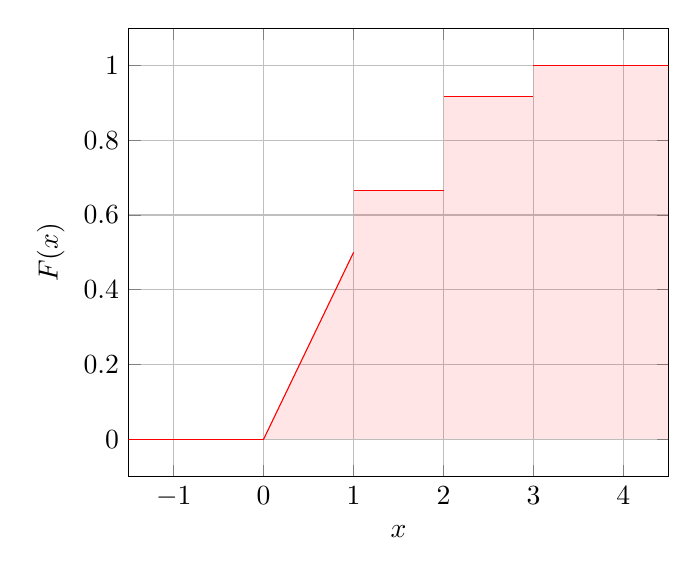
\begin{tikzpicture}
				\begin{axis}[xlabel=$x$, grid = both, ylabel = $F(x)$, xmin = -1.5, xmax = 4.5]
					\addplot[draw=red][name path = f1, domain = -2:0]{0};
					\addplot[draw=red][name path = f2, domain = 0:1]{x/2};
					\addplot[draw=red][name path = f3, domain = 1:2]{2/3};
					\addplot[draw=red][name path = f4, domain = 2:3]{11/12};
					\addplot[draw=red][name path = f5, domain = 3:5]{1};
					
					\path[name path=axis1] (axis cs:-2,0) -- (axis cs:0,0);
					\path[name path=axis2] (axis cs:0,0) -- (axis cs:1,0);
					\path[name path=axis3] (axis cs:1,0) -- (axis cs:2,0);
					\path[name path=axis4] (axis cs:2,0) -- (axis cs:3,0);
					\path[name path=axis5] (axis cs:3,0) -- (axis cs:5,0);
					
					\addplot [thick,color=red,fill=red, fill opacity=0.1] fill between[of=f1 and axis1,];
					\addplot [thick,color=red,fill=red, fill opacity=0.1] fill between[of=f2 and axis2,];
					\addplot [thick,color=red,fill=red, fill opacity=0.1] fill between[of=f3 and axis3,];
					\addplot [thick,color=red,fill=red, fill opacity=0.1] fill between[of=f4 and axis4,];
					\addplot [thick,color=red,fill=red, fill opacity=0.1] fill between[of=f5 and axis5,];
				\end{axis}
			\end{tikzpicture}
		\end{figure}
		
		\item $ P \left\{X > 1/2\right\} = 1 - F(1/2) $, from the plot above, this is $ 3/4 $ \\
		
		\item $ P \left\{ 2 < X \leq 4 \right\} = F(4) - F(2) = 1/12 $ \\
		
		\item $ P \left\{ X < 3 \right\} = F(4) - F(2) = 11/12 $ when asymptotically approaching $ x = 3 $ from the left. \\
		
		\item  \begin{align}
			P \left\{ X = 1 \right\} = F(1) - \lim\limits_{x \to 1^-} F(x) = \frac{2}{3} - \frac{1}{2} = \frac{1}{6} \nonumber
		\end{align}\\
		
	\end{enumerate}
	
	\item 
	\begin{subequations}
		\begin{enumerate}
			\item \begin{align}
				\int\limits_{-\infty}^{\infty} f(x)\ \mathrm{d}x &= 1 \nonumber \\
				%
				\int\limits_{0}^{1} c x^3\ \mathrm{d}x &= 1 \nonumber\\
				%
				\frac{c}{4}\ (x^4) \Big|_0^1 &= 1 \qquad \to \qquad c = 4
			\end{align} \\
			
			\item \begin{align}
				P \left\{0.4 < X < 0.8 \right\} = \int\limits_{0.4}^{0.8} 4 x^3\ \mathrm{d}x = 0.384
			\end{align}\\
		\end{enumerate}
	\end{subequations}
	
	\item normalization constraint demands \\
	\begin{subequations}
		\begin{align}
			\int\limits_{-\infty}^{\infty} f(x)\ \mathrm{d}x &= 1 \nonumber \\
			%
			\int\limits_{0}^{\infty} \lambda \exp(-0.01x)\ \mathrm{d}x &= 1 \nonumber\\
			%
			-100 \lambda \ \exp(-0.01x) \Big|_0^\infty &= 1 \qquad \to \qquad \lambda = \frac{1}{100} \\
			%
			P \left\{50 < X < 150 \right\} &= \int\limits_{50}^{150}\ 0.01\ \exp(-0.01x)\ \mathrm{d}x \nonumber \\
			%
			&= \exp(-0.01x)\ \Big|_{150}^{50} = 0.3834 \\
			%\int\limits_{0}^{\infty} \lambda \exp(-0.01x)\ \mathrm{d}x &= 1 \nonumber\\
			%
			P \left\{X < 100 \right\} &= \int\limits_{0}^{100}\ 0.01\ \exp(-0.01x)\ \mathrm{d}x \nonumber \\
			%
			&= \exp(-0.01x)\ \Big|_{100}^{0} = 0.6321
		\end{align}\\
	\end{subequations}
	
	\item Let E be the event that a radio set fails within 150 hours. $ E = \left\{ X < 150 \right\} $ \\
	\begin{subequations}
		\begin{align}
			P(E) &= \int\limits_{-\infty}^{150} f(x) \ \mathrm{d}x \nonumber\\
			%
			&= \int\limits_{100}^{150} \frac{100}{x^2} \ \mathrm{d}x \nonumber\\
			%
			&= \frac{100}{x}\ \Big|_{150}^{100} = \frac{1}{3} \\
			%
			P(\text{exactly 3 fail}) &= \Mycomb[5]{2} \ (P(E))^2 (1 - P(E))^3 = \frac{10 \times 8}{243} = 0.33
		\end{align}\\
	\end{subequations}
	
	\item normalization constraint demands \\
	\begin{subequations}
		\begin{align}
			\int\limits_{-\infty}^{\infty} f(x)\ \mathrm{d}x &= 1 \nonumber \\
			%
			\int\limits_{0}^{\infty} c \ \exp(-2x)\ \mathrm{d}x &= 1 \nonumber\\
			%
			-\frac{c}{2} \ \exp(-2x) \Big|_0^\infty &= 1 \qquad \to \qquad c = 2 \\
			%
			P \left\{X > 2 \right\} &= \int\limits_{2}^{\infty}\ 2\ \exp(-2x)\ \mathrm{d}x \nonumber \\
			%
			&= \exp(-2x)\ \Big|_{\infty}^{2} = 0.0183
		\end{align}\\
	\end{subequations}
	
	\item joint PMF of $ N_1, N_2 $, given 3 out of 5 are defective. $ N_1 \in \left\{1, 2, 3\right\} $ and $ N_2 \in \left\{ 1, 2, 3 \right\} $. Using the notation $ P(N_1, N_2) $\\
	
	\begin{align}
		P(1, 1) = \frac{\Mycomb[3]{1}}{\Mycomb[5]{3}} = \frac{3}{10} \nonumber \\
		%
		P(1, 2) = \frac{\Mycomb[2]{1}}{\Mycomb[5]{3}} = \frac{2}{10} \nonumber \\
		%
		P(1, 3) = \frac{\Mycomb[1]{1}}{\Mycomb[5]{3}} = \frac{1}{10} \nonumber \\
		%
		P(2, 1) = \frac{\Mycomb[2]{1}}{\Mycomb[5]{3}} = \frac{2}{10} \nonumber \\
		%
		P(2, 2) = \frac{\Mycomb[1]{1}}{\Mycomb[5]{3}} = \frac{1}{10} \nonumber \\
		%
		P(3, 1) = \frac{\Mycomb[1]{1}}{\Mycomb[5]{3}} = \frac{1}{10} \nonumber \\
	\end{align} \\
	
	\item 
	\begin{enumerate}
		\begin{subequations}
			\item 
			normalization constraint demands \\
			\begin{align}
				\int\limits_{0}^{2} \int\limits_{0}^{1} f(x, y)\ \mathrm{d}x \ \mathrm{d}y &= P(S) \nonumber \\
				%
				\int\limits_{0}^{2} \int\limits_{0}^{1} \frac{6x^2}{7} + \frac{3xy}{7}\ \mathrm{d}x \ \mathrm{d}y &= P(S) \nonumber\\
				%
				\int\limits_{0}^{2} \left(\frac{2x^3}{7} \Big|_0^1 + y \times \frac{3x^2}{14} \Big|_0^1  \right) \ \mathrm{d}y &= P(S) \nonumber \\
				%
				\int\limits_{0}^{2} \frac{3y + 4}{14}\ \mathrm{d}y &= P(S) \nonumber \\
				%
				\frac{3y^2 + 8y}{28} \Big|_0^2 &= P(S) = 1
			\end{align}\\
			
			\item to find the marginal PDF of $ X $, \\
			\begin{align}
				f_X (x) &= \int\limits_{0}^{2} f(x, y)\ \mathrm{d}y \nonumber \\
				%
				&= \left( \frac{6x^2}{7} \times y \Big|_0^2 + \frac{3x}{14} \times y^2 \Big|_0^2  \right) \nonumber \\
				%
				&= \frac{12x^2 + 6x}{7}
			\end{align}
			
			\item to find $ P \left\{ X > Y \right\} $\\
			
			\begin{align}
				P\left\{ X > Y\right\} &= \int\limits_{0}^{1} \int\limits_{y}^{1} f(x, y)\ \mathrm{d}x \ \mathrm{d}y \nonumber \\
				%
				&= \int\limits_{0}^{1} \left(\frac{2x^3}{7} \Big|_y^1 + y \times \frac{3x^2}{14} \Big|_y^1  \right) \ \mathrm{d}y  \nonumber \\
				%
				&= \int\limits_{0}^{1} \frac{4 - 4y^3 + 3y - 3y^3}{14} \ \mathrm{d}y  \nonumber \\
				%
				&= \frac{1}{14} \left( 4y + \frac{3y^2}{2} - \frac{7y^4}{4} \right)\Big|_0^1 \ \mathrm{d}y  = \frac{15}{56}
			\end{align}\\
			
		\end{subequations}
	\end{enumerate}
	
	\item to find the CDF, find the probability that none of the RVs are larger than $ M $. Given the RVs are independent, \\
	
	\begin{subequations}
		\begin{align}
			P\left\{X_i \leq x \right\} &= \frac{x}{1} = x \nonumber \\
			%
			F_M (x) &= P\left\{M \leq x\right\} = P\left\{X_1 \leq x, \dots , X_n \leq x\right\} \nonumber \\
			%
			F_M (x) &= \prod_{i = 1}^{n} x = x^n \qquad \text{for} \qquad x \in \left[0, 1\right] \\
			%
			f_M (x) & = \frac{\mathrm{d}}{\mathrm{d} x} F(x) = nx^{n-1} \qquad x \in \left[0, 1\right]
		\end{align}\\
	\end{subequations}
	
	\item \begin{subequations}
		\begin{enumerate}
			\item To compute the marginal PDF of $ X $, 
			\begin{align}
				f_X (x) &= \int\limits_{0}^{\infty} f(x, y)\ \mathrm{d}y \nonumber \\
				%
				&= x e^{-x} \int\limits_{0}^{\infty} e^{-y}\ \mathrm{d}y \nonumber \\
				%
				&= x e^{-x} \left(e^{-y}\Big|_\infty^0\right) = x e^{-x}
			\end{align}\\
			
			\item To compute the marginal PDF of $ y $, 
			\begin{align}
				f_Y (y) &= \int\limits_{0}^{\infty} f(x, y)\ \mathrm{d}x \nonumber \\
				%
				&= e^{-y} \int\limits_{0}^{\infty} x\ e^{-x}\ \mathrm{d}x \nonumber \\
				%
				&= e^{-y} \left(xe^{-x}\Big|_\infty^0 + \int\limits_{0}^{\infty} e^{-x} \ \mathrm{d}x\right) = e^{-y}
			\end{align}\\
			
			\item $ f_X (x) \times f_Y (y)  = x e^{-(x + y)}$, which is equal to the joint PDF. Hence, $ X, Y $ are independent. \\
		\end{enumerate}
	\end{subequations}
	
	\item \begin{subequations}
		\begin{enumerate}
			\item To compute the marginal PDF of $ X $, 
			\begin{align}
				f_X (x) &= \int\limits_{0}^{\infty} f(x, y)\ \mathrm{d}y \nonumber \\
				%
				&= x e^{-x} \int\limits_{0}^{\infty} e^{-y}\ \mathrm{d}y \nonumber \\
				%
				&= x e^{-x} \left(e^{-y}\Big|_\infty^0\right) = x e^{-x}
			\end{align}\\
			
			\item To compute the marginal PDF of $ y $, 
			\begin{align}
				f_Y (y) &= \int\limits_{0}^{y} f(x, y)\ \mathrm{d}x \nonumber \\
				%
				&= \int\limits_{0}^{y} 2\ \mathrm{d}x = 2y  \qquad y \in (0, 1) \\
				%
				f_X (x) &= \int\limits_{x}^{1} f(x, y)\ \mathrm{d}y \nonumber \\
				%
				&= \int\limits_{x}^{1} 2\ \mathrm{d}y  = 2(1 - x)  \qquad x \in (0, 1)
			\end{align}\\
			
			\item $ f_X (x) \times f_Y (y)  = 4y(1-x)$, which is not equal to the joint PDF. Hence, $ X, Y $ are not independent. \\
		\end{enumerate}
	\end{subequations}
	
	\item  \begin{subequations}
		To compute the marginal PDF of $ X $ and $ Y $ separately, 
		\begin{align}
			f_X (x) &= \int\limits_{-\infty}^{\infty} f(x, y)\ \mathrm{d}y \nonumber \\
			%
			&= k(x) \int\limits_{-\infty}^{\infty} h(y)\ \mathrm{d}y \\
			%
			f_Y (y) &= \int\limits_{-\infty}^{\infty} f(x, y)\ \mathrm{d}x \nonumber \\
			%
			&= h(y) \int\limits_{-\infty}^{\infty} k(x)\ \mathrm{d}x
		\end{align}\\
		
		To check whether $ X, Y $ are independent, \\
		\begin{align}
			f_X (x) \times f_Y (y) &= h(y) \ k(x) \ \int\limits_{-\infty}^{\infty} k(x)\ \mathrm{d}x \ \int\limits_{-\infty}^{\infty} h(y)\ \mathrm{d}y \nonumber \\
			%
			&= h(y) \ k(x)\ \int\limits_{-\infty}^{\infty} \int\limits_{-\infty}^{\infty} h(y) k(x) \ \mathrm{d}x \ \mathrm{d}y  \nonumber \\
			%
			&= k(x)\ h(y) = f(x, y)
		\end{align} \\
		Hence, $ X, Y $ are independent. In the relation above, the integral of $ f(x, y) $ over the full domains of $ X, Y $ was 1 from the normalization condition. \\
	\end{subequations}
	
	\item The previous problems do obey the factoring rule. \\
	
	\item \begin{subequations}
		\begin{enumerate}
			\item \begin{align}
				P \left\{X + Y \leq a \right\} &= P \left\{ X \leq a - Y \right\} \nonumber \\
				%
				&= \int\limits_{-\infty}^{\infty} \int\limits_{-\infty}^{a - y} f_Y (y) \ f_X(x) \ \mathrm{d}x \ \mathrm{d}y  \nonumber \\
				%
				&= \int\limits_{-\infty}^{\infty} f_Y (y) \ F_X(a - y) \ \mathrm{d}y 
			\end{align}
			
			\item \begin{align}
				P \left\{ X \leq Y \right\} &= \int\limits_{-\infty}^{\infty} \int\limits_{-\infty}^{y} f_Y (y) \ f_X(x) \ \mathrm{d}x \ \mathrm{d}y  \nonumber \\
				%
				&= \int\limits_{-\infty}^{\infty} f_Y (y) \ F_X(y) \ \mathrm{d}y 
			\end{align}
		\end{enumerate}
	\end{subequations}
	
	\item To find the PDF, first find the CDF and then differentiate it. Note that the integral over current is split into two parts, one with constraint on resistance and other without. \\
	\begin{subequations}
		\begin{align}
			P \left\{ W \leq a \right\} &= F_W (a) \nonumber \\
			%
			&= \int\limits_{0}^{\sqrt{a}} \int\limits_{0}^{1}  f_R (y) \ f_I(x) \ \mathrm{d}x \ \mathrm{d}y  + \int\limits_{\sqrt{a}}^{1} \int\limits_{0}^{a/x^2}  f_R (y) \ f_I(x) \ \mathrm{d}x \ \mathrm{d}y \nonumber \\
			%
			&= \int\limits_{0}^{\sqrt{a}}  6x(1-x) \ \mathrm{d}x + \int\limits_{\sqrt{a}}^{1} \frac{a^2\ 6x(1-x)}{x^4} \ \mathrm{d}x \nonumber \\
			%
			&= \left(3x^2 - 2x^3\right) \Big|_0^{\sqrt{a}} + 6a^2\ \left(\frac{-2}{x^2} + \frac{1}{x}\right)\Big|_{\sqrt{a}}^{1} \nonumber \\
			%
			&= 3a - 2a^{3/2} - 6a^2 + 12a -6a^{3/2} \nonumber \\
			%
			&= - 6a^2 - 8a^{3/2} + 15a \\
			%
			f_W (a) &= \frac{\mathrm{d}}{\mathrm{d} a} F_W (a) = -12a - 12a^{1/2} + 15
		\end{align} \\
	\end{subequations}
	
	\item to determine $ P \left\{B\ |\ G = 2\right\} $. Also, define $ T = G+B $ \\
	\begin{subequations}
		\begin{align}
			P \left\{G = 2\right\} &= P \left\{G = 2\ |\ T = 0\right\}P \left\{T = 0\right\} \nonumber \\
			%
			&+ P \left\{G = 2\ |\ T = 1\right\}P \left\{T = 1\right\} \nonumber \\ 
			%
			&+ P \left\{G = 2\ |\ T = 2\right\}P \left\{T = 2\right\} \nonumber \\
			%
			&+ P \left\{G = 2\ |\ T = 3\right\}P \left\{T = 3\right\} \nonumber \\
			%
			&= 0 \times 0.15 + 0 \times 0.2 + \frac{1}{4} \times 0.35 + \frac{1}{8} \times 0.3 \nonumber \\
			%
			&= \frac{1}{8} \\
			%
			P \left\{B = 0\ |\ G = 2\right\} &= \frac{P \left\{B = 0, G = 2\right\}}{P \left\{G = 2\right\}} = \frac{1/4 \times 0.35}{1/8} = \frac{7}{10} \\
			%
			P \left\{B = 1\ |\ G = 2\right\} &= \frac{P \left\{B = 1, G = 2\right\}}{P \left\{G = 2\right\}} = \frac{1/8 \times 0.3}{1/8} = \frac{3}{10}
		\end{align} \\
	\end{subequations}
	
	\item to find the conditional PDF, \\
	\begin{subequations}
		\begin{enumerate}
			\item From problem 10 \\
			\begin{align}
				f_{X|Y}(x\ |\ y) &= P \left\{ X = x\ |\ Y = y \right\} = \frac{f(x, y)}{f_Y(y)}\nonumber\\
				%			
				f_Y (y) &= \int\limits_{0}^{1} f(x, y)\ \mathrm{d}x \nonumber \\
				%
				&= \left( \frac{2x^3}{7} \Big|_0^1 + 3y \times \frac{x^2}{14}\Big|_0^1  \right) \nonumber \\
				%
				&= \frac{4 + 3y}{14} \\
				%
				f_{X|Y}(x\ |\ y) &= \frac{12x^2 + 6xy}{3y + 4} \qquad x \in \left(0, 1\right)
			\end{align} \\
			
			\item From problem 13 \\
			\begin{align}
				f_{X|Y}(x\ |\ y) &= P \left\{ X = x\ |\ Y = y \right\} = \frac{f(x, y)}{f_Y(y)}\nonumber\\
				%			
				f_{X|Y}(x\ |\ y) &= \frac{2}{2(1-x)} = \frac{1}{1-x} \qquad x \in \left(0, 1\right)
			\end{align} \\
		\end{enumerate}
	\end{subequations}
	
	\item 
	\begin{subequations}
		\begin{enumerate}
			\item Assuming $ f_Y (y) $ is well defined in the domain of interest,
			\begin{align}
				f_{X|Y}(x\ |\ y) &= P \left\{ X = x\ |\ Y = y \right\} = \frac{f(x, y)}{f_Y(y)} \nonumber\\
				%
				f(x,y) &= f_X (x) \times f_Y (y) \quad \leftrightarrow \quad \text{X, Y are independent}  \nonumber\\
				%
				f_{X|Y}(x\ |\ y) &= f_X (x) \quad \leftrightarrow \quad \text{X, Y are independent}
			\end{align} \\
			
			\item Exactly same steps as the above
		\end{enumerate}
	\end{subequations}
	
	\item Using data from Problem 1,
	\begin{align}
		\mathbb{E}[X] &= \sum\limits_{i} x_i\ P \left\{ X = x_i \right\} \nonumber \\
		%
		&= 1 \times \frac{1}{2} + 2 \times \frac{25}{90} + 3 \times \frac{100}{720} + 4 \times \frac{15}{252} + 5 \times \frac{5}{252} + 6 \times \frac{1}{252} \nonumber \\
		%
		&= 1.8333
	\end{align} \\
	
	\item Using data from Problem 3,
	\begin{align}
		\mathbb{E}[X] &= \sum\limits_{i} x_i\ P \left\{ X = x_i \right\} \nonumber \\
		%
		&= (-1) \times \frac{3}{8} + 1 \times \frac{3}{8} + (-3) \times \frac{1}{8} + 3 \times \frac{1}{8} \nonumber \\
		%
		&= 0 \qquad \text{intuitive from the symmetry}
	\end{align} \\
	
	\item Let the score be random variable $ X $ and the actual belief probability be $ a $,
	\begin{subequations}
		\begin{align}
			\mathbb{E}[X] &= \sum\limits_{i} x_i\ P \left\{ X = x_i \right\} \nonumber \\
			%
			&= (2p - p^2)	 \times a +  (1 - p^2) \times (1-a) \nonumber \\
			%
			&= -p^2 + 2ap + (1-a) \nonumber \\
			%
			\mathbb{E}'[X] &= \frac{\mathrm{d}}{\mathrm{d} p} \mathbb{E}[X] = -2p + 2a \\
			%
			p &= a \quad \text{setting} \quad 	\mathbb{E}'[X] = 0
		\end{align} \\
	\end{subequations}
	
	\item Let the profit be $ X $ and the policy cost be $ Y $\\
	
	\begin{subequations}
		\begin{align}
			\mathbb{E}[X] &= \sum\limits_{i} x_i\ P \left\{ X = x_i \right\} \nonumber \\
			%
			&= (Y - A) \times p + (Y - 0)(1-p) = 0.1\ A\\
			%
			Y &= (p + 0.1)\ A 
		\end{align} \\
	\end{subequations}
	
	\item Let the buses be $ A, B, C, D $ and the student, driver RVs be $ X, Y $. \\
	\begin{subequations}
		\begin{enumerate}
			
			\item The more populated buses are more likely to be selected when randomly picking a student, but not when randomly picking a driver. So, $ \mathbb{E}[X] > \mathbb{E}[Y] $ \\
			
			
			\item \begin{align}
				\mathbb{E}[X] &= \sum\limits_{i} x_i\ P \left\{ X = x_i \right\} \nonumber \\
				%
				&= 40 \times \frac{40}{148} + 33 \times \frac{33}{148} + 25 \times \frac{25}{148} + 50 \times \frac{50}{148}\\
				%
				&= 39.28
			\end{align} \\
			
			\item \begin{align}
				\mathbb{E}[Y] &= \sum\limits_{i} y_i\ P \left\{ Y = y_i \right\} \nonumber \\
				%
				&= 40 \times \frac{1}{4} + 33 \times \frac{1}{4} + 25 \times \frac{1}{4} + 50 \times \frac{1}{4}\\
				%
				&= 37
			\end{align} \\
			
		\end{enumerate}
	\end{subequations}
	
	\item Finding the PMF of the random variable $ X $ which is the number of games played for the series to end, $ X \in \left\{i, 2i-1\right\} $\\
	
	\begin{subequations}
		\begin{align}
			P \left\{X = 2\right\} &= p^2 + (1-p)^2 \nonumber \\
			%
			P \left\{X = 3\right\} &= p^2 (1-p) + (1-p)^2 p \nonumber \\
			%
			\mathbb{E}[X] &= 2 \times P \left\{X = 2\right\} + 3 \times P \left\{X = 3\right\} \\
			%
			&= 4p^2 + 2 - 4p + 3p^2 + 3p - 6p^2 \nonumber \\
			%
			&= p^2 - p + 2 \nonumber \\
			%
			\mathbb{E}'[X] &= \frac{\mathrm{d}}{\mathrm{d} p} \mathbb{E}[X] = 2p - 1 \\
			%
			p &= 1/2 \quad \text{setting} \quad 	\mathbb{E}'[X] = 0			
		\end{align} \\
	\end{subequations}
	
	\item \begin{subequations}
		\begin{align}
			\mathbb{E}[X] &= \int\limits_{0}^{1} x\ f(x)\ \mathrm{d}x \nonumber \\
			%
			&= \left( \frac{ax^2}{2} \Big|_0^1 + \frac{bx^4}{4}\Big|_0^1  \right) = \frac{3}{5} \nonumber \\
			% 
			2a + b &= 12/5 \\
			%
			\text{normalization constraint} &\to  \int\limits_{0}^{1}  f(x)\ \mathrm{d}x = 1 \nonumber \\
			%
			&= \left( ax \Big|_0^1 + \frac{bx^3}{3}\Big|_0^1  \right) = 1 \nonumber \\
			% 
			3a + b &= 3 \\
			%
			a &= \frac{3}{5} \quad \text{and} \quad b = \frac{6}{5} 
		\end{align} \\
	\end{subequations}
	
	\item Using integration by parts twice,
	\begin{subequations}
		\begin{align}
			\mathbb{E}[X] &= \int\limits_{0}^{\infty} x\ f(x)\ \mathrm{d}x \nonumber \\
			%
			&= \int\limits_{0}^{\infty} a^2 x^2\ \exp(-ax)\ \mathrm{d}x \nonumber \\
			% 
			&= -a x^2\ \exp(-ax) + \int\limits_{0}^{\infty} 2a x\ \exp(-ax)\ \mathrm{d}x \nonumber \\
			%
			&= -a x^2\ \exp(-ax) - 2x\ \exp(-ax)  + \int\limits_{0}^{\infty} 2\ \exp(-ax)\ \mathrm{d}x \nonumber \\
			%
			&= -a x^2\ \exp(-ax) - 2x\ \exp(-ax)  -  2/a \ \exp(-ax)  \Big|_0^\infty \nonumber \\
			%
			&= 2/a 
		\end{align} \\
	\end{subequations}
	
	\item RVs are independent with same PDF, \\
	\begin{subequations}
		\begin{enumerate}
			\item Finding the CDF of the maximum $ Y $, and then its PDF\\
			\begin{align}
				F_Y (y) &= P\left\{X_1 < y, X_2 < y \dots X_n < y\right\} \nonumber \\
				%
				&= y^n \\
				%
				f_Y (y) &= \frac{\mathrm{d}}{\mathrm{d} y} F_Y (y) = n\ y^{n-1} \\
				%
				\mathbb{E}[Y] &= \int\limits_{0}^{1} y\ f(y)\ \mathrm{d}y = \frac{n}{n+1} \\
			\end{align} \\
			
			\item Finding the CDF of the minimum $ Z $, and then its PDF\\
			\begin{align}
				F_Z (z) &= P\left\{X_1 > z, X_2 > z \dots X_n > z\right\} \nonumber \\
				%
				&= (1-z)^n \\
				%
				f_Z (z) &= \frac{\mathrm{d}}{\mathrm{d} z} F_Z (z) = n\ (1 - z)^{n-1} \\
				%
				\mathbb{E}[Z] &= \int\limits_{0}^{1} z\ f(z)\ \mathrm{d}z \nonumber \\
				%
				&= \int\limits_{0}^{1} nz\ (1 - z)^{n-1}\ \mathrm{d}z = \int\limits_{0}^{1} n(1 - u)\ (u)^{n-1}\ \mathrm{d}u \nonumber \\
				%
				&= \left(u^n\ - \frac{n u^{n+1}}{n+1}\right)  \Big|_0^1 = \frac{1}{n+1}
			\end{align}\\
			
		\end{enumerate}
	\end{subequations}
	
	\item Two alternate approaches used assuming $ n \geq 1 $, \\
	\begin{subequations}
		\begin{enumerate}
			
			\item Finding the PDF for $ Y = X^n $ and then the expected value,\\
			
			\begin{align}
				F_Y (y) &= P \left\{x^n \leq y\right\} = P \left\{x \leq y^{1/n}\right\} = y^{1/n} \\
				%
				f_Y (y)&= \frac{\mathrm{d}}{\mathrm{d} y} F_Y (y) = \frac{y^{1/n}}{ny} \\
				%
				\mathbb{E}[Y] &= \int\limits_{0}^{1} y\ f_Y (y)\ \mathrm{d}y = \frac{y^{1 + 1/n}}{n + 1} \Big|_0^1 = \frac{1}{n+1}
			\end{align} \\
			\item Finding the expected value directly,\\
			\begin{align}
				\mathbb{E}[X^n] &= \int\limits_{0}^{1} x^n\ f(x)\ \mathrm{d}x = \frac{x^{n+1}}{n+1} \Big|_0^1 = \frac{1}{n+1}
			\end{align} \\
			
		\end{enumerate}
	\end{subequations}
	
	\item Let $ C(x) = 40 + 30 \sqrt{x} $
	\begin{subequations}
		\begin{align}
			\mathbb{E}[C(x)] &= \int\limits_{0}^{2} C(x)\ f(x)\ \mathrm{d}x \nonumber \\
			%
			&= \int\limits_{0}^{2} 20 + 15 \sqrt{x}\ \mathrm{d}x \nonumber \\
			%
			&= 20x + 10 x^{3/2} \ \Big|_0^2 \nonumber \\
			%
			&= 20\sqrt{2} + 40 = 68.28
		\end{align} \\
	\end{subequations}
	
	\item $ \mathbb{E}[X] = 2 $, $ \mathbb{E}[X^2] = 8 $ \\
	\begin{subequations}
		\begin{enumerate}
			
			\item \begin{align}
				\mathbb{E}[(2 + 4X)^2] &= \mathbb{E}[4 + 16X + 16X^2] \nonumber \\
				%
				&= \mathbb{E}[4] + 16\mathbb{E}[X] + 16 \mathbb{E}[X^2] \nonumber \\
				%
				&= 164
			\end{align} \\
			
			\item \begin{align}
				\mathbb{E}[X^2 + (X + 1)^2] &= \mathbb{E}[1 + 2X + 2X^2] \nonumber \\
				%
				&= \mathbb{E}[1] + 2 \mathbb{E}[X] + 2 \mathbb{E}[X^2] \nonumber \\
				%
				&= 21
			\end{align} \\
			
		\end{enumerate}
	\end{subequations}
	
	\item 17 white and 23 black balls, with $ X $ measuring number of white balls chosen out of a total 10. \\
	\begin{subequations}
		\begin{enumerate}
			
			\item Indicator variables looking at whether a chosen ball is white
			\begin{align}
				\mathbb{E}[X] &= \sum\limits_{i = 1}^{10} \mathbb{E}[X_i] \nonumber \\
				%
				&= 10\ \mathbb{E}[X_1] \nonumber \\
				%
				&= 10\ \sum\limits_{k = 1}^{10} P \left\{ X_1 = 1\ |\ X = k \right\} \ P\left\{X = k\right\} \nonumber \\
				%
				&= 10\ \sum\limits_{k = 1}^{10} \frac{k}{10} \ \frac{\Mycomb[17]{k}\ \Mycomb[23]{10-k}}{\Mycomb[40]{10}} \nonumber \\
				%
				&= 4.25
			\end{align} \\
			
			\item Indicator variables looking at whether a white ball is chosen
			\begin{align}
				\mathbb{E}[X] &= \sum\limits_{i = 1}^{17} \mathbb{E}[Y_i] \nonumber \\
				%
				&= 17\ \mathbb{E}[Y_1] \nonumber \\
				%
				&= 17\ \sum\limits_{k = 1}^{10} P \left\{ Y_1 = 1\ |\ X = k \right\} \ P\left\{X = k\right\} \nonumber \\
				%
				&= 17\ \sum\limits_{k = 1}^{10} \frac{k}{17} \ \frac{\Mycomb[17]{k}\ \Mycomb[23]{10-k}}{\Mycomb[40]{10}} \nonumber \\
				%
				&= 4.25
			\end{align} \\
			
		\end{enumerate}
	\end{subequations}
	
	\item Using the PDF, find the parameter value which gives a CDF value of $ 1/2 $. \\
	\begin{subequations}
		\begin{enumerate}
			
			\item 	\begin{align}
				F(a) &= \int\limits_{0}^{a} f(x)\ \mathrm{d}x \nonumber \\
				%
				&= \int\limits_{0}^{a} e^{-x}\ \mathrm{d}x \nonumber \\
				%
				&= 1 - e^{-a} \nonumber \\
				%
				F(m) &= 0.5 = 1 - e^{-m} \nonumber \\
				%
				m &= \ln (2)
			\end{align} \\
			
			\item 	\begin{align}
				F(a) &= \int\limits_{0}^{a} f(x)\ \mathrm{d}x \nonumber \\
				%
				&= \int\limits_{0}^{a} 1\ \mathrm{d}x \nonumber \\
				%
				&= a \nonumber \\
				%
				F(m) &= 0.5 = 1 - a \nonumber \\
				%
				m &= 0.5
			\end{align} \\
			
		\end{enumerate}
	\end{subequations}
	
	
	\item Using the CDF and PDF given, find the value minimizing $ \mathbb{E}[\left|X - c\right|] $, by setting its derivative to zero. \\
	\begin{subequations}
		\begin{align}
			\mathbb{E}[\left|X - c\right|] &= \int\limits_{-\infty}^{c} (c - x)\ f(x)\ \mathrm{d}x + \int\limits_{c}^{\infty} (x - c)\ f(x)\ \mathrm{d}x \nonumber \\
			%
			&= \int\limits_{-\infty}^{c} (c - x)\ f(x)\ \mathrm{d}x + \int\limits_{c}^{\infty} (x - c)\ f(x)\ \mathrm{d}x \nonumber \\
			%
			&= c\ F(c) - \int\limits_{-\infty}^{c} x\ f(x)\ \mathrm{d}x + \int\limits_{c}^{\infty} x\ f(x)\ \mathrm{d}x - c\ (1 - F(c)) \nonumber \\
			%
			\frac{\mathrm{d}}{\mathrm{d} c} \mathbb{E}[\left|X - c\right|] &= -1 + 2F(c) + 2c\  \frac{\mathrm{d}}{\mathrm{d} c}\ F(c) - c\ f(c) \times 1 - c\ f(c) \times 1 \nonumber \\
			%
			&= -1 + 2F(c) \nonumber \\
			%
			\text{minimizing}\ &\to\ F(c) = 0.5
		\end{align} \\
	\end{subequations}
	
	\item Defining the percentile as $ F(m_p) = p $. \\
	\begin{subequations}
		\begin{align}
			F(m_p) &= \int\limits_{0}^{m_p} f(x)\ \mathrm{d}x \nonumber \\
			%
			&= \int\limits_{0}^{m_p} 2\ \exp(-2x)\ \mathrm{d}x \nonumber \\
			%
			&= -\exp(-2x)\ \Big|_{0}^{m_p} \\
			%
			p &= 1 - \exp(-2\ m_p) \nonumber \\
			%
			m_p &= - \frac{\ln(1 - p)}{2}
		\end{align} \\
	\end{subequations}
	
	\item Using the indicator variable for a couple remaining intact $ X_i $, only if both members survive, \\
	\begin{subequations}
		\begin{align}
			\mathbb{E}[X] &= \sum\limits_{i = 1}^{100} \mathbb{E}[X_i] \nonumber \\
			%
			&= 100\ \mathbb{E}[X_1] \nonumber \\
			%
			&= 100\ \frac{\Mycomb[198]{50}}{\Mycomb[200]{50}} \nonumber \\
			%
			&= 56.15
		\end{align} \\
	\end{subequations}
	
	\item $ n $ independent trials, each success with probability $ p $, with indicator variables $ X_i $ \\
	\begin{subequations}
		\begin{align}
			\mathbb{E}[X] &= \sum\limits_{i = 1}^{n} \mathbb{E}[X_i] \qquad \text{independence not required} \nonumber \\
			%
			&= n\ \mathbb{E}[X_1] \nonumber \\
			%
			&= np   \\
			%
			\mathrm{Var}(X_i) &= \mathbb{E}[X_i]\ (1 - \mathbb{E}[X_i]) \nonumber \\
			%
			&= p\ (1 - p) \nonumber \\
			%
			\mathrm{Var}(X) &= \sum\limits_{i = 1}^{n} \mathrm{Var}(X_i) \qquad \text{only if independent} \nonumber \\
			%
			&= np\ (1-p)
		\end{align} \\
	\end{subequations}
	
	\item $X = \left\{1, 2, 3, 4\right\} $ equally probable. \\
	\begin{subequations}
		\begin{enumerate}
			
			\item 	\begin{align}
				\mathbb{E}[X] &= \sum\limits_{i = 1}^{4} \mathbb{E}[X_i] \nonumber \\
				%
				&= \frac{1}{4} \times 1 + \frac{1}{4} \times 2 + \frac{1}{4} \times 3 + \frac{1}{4} \times 4 \nonumber \\
				%
				&= 2.5   \\
			\end{align} \\
			
			\item 	\begin{align}
				\mathbb{E}[X^2] &= \frac{1}{4} \times 1^2 + \frac{1}{4} \times 2^2 + \frac{1}{4} \times 3^2 + \frac{1}{4} \times 4^2 \nonumber \\
				%
				&= 7.5 \\
				%
				\mathrm{Var}(X) &= \mathbb{E}[X^2] - (\mathbb{E}[X])^2 \nonumber \\
				%
				&= 7.5 - 2.5^2 = 1.25
			\end{align} \\
			
		\end{enumerate}
	\end{subequations}
	
	
	\item $\mathbb{E}[X] = 2 $. Three possible events with probabilities $ p_1, p_2, p_3 $, with $ p_1 + p_2 + p_3  = 1$\\
	\begin{subequations}
		\begin{enumerate}
			
			\item 	\begin{align}
				\mathbb{E}[X] &= \sum\limits_{i = 1}^{3} i\ P\left\{X = i\right\} \nonumber \\
				%
				&= p_1 + 2p_2 + 3p_3 \nonumber \\
				%
				&= 2   \\
				%
				\mathbb{E}[X^2] &= 1^2 \times p_1 + 2^2 \times p_2 + 3^2 \times p_3 \nonumber \\
				%
				&= p_1 + 4 p_2 + 9 p_3 \nonumber \\
			\end{align} \\
			
			\item Extremizing the variance involves first substituting $ p_2, p_3 $ in favour of $ p_1 $,
			\begin{align}
				\mathrm{Var}(X) &= \mathbb{E}[X^2] - (\mathbb{E}[X])^2 \nonumber \\
				%
				&= p_1 + 4 p_2 + 9 p_3 - 4 \nonumber \\
				%
				p_3 &= 1 - p_1 - p_2 \nonumber \\
				%
				2 &= 3 -2p_1 - p_2 \nonumber \\
				%
				p_2 &= 1 - 2p_1 \qquad \text{and} \qquad p_3 = p_1 \\
				%
				\mathrm{Var}(X) &= 2p_1
			\end{align} \\
			
			maximizing $ \mathrm{Var}(X) $, involves maximizing $ p_1 $ and vice versa, \\
			maximum variance is 1, minimum is 0. \\
			
		\end{enumerate}
	\end{subequations}
	
	\item $ 3 $ independent trials, each success with probability $ p = 0.5 $, with indicator variables $ X_i $ for number of heads \\
	\begin{subequations}
		\begin{align}
			\mathbb{E}[X] &= \sum\limits_{i = 1}^{3} \mathbb{E}[X_i] \qquad \text{independence not required} \nonumber \\
			%
			&= 3\ \mathbb{E}[X_1] \nonumber \\
			%
			&= 1.5   \\
			%
			\mathrm{Var}(X_i) &= \mathbb{E}[X_i]\ (1 - \mathbb{E}[X_i]) \nonumber \\
			%
			&= p\ (1 - p) = 1/4 \nonumber \\
			%
			\mathrm{Var}(X) &= \sum\limits_{i = 1}^{3} \mathrm{Var}(X_i) \qquad \text{only if independent} \nonumber \\
			%
			&= 3/4
		\end{align} \\
	\end{subequations}
	
	\item placeholder solve q 42 \\
	
	\item \begin{subequations}
		\begin{enumerate}
			
			\item \begin{align}
				\mathbb{E}[X] &= \int\limits_{8}^{10} x\ f(z)\ \mathrm{d}z \nonumber \\
				%
				&= \int\limits_{8}^{9} (z^2-8z)\ \mathrm{d}z  + \int\limits_{9}^{10} (10z-z^2)\ \mathrm{d}z\nonumber \\
				% 
				&= \left(\frac{z^3}{3} - 4z^2\right) \Big|_8^9  + \left(5z^2 - \frac{z^3}{3}\right) \Big|_9^{10} \\
				%
				&= \frac{13}{3} + \frac{14}{3} = 9 \\
				%
				\mathbb{E}[X^2] &= \int\limits_{8}^{10} z^2\ f(z)\ \mathrm{d}z \nonumber \\
				%
				&= \int\limits_{8}^{9} (z^3-8z^2)\ \mathrm{d}z  + \int\limits_{9}^{10} (10z^2-z^3)\ \mathrm{d}z\nonumber \\
				% 
				&= \left(\frac{z^4}{4} - \frac{8z^3}{3}\right) \Big|_8^9  + \left(\frac{10z^3}{3} - \frac{z^4}{4}\right) \Big|_9^{10} \\
				%
				&= 974/12 \\
				%
				\mathrm{Var}(X) &= \mathbb{E}[X^2]- (\mathbb{E}[X])^2 \nonumber \\
				%
				&= 974/12 - 81 = 1/6 \\
			\end{align} \\
			
			\item $ C(w) = w/15 + 0.35 $, $ S = 2 $, weight limit $ L = 8.25 $. Let profit be $ Y $\\
			\begin{align}
				P\left\{w \leq L\right\} = F(L) &= \int\limits_{8}^{L} f(w)\ \mathrm{d}w \nonumber \\
				%
				&= \left(\frac{z^2}{2} - 8z\right) \Big|_8^9 \nonumber \\
				%
				&=  1/32\\
				%
				Y(w) &= S - C(w) = 1.65 - w/15  \qquad \text{if } w > L\nonumber \\
				%
				&= - C(w) = -0.35 - w/15  \qquad \text{if } w < L\nonumber \\
				%
				\mathbb{E}[Y(w)] &= \int\limits_{8}^{10} y(w)\ f(w)\ \mathrm{d}w \nonumber \\
				%
				&= \int\limits_{8}^{8.25} (-0.35-w/15)(w-8)\ \mathrm{d}w \nonumber \\
				%
				&+ \int\limits_{8.25}^{9} (1.65 - w/15)(w-8)\ \mathrm{d}w \nonumber \\
				%
				&+ \int\limits_{9}^{10} (1.65-w/15)(10-w)\ \mathrm{d}w \\
				% 
				&= 0.9875 
			\end{align} \\
		\end{enumerate}
	\end{subequations}
	
	\item \begin{subequations}
		\begin{enumerate}
			
			\item \begin{align}
				f_X (x) &= \int\limits_{0}^{1-x} f(x, y)\ \mathrm{d}y \nonumber \\
				%
				&= \int\limits_{0}^{1-x} (3x + 3y)\ \mathrm{d}y\nonumber \\
				% 
				&= \left(\frac{3y^2}{2} + 3xy\right) \Big|_0^{1-x} \\
				%
				&= 1.5 (1-x)^2 + 3x - 3x^2 \nonumber \\
				%
				&= 1.5 - 1.5x^2 \\
				%
				f_Y (y) &= 1.5 - 1.5y^2
			\end{align} \\
			
			\item \begin{align}
				\mathbb{E}[X] &= \int\limits_{0}^{1} x\ f_X (x)\ \mathrm{d}x \nonumber \\
				%
				&= \int\limits_{0}^{1} 1.5x - 1.5x^3\ \mathrm{d}x \nonumber \\
				% 
				&= 0.375 \\
				%
				\mathbb{E}[X^2] &= \int\limits_{0}^{1} x^2\ f_X (x)\ \mathrm{d}x \nonumber \\
				%
				&= \int\limits_{0}^{1} 1.5x^2 - 1.5x^4\ \mathrm{d}x \nonumber \\
				% 
				&= 0.2 \\
				%
				\mathrm{Var}(X) &= \mathbb{E}[X^2]- (\mathbb{E}[X])^2 \nonumber \\
				%
				&= 19/64
			\end{align} \\
		\end{enumerate}
	\end{subequations}
	
	\item \begin{subequations}
		\begin{enumerate}
			\item Performing the row sums and column sums gives the marginal probability of $ X_1 $ and $ X_2 $ respectively.
			
			\begin{table}[H]
				\centering
				\begin{tabular}{@{}rr|rr@{}}
					\toprule
					$ X_1 $ & $ p_{X1} $ & $ X_2 $ & $ p_{X2} $ \\ \midrule
					0     & 3/16	& 0	 & - 	 \\
					1     & 2/16    & 1	 & 1/2 	 \\
					2     & 5/16    & 2	 & 1/2 	 \\
					3     & 6/16    & 3	 & - 	 \\ \bottomrule
				\end{tabular}
			\end{table}
			
			\item \begin{align}
				\mathbb{E}[X_1] &= 0 \times 3/16 + 1 \times 2/16 + 2 \times 5/16 + 3 \times 6/16 \nonumber \\
				%
				&= 30/16 \\
				% 
				\mathbb{E}[X_2] &= 3/2 \\
				%
				\mathbb{E}[X_1^2] &= 0 \times 3/16 + 1 \times 2/16 + 4 \times 5/16 + 9 \times 6/16 \nonumber \\
				%
				&= 19/4 \\
				%
				\mathbb{E}[X_2^2] &= 1 \times 1/2 + 4 \times 1/2 \nonumber \\
				%
				&= 5/2 \\
				%
				\mathrm{Var}(X_1) &= 1.234 \\
				%
				\mathrm{Var}(X_2) &= 0.25 \\
				%
				\mathbb{E}[X_1 X_2] &= 0 + 0 + 1/16 + 2/16 + 6/16 + 8/16 + 6/16 + 24/16  \nonumber \\
				%
				&= 47/16 \\
				%
				\mathrm{Cov}(X_1, X_2) &= 1/8 
			\end{align} \\
		\end{enumerate}
	\end{subequations}
	
	\item finding the covariance and then correlation using Problem 44 \\ 
	\begin{subequations}
		\begin{align}
			\mathbb{E}[XY] &= \int\limits_{0}^{1} \int\limits_{0}^{1-x}  (xy) \ f(x, y) \ \mathrm{d}x \ \mathrm{d}y \nonumber \\
			%
			&= \int\limits_{0}^{1} \int\limits_{0}^{1-x}  3x^2 y + 3x y^2 \ \mathrm{d}x \ \mathrm{d}y \nonumber \\
			%
			&= \int\limits_{0}^{1}  \frac{3x^2}{2} y^2 \Big|_0^{1-x} + x y^3 \Big|_0^{1-x} \ \mathrm{d}x \nonumber \\
			%
			&= \int\limits_{0}^{1}  1.5x^4 + -3x^3 + 1.5x^2 + x - x^4 - 3x^2 + 3x^3  \ \mathrm{d}x \nonumber \\
			%
			&= \int\limits_{0}^{1}  0.5x^4 - 1.5x^2 + x \ \mathrm{d}x \nonumber = 0.1 \\
			%
			\mathrm{Corr}(X, Y) &= \frac{\mathrm{Cov}(X, Y)}{s_x s_y} = \frac{0.1 - 9/64}{19/64} = -\frac{13}{95}
		\end{align} \\
	\end{subequations}
	
	\item \begin{subequations}
		\begin{align}
			\mathrm{Cov}(aX, Y) &= \mathbb{E}[aXY] - \mathbb{E}[aX] \ \mathbb{E}[Y] \nonumber \\
			%
			&= a \mathbb{E}[XY] - a\mathbb{E}[X] \ \mathbb{E}[Y] \nonumber \\
			%
			&= a \left(\mathbb{E}[XY] - \mathbb{E}[X] \ \mathbb{E}[Y]\right) \nonumber \\
			%
			&= a \mathrm{Cov}(X, Y)
		\end{align} \\
	\end{subequations}
	
	\item Consider for some $ n $, two random variables $ X_n $ and $ \sum_{1}^{n-1} X_k$. Starting with $ n = 2 $. \\
	
	\begin{align}
		\mathrm{Cov}\left(\sum\limits_{i = 1}^{2}X_i, Y\right) &= \sum\limits_{i = 1}^{2} \mathrm{Cov}(X_i, Y) 
	\end{align} \\
	
	By increasing $ n $ iteratively, the proof by induction is straightforward to set up. \\
	
	\item Once, the two inequalities are proved separately, they combine to prove the $ [-1, 1] $ range for the correlation.\\
	\begin{subequations}
		\begin{enumerate}
			
			\item \begin{align}
				\mathrm{Var}\left(\frac{X}{\sigma_x} + \frac{Y}{\sigma_y}\right) &=\mathrm{Var}\left(\frac{X}{\sigma_x}\right) +  \mathrm{Var}\left(\frac{Y}{\sigma_y}\right) + 2\ \mathrm{Cov}\left(\frac{X}{\sigma_x}, \frac{Y}{\sigma_y}\right)  \nonumber \\
				%
				2\ \mathrm{Corr}(X, Y) &\geq - \mathrm{Var}\left(\frac{Y}{\sigma_y}\right) - \mathrm{Var}\left(\frac{X}{\sigma_x}\right) \\
				%
				&\geq - \frac{\mathrm{Var}(Y)}{\sigma_y^2} - \frac{\mathrm{Var}(X)}{\sigma_x^2} \\
				%
				\mathrm{Corr}(X, Y) &\geq - 1 
			\end{align} \\
			
			\item \begin{align}
				\mathrm{Var}\left(\frac{X}{\sigma_x} - \frac{Y}{\sigma_y}\right) &=\mathrm{Var}\left(\frac{X}{\sigma_x}\right) +  \mathrm{Var}\left(\frac{Y}{\sigma_y}\right) - 2\ \mathrm{Cov}\left(\frac{X}{\sigma_x}, \frac{Y}{\sigma_y}\right)  \nonumber \\
				%
				2\ \mathrm{Corr}(X, Y) &\leq  \mathrm{Var}\left(\frac{Y}{\sigma_y}\right)  \mathrm{Var}\left(\frac{X}{\sigma_x}\right) \\
				%
				&\leq  \frac{\mathrm{Var}(Y)}{\sigma_y^2} + \frac{\mathrm{Var}(X)}{\sigma_x^2} \\
				%
				\mathrm{Corr}(X, Y) &\leq  1 
			\end{align} \\
		\end{enumerate}
	\end{subequations}
	
	\item Consider the indicator variables $ \left\{X_i\right\}, \left\{Y_i\right\}, \left\{Z_i\right\} $ be binary indicators of the $ i^{th} $ trial. $ X_i Y_i  = 0$ since the same trial cannot have two different outcomes.\\
	\begin{subequations}
		\begin{align}
			N_1 = \sum\limits_{i = 1}^{n} X_i \qquad &\text{and} \qquad N_2 = \sum\limits_{j = 1}^{n} Y_j\qquad   \nonumber \\
			%
			\mathrm{Cov}\left(\sum\limits_{i = 1}^{n} X_i, \sum\limits_{j = 1}^{n} Y_j\right) &= \sum\limits_{i = 1}^{n} \sum\limits_{j = 1}^{n} \mathrm{Cov}(X_i, Y_j) \nonumber \\
			%
			&= \sum\limits_{i = 1}^{n} \sum\limits_{j \neq i} \mathrm{Cov}(X_i, Y_j) + \sum\limits_{j = i} \mathrm{Cov}(X_i, Y_i) \nonumber \\
			%
			&= 0 + n\ \mathrm{Cov}(X_1, Y_1) \\
			%
			\mathrm{Cov}(X_1, Y_1) &= \mathbb{E}[X_1 Y_1] - \mathbb{E}[X_1]\ \mathbb{E}[Y_1] \nonumber \\
			%
			&= 0 - p_1 p_2 \\
			%
			\text{Thus, } \mathrm{Cov}(N_1, N_2) &= - n p_1 p_2
		\end{align} \\
	\end{subequations}
	
	\item Consider the indicator variables $ \left\{X_i\right\}, \left\{Y_i\right\}, \left\{Z_i\right\} $ be binary indicators of the $ i^{th} $ trial. $ X_i Y_i  = 0$ since the same trial cannot have two different outcomes.\\
	\begin{subequations}
		\begin{align}
			\mathrm{Var}(X_1) &= \mathbb{E}[X_1^2]- (\mathbb{E}[X_1])^2 = 20 - 2^2 = 16 \nonumber \\
			%
			\mathrm{Var}(X_2) &= \mathbb{E}[X_2^2]- (\mathbb{E}[X_2])^2 = 320 - 16^2 = 64 \nonumber \\
			%
			\mathrm{Var}(X_3) &= \mathbb{E}[X_3^2]- (\mathbb{E}[X_3])^2 = 480 - 12^2 = 336 \nonumber \\
			%
			\mathrm{Var}(X) &= \mathrm{Var}(X_1) + \mathrm{Var}(X_2) + \mathrm{Var}(X_3) + \sum\limits_{i} \sum\limits_{j \neq i} \mathrm{Cov}(X_i, X_j)  \\
			%
			\mathbb{E}[X_1, X_2] &= 0.2 \times 0.8 \times 200 = 32 \nonumber \\
			%
			\mathbb{E}[X_3, X_2] &= 0.3 \times 0.8 \times 800 = 192 \nonumber \\
			%
			\mathbb{E}[X_1, X_3] &= 0.2 \times 0.3 \times 400 = 24 \nonumber \\
			%
			\mathrm{Var}(X) &= 16 + 64 + 336 + (32 - 32) + (192 - 192) + (24 - 24) = 416
		\end{align} \\
	\end{subequations}
	
	\item $ X_1,\ X_2 $ have the same PDF, but are not necessarily independent.\\
	\begin{subequations}
		\begin{align}
			\mathrm{Cov}(X_1 + X_2, X_1 - X_2) &= \mathrm{Var}(X_1) - \mathrm{Var}(X_2) \nonumber \\
			%
			&= 0 \qquad \text{since same PDF implies same variance}
		\end{align} \\
	\end{subequations}
	
	\item First find moment generating function and then mean and variance.\\
	\begin{subequations}
		\begin{align}
			\phi (t) &= \mathbb{E}[e^{tX}] \nonumber \\
			%
			&= \int\limits_{0}^{\infty} \exp(tx - x)\ \mathrm{d} x \nonumber \\
			%
			\phi'(t) &=  \int\limits_{0}^{\infty} \frac{\partial}{\partial t} \exp(tx - x)\ \mathrm{d} x = \int\limits_{0}^{\infty} x\ \exp(tx - x)\ \mathrm{d} x \nonumber \\
			%
			\mathbb{E}[X] &= \phi'(t = 0) = \left(-x\ e^{-x} - e^{-x} \right)\Big|_0^{\infty}   = 1\\
			%
			\phi''(t) &=  \int\limits_{0}^{\infty} \frac{\partial^2}{\partial^2 t} \exp(tx - x)\ \mathrm{d} x = \int\limits_{0}^{\infty} x^2\ \exp(tx - x)\ \mathrm{d} x \nonumber \\
			%
			\phi''(t = 0) &= \left(-e^{-x}\ (x^2 + 2x + 2) \right)\Big|_0^{\infty} = 2  \\
			%
			\mathrm{Var}(X) &= \phi''(0) - \left(\phi'(0)\right)^2 = 2 - 1^2 = 1
		\end{align} \\
	\end{subequations}
	
	\item Uses Taylor series expansion for the exponential function.\\
	\begin{subequations}
		\begin{align}
			\phi (t) &= \mathbb{E}[e^{tX}] \nonumber \\
			%
			&= \int\limits_{0}^{1} \exp(tx)\ \mathrm{d} x = \frac{\exp(tx)}{t} \Big|_0^1 = \frac{e^t - 1}{t}\nonumber \\
			%
			&= \frac{1}{1!} + \frac{t}{2!} + \frac{t^2}{3!} + \dots \\
			%
			\mathbb{E}[X^n] &= \phi^{(n)} (t = 0) = \frac{n!}{(n+1)!} = \frac{1}{n+1} \\
		\end{align} \\
	\end{subequations}
	
	\item Using Chebyshev's inequality, with $ n = \sigma $.\\
	\begin{subequations}
		\begin{align}
			P\left\{\left| X - \mu \right| \geq n\sigma \right\} &\leq \frac{1}{n^2} \nonumber \\
			%
			& \leq 1/20 \nonumber \\
			%
			P\left\{\left| X - 20 \right| \leq 20 \right\} &\geq 19/20
		\end{align} \\
	\end{subequations}
	
	\item Mean = 75. Score is a non-negative RV. \\
	\begin{subequations}
		\begin{enumerate}
			
			\item Using Markov's inequality\\
			\begin{align}
				P \left\{X \geq 85 \right\} \leq \frac{75}{85} \\
			\end{align} \\
			
			\item Markov's inequality with $ n = 10/\sqrt{25} = 2 $\\
			\begin{align}
				P\left\{\left| X - \mu \right| \geq 2 \sigma \right\} &\leq \frac{1}{4} \nonumber \\
				%
				P\left\{\left| X - 75 \right| \leq 5 \sigma \right\} & \geq \frac{3}{4}
			\end{align} \\
			
			\item Markov's inequality on the class average $ \bar{X} $ \\
			\begin{align}
				P\left\{\left| \bar{X} - 75 \right| \geq 5 \right\} &\leq \frac{\mathrm{Var}(\bar{X})}{25} \nonumber \\
				%
				& \leq \frac{1}{25}\ \frac{\mathrm{Var}(X_1)}{n} \\
				%
				1 - 0.9 &= 1/n \to n = 10
			\end{align} \\
		\end{enumerate}
	\end{subequations}
	
	\item $ a, b > 0 $. Change of variable from $ Y $ to $ X $ gives the required relation.\\
	\begin{subequations}
		\begin{align}
			P \left\{X \leq x\right\} &= P \left\{ Y \leq \frac{x - a}{b}\right\} \nonumber \\
			%
			&= P \left\{ bY + a \leq x\right\} \\
			%
			X &= bY + a \nonumber \\
			%
			\mathbb{E}[X] &= b\ \mathbb{E}[Y] + a \\
			%
			\mathrm{Var}(X) &= b^2\ \mathrm{Var}(Y)
		\end{align} \\
	\end{subequations}
	
	
\end{enumerate}
%\chapter{Special Random Variables}


\begin{flushright}
	\textit{``Wow, this cumulative distribution function has a closed form expression!"} 
\end{flushright}

\textbf{Bernoulli RV} : Consider an experiment that only has two outcomes - success and failure. This can be represented by a RV that takes values $ \left\{0, 1\right\} $, with PMF

\begin{align}
	P \left\{X = 0\right\} &= 1-p \nonumber \\
	%
	P \left\{X = 1\right\} &= p \qquad \text{with} \qquad p \in [0, 1] \\
	%
	\mathbb{E}[X] &= p \\
	%
	\mathrm{Var}(X) &= p(1-p)
\end{align}

\textbf{Binomial RV} : Consider a set of $ n $ independent Bernoulli RVs. The total number of successes is called a Binomial RV, because of the PMF resembling binomial coefficients. This automatically makes the PMF defined only at non-negative integer values.

\begin{figure}[!h]
	\centering
	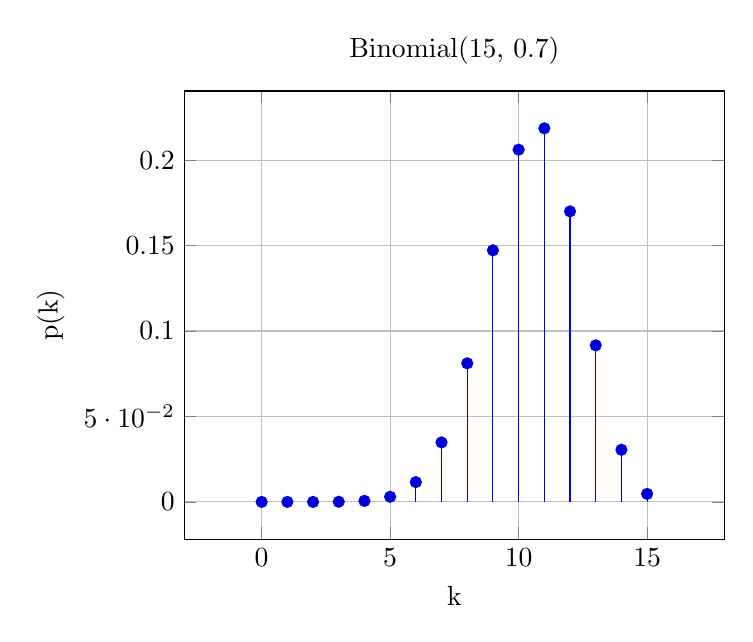
\begin{tikzpicture}
		\begin{axis}[enlarge x limits=0.2, grid = both,
			xlabel = k, ylabel = p(k), title = {Binomial(15, 0.7)}]
			\addplot+[ycomb] plot coordinates {( 0 , 0.0 ) ( 1 , 0.0 ) ( 2 , 0.0 ) ( 3 , 0.0001 ) ( 4 , 0.0006 ) ( 5 , 0.003 ) ( 6 , 0.0116 ) ( 7 , 0.0348 ) ( 8 , 0.0811 ) ( 9 , 0.1472 ) ( 10 , 0.2061 ) ( 11 , 0.2186 ) ( 12 , 0.17 ) ( 13 , 0.0916 ) ( 14 , 0.0305 ) ( 15 , 0.0047 ) };  
		\end{axis} 
	\end{tikzpicture}
\end{figure}


The two defining parameters of a Binomial RV are $ (n, p) $ where $ n $ is the number of trials and $ p $, the probability of each trial being independently a success.

\begin{align}
	P \left\{X = i\right\} &= \binom{n}{i}\ p^i \ (1-p)^{n-i}
\end{align}

Proving the normalization constraint requires the binomial theorem,
\begin{align}
	[p + (1-p)]^n &= 1^n = 1 \nonumber \\
	%
	\sum\limits_{i=0}^{n} P \left\{X = i\right\} &= \sum\limits_{i=0}^{n} \binom{n}{i}\ p^i \ (1-p)^{n-i}  = 1
\end{align}

Using the fact that the $ \mathbb{E}[\sum X] $ when the RVs are independent, reduces to $ \sum \mathbb{E}[X] $, and a similar rule for the variance,

\begin{align}
	\mathbb{E}[X] &= np \\
	%
	\mathrm{Var}(X) &= np(1-p)
\end{align}

If $ X_1, X_2 $ are two binomial RVs with parameters $ (n_1, p) $ and $ (n_2, p) $, then the RV $ X = X_1 + X_2 $ is also a binomial RV with parameters $ (n_1 + n_2, p) $ 

\textbf{Poisson RV} : Consider an RV that takes on non-negative integer values along with a parameter $ \lambda > 0 $, whose PMF is given by


\begin{align}
	P \left\{X = i\right\} &= e^{-\lambda}\ \frac{\lambda^i}{i!}
\end{align}

Using the Taylor series expansion of the exponential function, the normalization constraint is proved as follows,


\begin{align}
	e^x &= 0 + 1 + \frac{x^2}{2!} + \frac{x^3}{3!} + \dots \nonumber \\
	%
	\sum\limits_{i=0}^{\infty} P \left\{X = i\right\} &= e^{-\lambda} \left(\sum\limits_{i=0}^{\infty} \frac{\lambda^i}{i!}\right) = e^{-\lambda} \ e^{\lambda} = 1
\end{align}

\begin{figure}[!h]
	\centering
	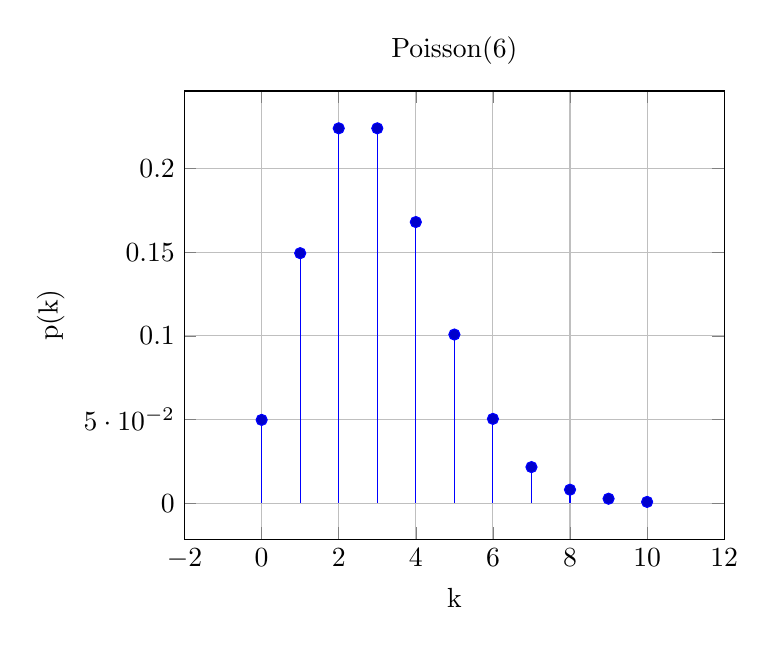
\begin{tikzpicture}
		\begin{axis}[enlarge x limits=0.2, grid = both,
			xlabel = k, ylabel = p(k), title = {Poisson(6)}]
			\addplot+[ycomb] plot coordinates {( 0 , 0.0498 ) ( 1 , 0.1494 ) ( 2 , 0.224 ) ( 3 , 0.224 ) ( 4 , 0.168 ) ( 5 , 0.1008 ) ( 6 , 0.0504 ) ( 7 , 0.0216 ) ( 8 , 0.0081 ) ( 9 , 0.0027 ) ( 10 , 0.0008 ) };  
		\end{axis} 
	\end{tikzpicture}
\end{figure}

Using the derivatives of the moment-generating function $ \phi(t) $, gives the mean and variance,

\begin{align}
	\phi(t) &= \mathbb{E}[e^{tX}] = \exp\left\{\lambda (e^t - 1)\right\}\\
	%
	\mathbb{E}[X] &= \lambda \\
	%
	\mathrm{Var}(X) &= \lambda
\end{align}

In the limit of $ n $ very large and $ p $ very small for a binomial RV with parameters $ (n, p) $, it can be approximated using a Poisson RV with parameter $ \lambda = np $.

\begin{align}
	P \left\{X = i\right\}\ =\ \binom{n}{i}\ p^i\ (1-p)^{n-i}\ \approxeq\ e^{-np}\ \frac{(np)^i}{i!}
\end{align}

An evern more general result, uses $ n $ independent trials each with probability of success $ p_i \ \forall\ i \in \left\{1, \dots, n\right\}$, with the condition that $ n $ is large and all of the $ p_i $ are small. The Poisson RV approximation can then me made with parameter $ \lambda = \sum p_i $.

Weak independence is measured by the conditional probability of one event succeeding given another has already succeeded. If these two values are approximately equal, then this approximation applies.

If $ X_1, X_2 $ are independently Poisson distributed with parameters $ \lambda_1, \lambda_2 $, then their sum $ X = X_1 + X_2 $ is also Poisson distributed with parameter $ \lambda_1 + \lambda_2 $. Since the moment generating function of a distribution uniquely determines it,

\begin{align}
	\phi (t) &= \mathbb{E}[e^{tX}] = \mathbb{E}[e^{t(X_1 + X_2)}] \nonumber \\
	%
	&= \mathbb{E}[e^{tX_1}] \mathbb{E}[e^{tX_2}] \nonumber \\
	%
	&= \exp\left\{(\lambda_1 + \lambda_2) (e^t - 1)\right\}
\end{align}

As an extension of the above, consider a total of $ N $ events, of which $ N_1, N_2 $ represent the number of events of types 1 and 2, with probabilities $ p $ and $ 1-p $ respectively. Also, $ N = N_1 + N_2 $.

If $ N $ is Poisson distributed with mean $\lambda$, then $ N_1, N_2 $ are also Poisson distributed with mean $ p\lambda $ and $ (1-p)\ \lambda $ respectively. This easily extends to more than two possible event types.

\begin{align}
	P\left\{N = n+m\right\} &= e^{-\lambda} \ \frac{\lambda^{n+m}}{(n+m)!} \nonumber \\
	%
	P\left\{N_1 = n\right\} &= e^{-p\lambda} \ \frac{(p\lambda)^{n}}{(n)!} \nonumber \\
	%
	P\left\{N_2 = m\right\} &= e^{-(1-p)\lambda} \ \frac{((1-p)\lambda)^{m}}{(m)!}
\end{align}

\textbf{Hypergeometric RV} : Consider a set of $ N+M $ objects of which $ N $ are acceptable and $ M $ defective. Let an experiment involve choosing $ n $ random objects out of $ N+M $, and then measure the number of acceptable objects picked using the RV $ X $.

$ X \in \left\{0, 1, \dots, \min(n, N) \right\} $, as the number of acceptable objects picked cannot exceed $ N $. This is a hypergeometric RV with PMF given by,

\begin{align}
	P \left\{X = i\right\} &= \ddfrac{\binom{N}{i}\ \binom{M}{n-i}}{\binom{N+M}{n}}
\end{align}

The parameters are $ (N, M, n) $, with the RV taking on non-negative integer values. If the proportion of acceptable objects is $ p $, then,

\begin{align}
	\mathbb{E}[X] &= \frac{nN}{N+M} = np \\
	%
	\mathrm{Var}(X) &= \frac{nNM}{(N+M)^2}\ \left(1 - \frac{n-1}{N+M-1}\right) \nonumber \\
	%
	&=  np\ (1-p)\ \left(1 - \frac{n-1}{N+M-1}\right)
\end{align}

Notice from the variance that the hypergeometric distribution converges to a binomial distribution in the limit $ N+M \to \infty $ and thus $ n \lll N $.

Consider two binomial RVs $ X, Y $ with parameters $ (n, p) $ and $ (m, p) $ respectively. The PMF of $ X $, given $ X+Y = k $ is given by,

\begin{align}
	P \left\{X = i\ |\ X+Y = k\right\} &= \ddfrac{\binom{n}{i}\ \binom{m}{k-i}}{\binom{n+m}{k}}
\end{align}

The denominator uses the fact that $ X+Y $ is also binomial with paramters $ (n+m, p) $, and the expression measures the probability that $ i $ out of the $ k $ successes were contributed by the RV $ X $.

This turns out to be a hypergeomtric RV measuring how many out of $ k $ objects picked were of type $ X $.


\textbf{Uniform RV} : Consider a continuous RV over the closed interval $ \left[\alpha, \beta\right] $, with PDF given by

\begin{align}
	f(x) &= \frac{1}{\beta - \alpha} & \text{if}\ x \in \left[\alpha, \beta\right] \\
	%
	f(x) &= 0 & \text{otherwise} \nonumber
\end{align}

The normalization constriant is easily proven using the Riemann integration of a continuous function.

\begin{align}
	P \left\{a < X < b\right\} &= \int\limits_{a}^{b} f(x)\ \mathrm{d} x = \frac{b - a}{\beta - \alpha} \\
	%
	P \left\{-\infty < X < \infty\right\} &= \int\limits_{-\infty}^{\infty} f(x)\ \mathrm{d} x = 1 \nonumber
\end{align}

Using simple polynomial integrations,

\begin{align}
	\mathbb{E}[X] &= \frac{\alpha + \beta}{2} \\
	%
	\mathrm{Var}(X) &= \frac{(\beta - \alpha)^2}{12} 
\end{align}


By computer science convention, a \textit{random number} is a uniformly distributed real number in the range $ [0, 1] $. A simple linear transformation $ Y = aX + b $ can be used to rescale this random number to the domain $ [b, a+b] $.

An important application of uniform RV sampling is Monte Carlo simulations, often used to estimate a parameter by performing a large number of experiments and using a frequentist approach to assign probabilities.

\textbf{Normal RV} : The most consistent distribution underlying real-world datasets, and as a result the most well-studied. This was originally introduced as an approximation to binomial distributions with extremely large $ n $. Using the mean and variance as parameters, the PDF for $ X \sim \mathcal{N}(\mu, \sigma^2) $ is defined as

\begin{align}
	f(x) = \frac{1}{\sqrt{2 \pi \sigma^2}} \exp \left[\frac{- (x - \mu)^2}{2\sigma^2}\right] \qquad \forall \quad x \in \mathbb{R}
\end{align}

This distribution is also called a bell curve. It is symmetric about $ \mu $, which is also its maximum.

\begin{align}
	\mathbb{E}[X] &= \mu \\
	%
	\mathrm{Var}(X) &= \sigma^2 \\
	%
	\mathbb{E}[aX + b] &= a\ \mu + b \nonumber \\
	%
	\mathrm{Var}(aX + b) &= a^2 \ \sigma^2 \nonumber 
\end{align}

\textit{Standard normal RV} : A normal RV with mean 0 and variance 1. Any normal RV $ X $ can be converted into a standard normal RV ($ \Phi $), using the transform $ Z = (X - \mu) / \sigma$

\begin{align}
	X &\sim \mathcal{N}(\mu, \sigma^2) \nonumber \\
	%
	Z &\sim \mathcal{N}(0, 1) \qquad \text{using} \qquad Z = \frac{X - \mu}{\sigma}
\end{align}

\begin{figure}[H]
	\centering
	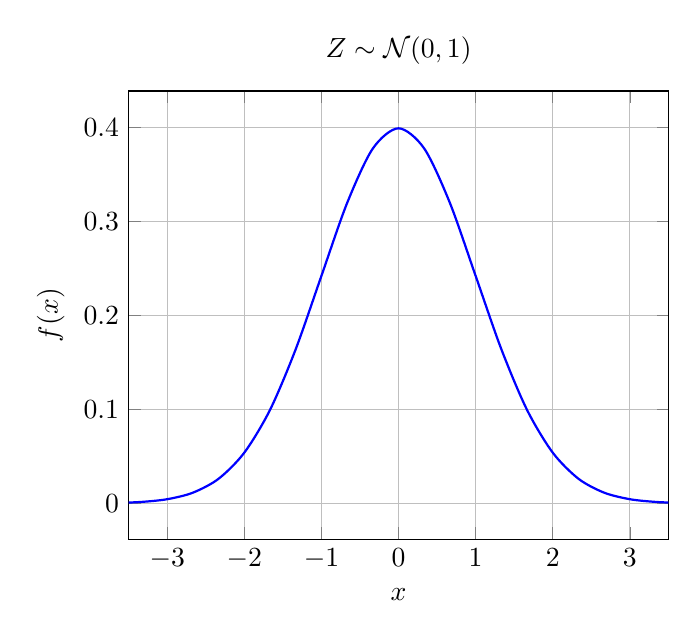
\begin{tikzpicture}
		\begin{axis}[xlabel=$x$, grid = both, xmin = -3.5, xmax = 3.5, ylabel = {$f(x)$}, title = {$ Z \sim \mathcal{N}(0, 1) $}]
			\addplot[thick, smooth, draw=blue][name path = f2, domain = -4:4]{(1/sqrt(2*pi)*exp(-x*x*0.5))};
		\end{axis}
	\end{tikzpicture}
\end{figure}

The numerical value of the standard normal RV $ (\Phi) $ has historically been computed using approximations and the CDF tabulated to a high degree of precision. Such a reference table is used to actually assign probabilities to $ \Phi $ 

\begin{align}
	\Phi(x) &= \int\limits_{-\infty}^{x} \frac{1}{\sqrt{2 \pi}} \exp \left(\frac{-y^2}{2}\right)\ \mathrm{d}y \\
	%
	P\left\{X < b\right\} &= P \left\{\frac{X - \mu}{\sigma} < \frac{b - \mu}{\sigma}\right\} = \Phi \left\{\frac{b - \mu}{\sigma}\right\} \\
	%
	\Phi(-x) &= 1 - \Phi(x)
\end{align}

The moment generating function of a normal RV uses the result for a standard normal RV.

\begin{align}
	\phi_Z (t) &= \mathbb{E}[e^{tZ}] = \exp\left(\frac{t^2}{2}\right)	  \\
	%
	\phi_X (t) &= \mathbb{E}[e^{t\mu}\ e^{t \sigma Z}] = \exp\left(\mu t + \frac{\sigma^2 t^2}{2}\right)
\end{align}

This also leads to the fact that the sum of independent normal RVs is also a normal RV. Consider a set of normal RVs $ \left\{X_i\right\} $ with mean and variance $ \left\{\mu_i\right\},\ \left\{\sigma^2_i\right\} $ respectively. From the moment-generating function,

\begin{align}
	\mathbb{E}[e^{tX}] &= \prod_{i=1}^{n} \mathbb{E}[e^{tX_i}] \nonumber \\
	%
	\mu &= \sum\limits_{i=1}^{n} \mu_i \qquad \text{and} \qquad \sigma^2 = \sum\limits_{i=1}^{n} \sigma_i^2
\end{align}

\textit{Percentile and z-score} : By convention, $ \alpha $ and $ z_\alpha $ are called the \textit{p-value} and \textit{z-score} respectively. The $ 100 \alpha $ percentile of a standard normal RV is that value $ x = z_\alpha $ for which,

\begin{align}
	P \left\{Z > z_\alpha\right\} &= 1 - \Phi(z_\alpha) = \alpha
\end{align}

\begin{figure}[H]
	\centering
	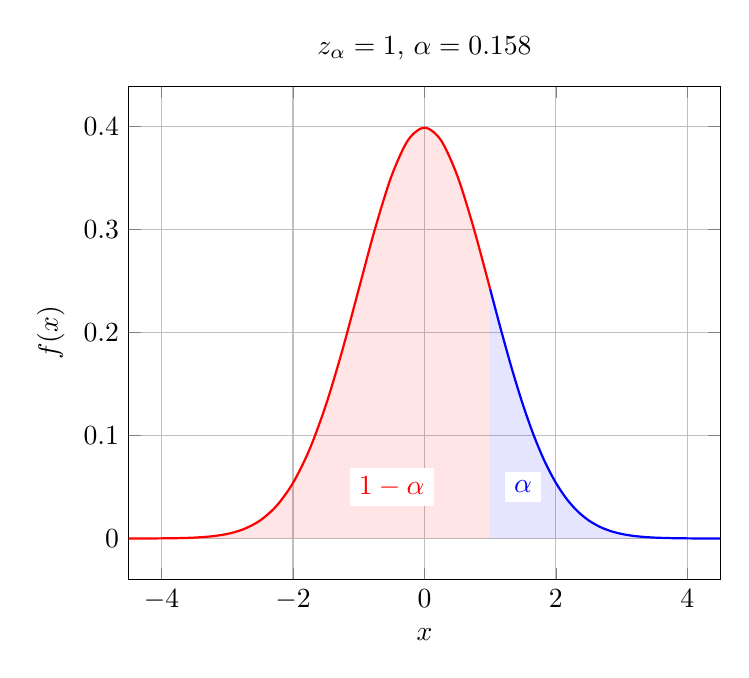
\begin{tikzpicture}
		\begin{axis}[width = 0.75\textwidth,xlabel=$x$, ylabel=$ f(x) $, grid = both, xmin = -4.5, xmax = 4.5, title = {$z_\alpha = 1$, $ \alpha = 0.158 $}]
			\addplot[thick, smooth, draw=red][name path = f1, domain = -5:1]{(1/sqrt(2*pi)*exp(-x*x*0.5))};
			\addplot[thick, smooth, draw=blue][name path = f2, domain = 1:5]{(1/sqrt(2*pi)*exp(-x*x*0.5))};
			
			\path[name path=axis1] (axis cs:-5,0) -- (axis cs:1,0);
			\path[name path=axis2] (axis cs:1,0) -- (axis cs:5,0);
			
			\addplot [thick,color=red,fill=red, fill opacity=0.1] fill between[of=f1 and axis1,];
			\addplot [thick,color=red,fill=blue, fill opacity=0.1] fill between[of=f2 and axis2,];
			
			\node[color=blue, fill=white] at (axis cs: 1.5,.05) {$ \alpha $};
			\node[color=red, fill=white] at (axis cs: -0.5,.05) {$ 1 - \alpha $};
			
		\end{axis}
	\end{tikzpicture}
\end{figure}


\textbf{Exponential RV} :  Consider a continuous RV defined over the real line with PDF and CDF given by

\begin{align}
	f(x) &= \lambda\ e^{-\lambda x} & \text{if}\ x \in \left[0, \infty\right) \\
	%
	f(x) &= 0 & \text{otherwise} \nonumber
\end{align}


\begin{figure}[H]
	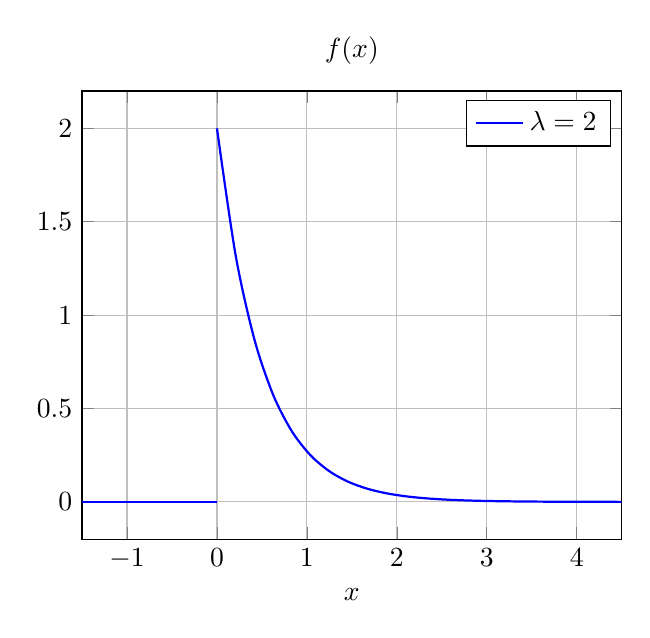
\begin{tikzpicture}
		\begin{axis}[xlabel=$x$, grid = both, xmin = -1.5, xmax = 4.5, title = {$f(x)$}]
			\addplot[thick, smooth, draw=blue][name path = f1, domain = -2:0]{0};
			\addplot[thick, smooth, draw=blue][name path = f1, domain = 0:5]{2*exp(-2*x)};
			\addlegendentry{$ \lambda = 2$}
		\end{axis}
	\end{tikzpicture}
	%
	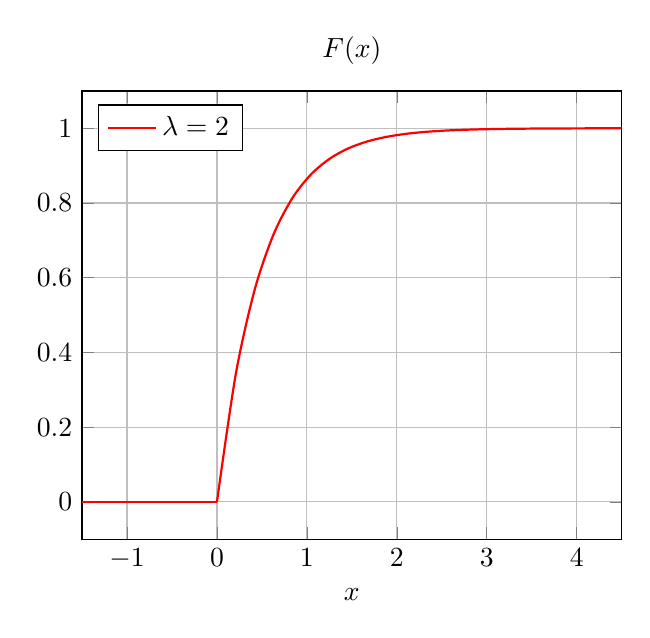
\begin{tikzpicture}
		\begin{axis}[xlabel=$x$, grid = both, xmin = -1.5, xmax = 4.5, title = {$F(x)$}, legend pos = north west]
			\addplot[thick, smooth, draw=red][name path = f1, domain = -2:0]{0};
			\addplot[thick, smooth, draw=red][name path = f1, domain = 0:5]{1 - exp(-2*x)};
			\addlegendentry{$ \lambda = 2$}
		\end{axis}
	\end{tikzpicture}
\end{figure}


The parameter $ \lambda $ , called the \textit{rate}, solely defines the exponential RV with a CDF,

\begin{align}
	F(x) &= 1 - e^{-\lambda x} \qquad \forall \ x \geq 0
\end{align}

The exponential distribution if observed most commonly as the distribution of time intervals between successive occurrences of natural events. The moment-generating function gives the mean and variance as follows

\begin{align}
	\phi(t) &= \frac{\lambda}{\lambda - t} \qquad \forall\ t < \lambda \\
	%
	\mathbb{E}[X] &= \frac{1}{\lambda} \\
	%
	\mathrm{Var}(X) &= \frac{1}{\lambda^2}
\end{align}

An important property exclusive to the exponential function is that it is \textit{memoryless}, or \textit{self-similar} across time. This is mathematically represented as

\begin{align}
	P \left\{X > t+s\ |\ X > t \right\} &= P \left\{X > s \right\} \qquad \forall \ s, t\geq 0
\end{align}

The probability of an item functioning for $ s $ additional time does not depend on the fact that it has functioned for $ t $ time already.

The minimum of a set of independent exponential RVs $ \left\{X_i\right\} $ with parameters $ \left\{\lambda_i\right\} $ is also an exponential RV. This is easily understood as the lifetime of a system with many components all of which are necessary for it to function.

\begin{align}
	P \left\{\mathrm{min}(X_1, X_2, \dots, X_n) > x\right\} &= e^{-\lambda x} \nonumber \\
	%
	\lambda &= \sum_{i=1}^{n} \lambda_i
\end{align}

An independent exponential RV transforming as $ X \to cX $ causes the rate to change as $ \lambda \to \lambda/c $.

\textbf{Poisson process} : Consider a process where events happen randomly such that $ N(t) $ denotes the number of events in the time $ [0, t] $. This is a Poisson process with \textit{rate} $ \lambda $, if

\begin{itemize}
	\item $ N(0) = 0 $, with $ t = 0 $ denoting the start of the process.
	
	\item Disjoint time intervals have an independent number of events occurring in them.
	
	\item The number of events in a given interval has a distribution depending only on the length of the interval.
	
	\item In the limit of a small time interval of length $ h \to 0 $, the probability of event occurrence
	
	\begin{align}
		P \left\{N(h) = 1\right\} &\approx \lambda h \nonumber \\
		%
		P \left\{N(h) \geq 2\right\} &\approx 0
	\end{align}
\end{itemize}

The distribution of the number of events occurring in any interval of length $ t $ in a Poisson process is a Poisson RV with parameter $ \lambda t $.

\begin{align}
	P \left\{N(t) = k\right\} &= e^{-\lambda t} \ \frac{(\lambda t)^k}{k!}
\end{align}

For a Poisson process, let $ Y_n $ denote the time interval between the $ (n-1)^{th} $ and $ n^{th} $ events for all $ n > 1 $. This set $ \left\{Y_n\right\} $ is called \textit{inter-arrival time}. Then, the set $ Y_n $ are all independent RVs having an exponential distribution with parameter $ \lambda $ 

\textbf{Pareto RV} : Using the self-similarity of the exponential RV, the Pareto distribution is used to exmaine the distribution of income among a population and to identify what proportion of the total income earned by a population is contributed by the top earners.

Consider an exponential RV $ X $ with rate $ \lambda $. The Pareto RV with minimum parameter $ \alpha $ and index parameter $ \lambda > 0$, is given by

\begin{align}
	Y &= \alpha\ e^{X} \\
	%
	X &= \lambda\ e^{-\lambda x} & \text{if}\ x \in \left[0, \infty\right) \nonumber
\end{align}

This RV is constrained by $ Y \geq \alpha $. The CDF of the Pareto distribution is

\begin{align}
	P \left\{Y > y\right\} &= \left(\frac{\alpha}{y}\right)^\lambda \nonumber \\
	%
	F_Y(y) &= 1 - \left(\frac{\alpha}{y}\right)^\lambda \qquad \forall \  y \geq \alpha \\
	%
	f_Y(y) &= \frac{\lambda}{y}\ \left(\frac{\alpha}{y}\right)^\lambda \qquad \forall \  y \geq \alpha
\end{align}

\begin{figure}[H]
	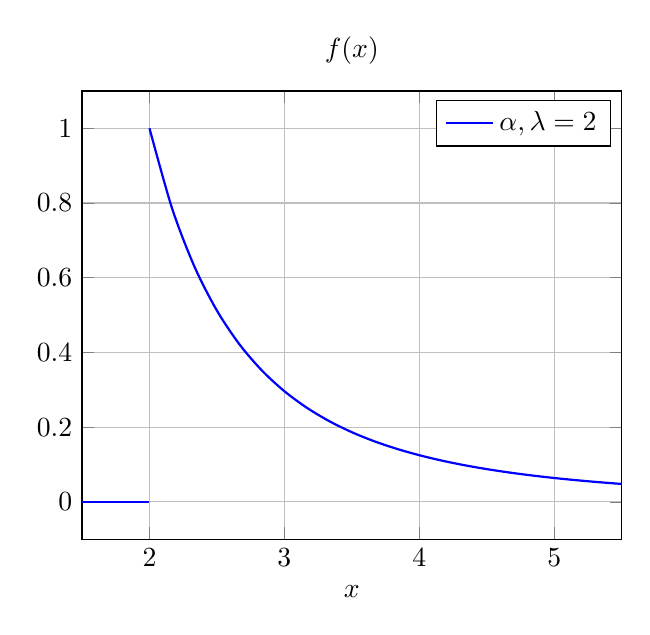
\begin{tikzpicture}
		\begin{axis}[xlabel=$x$, grid = both, xmin = 1.5, xmax = 5.5, title = {$f(x)$}]
			\addplot[thick, smooth, draw=blue][name path = f1, domain = 0:2]{0};
			\addplot[thick, smooth, draw=blue][name path = f1, domain = 2:6]{8/(x^(3))};
			\addlegendentry{$ \alpha, \lambda = 2$}
		\end{axis}
	\end{tikzpicture}
	%
	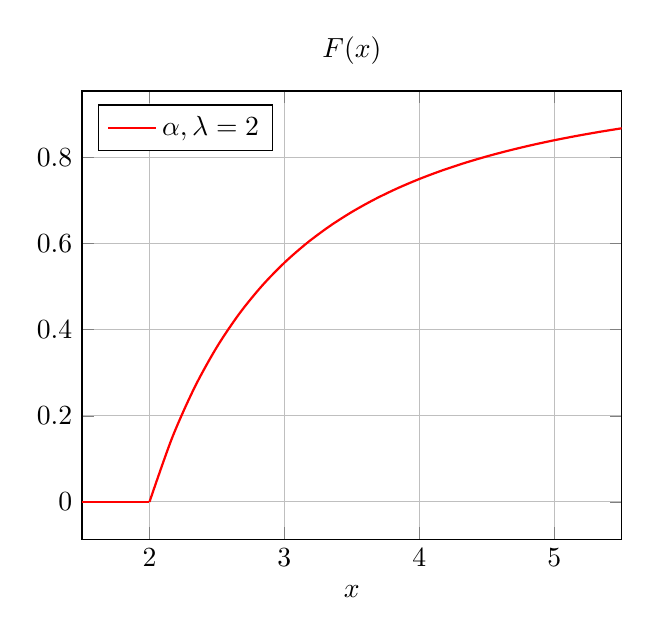
\begin{tikzpicture}
		\begin{axis}[xlabel=$x$, grid = both, xmin = 1.5, xmax = 5.5, title = {$F(x)$}, legend pos = north west]
			\addplot[thick, smooth, draw=red][name path = f1, domain = 0:2]{0};
			\addplot[thick, smooth, draw=red][name path = f1, domain = 2:6]{1 - (2/x)^2};
			\addlegendentry{$ \alpha, \lambda = 2$}
		\end{axis}
	\end{tikzpicture}
\end{figure}

The expected value is finite only for $ \lambda > 1 $,

\begin{align}
	\mathbb{E}(Y) &= \alpha \ \frac{\lambda}{\lambda - 1 }
\end{align}

As a result of the self-similarity of the exponential distribution, the Pareto RV is also self-similar. Given the condition $ Y > y_0 $ for some $ y_0 > \alpha $, this conditional distribution is also Pareto with parameters $ y_0 $ and $ \lambda $.

\begin{align}
	P \left\{Y > y\ |\ Y > y_0 \right\} = \left(\frac{y_0}{y}\right)^\lambda
\end{align}

\textbf{Gamma distribution} : Consider the gamma function $ \Gamma(x) $ defined by an integral which can be recursively related to itself.

\begin{align}
	\Gamma(\alpha) &= \int\limits_{0}^{\infty} e^{-y}\ y^{\alpha -1}\ \mathrm{d}y \\
	%
	\Gamma(\alpha) &= (\alpha - 1)\ \Gamma(\alpha - 1)
\end{align}

For the special case of integer values of $ \alpha $, and using $ \Gamma(1) = 1 $,
\begin{align}
	\Gamma(n) &= (n - 1)\ \Gamma(n - 1) \nonumber \\
	%
	\Gamma(n) &= (n-1)!	
\end{align}

The Gamma RV with parameters $ \alpha, \lambda > 0 $, is now defined using the PDF,

\begin{align}
	f(x) &= \lambda\ e^{- \lambda x}\ \frac{(\lambda x)^{\alpha-1}}{\Gamma(\alpha)} \qquad \forall\ x \geq 0 \\
	%
	&= 0 \qquad \text{otherwise} \nonumber
\end{align}

\begin{figure}[H]
	\centering
	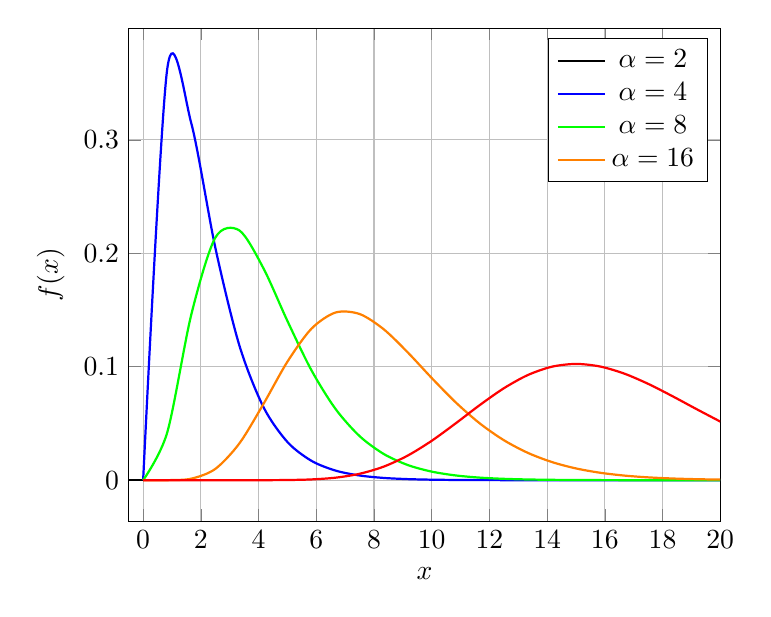
\begin{tikzpicture}
		\begin{axis}[width = 0.75\textwidth,xlabel=$x$, ylabel=$ f(x) $, grid = both, xmin = -0.5, xmax = 20]
			\addplot[thick, smooth, draw=black][name path = f1, domain = -1:0]{0};
			\addplot[thick, smooth, draw=blue][name path = f2, domain = 0:20]{e^(-x)*x};
			\addplot[thick, smooth, draw=green][name path = f3, domain = 0:20]{e^(-x)*(x^3)/6};
			\addplot[thick, smooth, draw=orange][name path = f4, domain = 0:20]{e^(-x)*(x^7)/5040};
			\addplot[thick, smooth, draw=red][name path = f5, domain = 0:20]{e^(-x)*(x^15)/1307674368000};
			\legend{$ \alpha = 2 $, $ \alpha = 4 $, $ \alpha = 8 $, $ \alpha = 16 $}
		\end{axis}
	\end{tikzpicture}
\end{figure}



The moment-generating function gives the mean and variance using

\begin{align}
	\phi(t) &= \left(\frac{\lambda}{\lambda - t}\right)^{\alpha} \\
	%
	\mathbb{E}[X] &= \frac{\alpha}{\lambda} \\
	%
	\mathrm{Var}(X) &= \frac{\alpha}{\lambda^2}
\end{align}

Using the moment-generating function above, the sum of many independent Gamma RVs $ \left\{X_i\right\} $ with parameters $ \left\{\alpha_i\right\} $ and a shared $ \lambda $, then their sum $ X = \sum X_i $ is also a Gamma RV with parameters $ \sum \alpha_i $ and $\lambda$.

This result further simplifies when $ \alpha = 1 $, making the Gamma RVs reduce to exponential RVs with the same rate parameter $ \lambda $. The sum of $ n $ independent exponential RVs $ \left\{X_i\right\} $ with a shared rate $ \lambda $, is a Gamma RV with parameters $ (n, \lambda) $.

Note the effect of multiplying a Gamma RV by a scalar. Let $ X $ be a Gamma RV which is multiplied by scalar $ b $, Now the moment-generating function of the new RV $ bX $ is

\begin{align}
	\mathbb{E}[e^{tX}] &= \left(\frac{\lambda}{\lambda - t}\right)^\alpha \nonumber \\
	%
	\mathbb{E}[e^{t\ bX}] &= \mathbb{E}[e^{bt\ X}] = \left(\frac{\lambda}{\lambda - bt}\right)^\alpha = \left(\frac{\lambda / b}{\lambda / b - t}\right)^\alpha \nonumber \\
	%
	bX &\sim \Gamma(\alpha, \lambda / b)  \qquad \text{if} \qquad X \sim \Gamma(\alpha, \lambda)
\end{align}

\textbf{Chi-square distribution} : Consider a set of independent standard normal RVs $ \left\{Z_i\right\} $. Then the RV defined as $ X \sim \chi_n^2 $ is given by

\begin{align}
	X = Z_1^2 + Z_2^2 + \dots + Z_n^2
\end{align}

$ X $ is a chi-squared RV with $ n $ \textit{degrees of freedom}. Similar to the p-value from the normal RV, $ \chi_{\alpha, n}^2 $ is defined as follows and tabulated using approximate computations.

\begin{align}
	P \left\{X \geq \chi_{\alpha, n}^2 \right\} = \alpha
\end{align}

The equivalence of the chi-squared and Gamma distributions can be seen through the moment-generating functions 

\begin{align}
	\phi(t) &= (1-2t)^{-n/2} \\
	%
	\phi(t) &= \left(\frac{1/2}{1/2 - t}\right)^{n/2} \nonumber
\end{align}

Thus, a chi-squared RV with $ n $ degrees of freedom is the same as a Gamma distribution with parameters $ (n/2, 1/2) $.

\begin{align}
	\mathbb{E}[X] &= \frac{n/2}{1/2} = n \\
	%
	\mathrm{Var}(X) &= \frac{n/2}{(1/2)^2} = 2n
\end{align}

\textbf{t-distribution} : Using a standard normal RV $ Z $ and a chi-square RV $ \chi_n^2 $ with $ n $ degrees of freedom, the t-distribution is defined as,

\begin{align}
	T_n = \frac{Z}{\sqrt{\chi_n^2 / n}}
\end{align}

The t-distribution is also symmetric about $ x=0 $ like $ Z $, but with longer tails. It increasingly resembles $ Z $ as $ n \to \infty $. To prove this, use the weak law of large numbers on the denominator above.

\begin{align}
	\mathbb{E}[X] &= 0 \qquad n>1 \\
	%
	\mathrm{Var}(X) &= \frac{n}{n-2} \qquad n>2
\end{align}

Similar to the p-value from the normal RV, $ t_{\alpha, n} $ is defined as follows and tabulated using approximate computations.

\begin{align}
	P \left\{T_n \geq t_{\alpha, n} \right\} &= \alpha \\
	%
	t_{1-\alpha, n} &= -t_{\alpha, n} \nonumber
\end{align}

\textbf{F-distribution} : Let $ \chi_n^2, \chi_m^2 $ be chi-square RVs with $ n, m $ degrees of freedom respectively. Then,

\begin{align}
	F_{n,m} = \frac{\chi_n^2 / n}{\chi_m^2 / m}
\end{align}

is an F-distribution with$ n,m $ degrees of freedom.

Similar to the p-value from the normal RV, $ F_{\alpha, n, m} $ is defined as follows and tabulated using approximate computations.

\begin{align}
	P \left\{F_{n,m} \geq F_{\alpha, n, m} \right\} &= \alpha \\
\end{align}

\newpage


%\include{./TeX_files/exercise05}
%\chapter{Distributions of Sampling Statistics}


\begin{flushright}
	\textit{``Just find a way to jam it into the Central Limit Theorem"}
\end{flushright}

Most real world populations are intractably large and the statistics of the entire population are impossible to arrive at using brute-force computation. The use of a well-drawn sample to estimate the statistics of the underlying population is the most-used workaround to this problem.

\textbf{Random sample} : A set of random variables which are independent and have a common distribution $ F $. When $ F $ is only specified up to some parameters that are not known, it is possible to estimate these parameters using the statistics of the random sample.

Depending on whether any information about the form of $ F $ is known, this is called either a  \textit{parametric} inference problem, or a \textit{non-parametric} inference problem. An example of the latter is knowing only whether $ F $ is continuous or discrete and nothing further.

\textbf{Statistic} : A RV which is determined by the random sample instead of the underlying population. The two most interesting statistics are the sample mean and the sample variance.

\textbf{Sample mean} : Consider a population with mean $ \mu $ and variance $ \sigma $, without any information about the specific probability distribution. In contrast to the population mean and variance, the \textit{sample mean} of a random sample $ \left\{X_i\right\} $ is defined as

\begin{align}
	\overline{X} &= \frac{X_1 + X_2 + \dots + X_n}{n}
\end{align}

$ \overline{X} $ is also an RV, whose expected value and variance are

\begin{align}
	\mathbb{E}[\overline{X}] &= \frac{1}{n}\ \left(\mathbb{E}[X_1] + \dots + \mathbb{E}[X_n]\right) = \mu \\
	%
	\mathrm{Var}(\overline{X}) &= \frac{1}{n^2}\ \left[\mathrm{Var}(X_1) + \dots + \mathrm{Var}(X_n)\right] = \frac{\sigma^2}{n}
\end{align}

The sample mean from an underlying standard normal population for different values of sample size, is itself a normal RV with spread decreasing as $ n $ increases.

\begin{figure}[H]
	\centering
	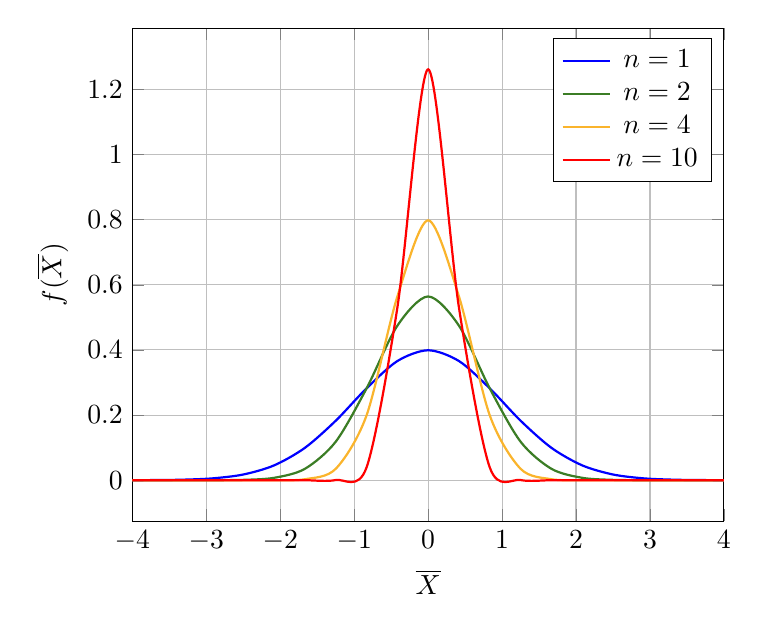
\begin{tikzpicture}
		\begin{axis}[width = 0.75\textwidth,xlabel=$\overline{X}$, ylabel=$ f(\overline{X}) $, grid = both, xmin = -4, xmax = 4]
			\addplot[thick, smooth, draw=blue][name path = f2, domain = -5:5]{(1/sqrt(2*pi))*e^(-0.5*x*x)};
			\addplot[thick, smooth, draw=OliveGreen][name path = f3, domain = -5:5]{(1/sqrt(pi))*e^(-0.5*2*x*x)};
			\addplot[thick, smooth, draw=Dandelion][name path = f4, domain = -5:5]{(1/sqrt(0.5*pi))*e^(-0.5*4*x*x)};
			\addplot[thick, smooth, draw=red][name path = f5, domain = -5:5]{(1/sqrt(0.2*pi))*e^(-0.5*10*x*x)};
			\legend{$n=1$,$n=2$,$n=4$, $n=10$}
		\end{axis}
	\end{tikzpicture}
\end{figure}

\textbf{Central Limit Theorem} : Let $ \left\{X_i\right\} $ be independent identically distributed RV having the same mean $ \mu $ and variance $ \sigma^2 $.

In the limit of large $ n $, the distribution of $ \sum X_i $ is approximately normal with mean $ n\mu $ and variance $ n\sigma^2 $, regardless of the probability distribution of the individual $ X_i $ 

\begin{align}
	\frac{X_1 + X_2 + \dots + X_n - n\mu}{\sqrt{n}\ \sigma} &\sim Z
\end{align}

Consider the specific case of a binomial RV with parameters $ (n, p) $. This is decomposed into a set of $ n $ binary indicator RVs. Then for large $ n $,

\begin{align}
	X &= X_1 + X_2 + \dots + X_n \nonumber \\
	%
	\mathbb{E}[X_i] &= p \nonumber \\
	%
	\mathrm{Var}(X_i) &= (1-p) \nonumber \\
	%
	\frac{X - np}{\sqrt{np(1-p)}} & \sim Z 
\end{align}

\begin{figure}[!h]
	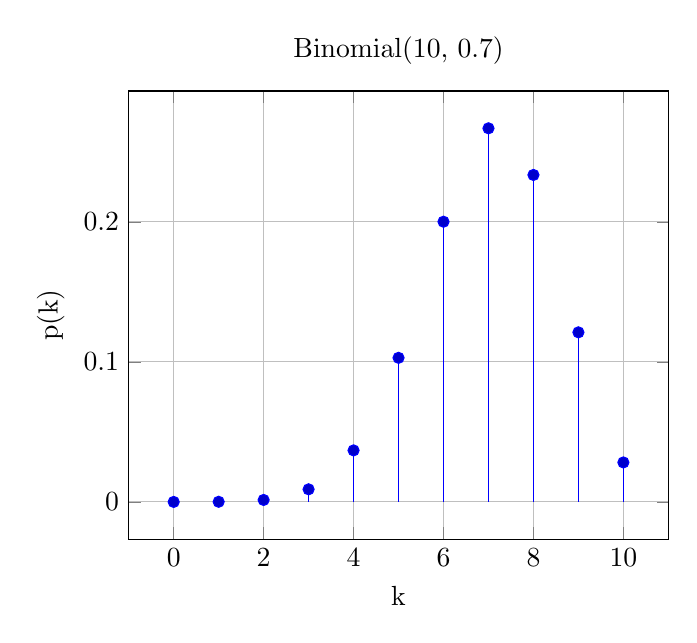
\begin{tikzpicture}
		\begin{axis}[grid = both,
			xlabel = k, ylabel = p(k), title = {Binomial(10, 0.7)}]
			\addplot+[ycomb] plot coordinates {( 0 , 0.0 ) ( 1 , 0.0001 ) ( 2 , 0.0014 ) ( 3 , 0.009 ) ( 4 , 0.0368 ) ( 5 , 0.1029 ) ( 6 , 0.2001 ) ( 7 , 0.2668 ) ( 8 , 0.2335 ) ( 9 , 0.1211 ) ( 10 , 0.0282 ) 
			 };  
		\end{axis} 
	\end{tikzpicture}
	%
	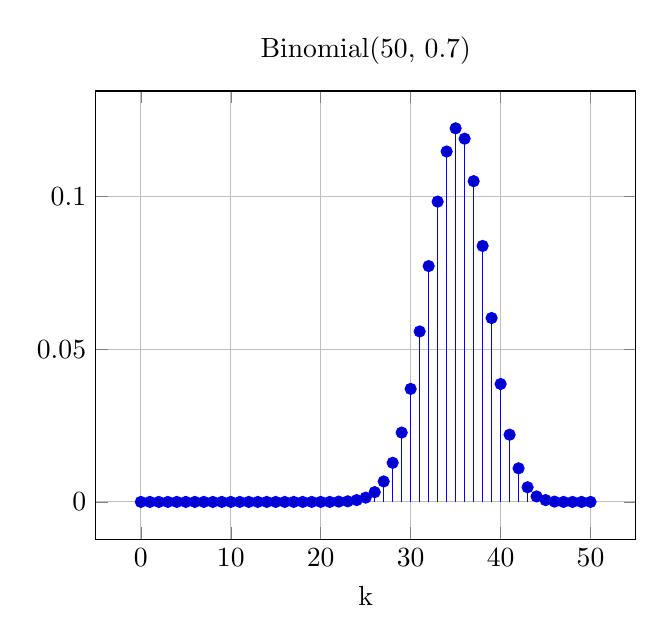
\begin{tikzpicture}
		\begin{axis}[grid = both, yticklabel style={
				/pgf/number format/fixed,
				/pgf/number format/precision=2
			},
			xlabel = k, title = {Binomial(50, 0.7)}]
			\addplot+[ycomb] plot coordinates {( 0 , 0.0 ) ( 1 , 0.0 ) ( 2 , 0.0 ) ( 3 , 0.0 ) ( 4 , 0.0 ) ( 5 , 0.0 ) ( 6 , 0.0 ) ( 7 , 0.0 ) ( 8 , 0.0 ) ( 9 , 0.0 ) ( 10 , 0.0 ) ( 11 , 0.0 ) ( 12 , 0.0 ) ( 13 , 0.0 ) ( 14 , 0.0 ) ( 15 , 0.0 ) ( 16 , 0.0 ) ( 17 , 0.0 ) ( 18 , 0.0 ) ( 19 , 0.0 ) ( 20 , 0.0 ) ( 21 , 0.0 ) ( 22 , 0.0001 ) ( 23 , 0.0002 ) ( 24 , 0.0006 ) ( 25 , 0.0014 ) ( 26 , 0.0032 ) ( 27 , 0.0067 ) ( 28 , 0.0128 ) ( 29 , 0.0227 ) ( 30 , 0.037 ) ( 31 , 0.0558 ) ( 32 , 0.0772 ) ( 33 , 0.0983 ) ( 34 , 0.1147 ) ( 35 , 0.1223 ) ( 36 , 0.1189 ) ( 37 , 0.105 ) ( 38 , 0.0838 ) ( 39 , 0.0602 ) ( 40 , 0.0386 ) ( 41 , 0.022 ) ( 42 , 0.011 ) ( 43 , 0.0048 ) ( 44 , 0.0018 ) ( 45 , 0.0006 ) ( 46 , 0.0001 ) ( 47 , 0.0 ) ( 48 , 0.0 ) ( 49 , 0.0 ) ( 50 , 0.0 ) 
			};  
		\end{axis} 
	\end{tikzpicture}
\end{figure} 

While the Poisson approximation to a Binomial RV is good for large $ n $ and small $ p $, this normal approximation is only good for large values of $ \sqrt{np(1-p)} $, with this value by convention being $ \geq 10 $.

The sample mean also obeys the central limit theorem for large values of sample size $ n $ to give,

\begin{align}
	\frac{\overline{X} - \mu}{\sigma / \sqrt{n}} &\sim Z
\end{align}

By convention, a sample size of at least $ 30 $ is needed to ensure that the sample mean will be approximately normal regardless of the underlying probability distribution. This minimum sample size is much smaller for specific distributions such as a normal RV ($ n \geq 1 $) and an exponential RV ($ n \geq 5 $)


\begin{figure}[H]
	\centering
	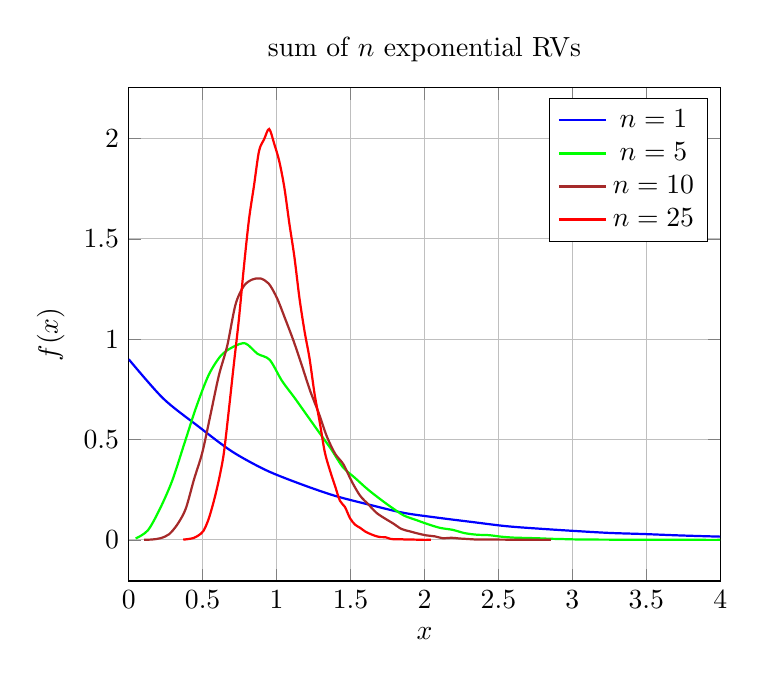
\begin{tikzpicture}
	\begin{axis}[width = 0.75\textwidth,grid = both, xmax = 4.0, xmin = 0,
		xlabel = $ x $, ylabel=$ f(x) $, title = sum of $ n $ exponential RVs]

		\addplot[smooth, thick, color = blue] plot coordinates {
			(0.0, 0.9003) (0.2322, 0.7054) (0.4643, 0.5692) (0.6965, 0.4414) (0.9286, 0.3473) (1.1607, 0.2788) (1.3929, 0.2199) (1.625, 0.1757) (1.8572, 0.1349) (2.0893, 0.1105) (2.3215, 0.0891) (2.5536, 0.0682) (2.7858, 0.0553) (3.0179, 0.0443) (3.2501, 0.0346) (3.4822, 0.0291) (3.7144, 0.0224) (3.9465, 0.0172) (4.1787, 0.013) (4.4108, 0.0109) (4.643, 0.0083) (4.8751, 0.0069) (5.1073, 0.0053) (5.3394, 0.0037) (5.5716, 0.0036) (5.8037, 0.0027) (6.0359, 0.0019) (6.268, 0.0015) (6.5002, 0.0012) (6.7323, 0.0009) (6.9645, 0.0009) (7.1966, 0.0006) (7.4288, 0.0006) (7.6609, 0.0002) (7.8931, 0.0002) (8.1252, 0.0002) (8.3574, 0.0002) (8.5895, 0.0003) (8.8217, 0.0001) (9.0538, 0.0002) (9.286, 0.0001) (9.5181, 0.0002) (9.7502, 0.0) (9.9824, 0.0) (10.2145, 0.0001) (10.4467, 0.0) (10.6788, 0.0) (10.911, 0.0) (11.1431, 0.0) (11.3753, 0.0001)
			
		}; 
		\addplot[smooth, thick, color = green] plot coordinates {
			(0.0473, 0.007) (0.1297, 0.0475) (0.2121, 0.1563) (0.2945, 0.2957) (0.3769, 0.4815) (0.4593, 0.6674) (0.5417, 0.823) (0.6241, 0.9185) (0.7064, 0.9618) (0.7888, 0.9792) (0.8712, 0.9273) (0.9536, 0.897) (1.036, 0.7929) (1.1184, 0.7112) (1.2008, 0.6257) (1.2832, 0.5401) (1.3656, 0.4557) (1.448, 0.3626) (1.5304, 0.3085) (1.6128, 0.254) (1.6952, 0.206) (1.7776, 0.1617) (1.86, 0.1217) (1.9424, 0.0994) (2.0248, 0.0776) (2.1071, 0.0595) (2.1895, 0.0501) (2.2719, 0.0336) (2.3543, 0.0257) (2.4367, 0.0234) (2.5191, 0.0159) (2.6015, 0.0113) (2.6839, 0.0096) (2.7663, 0.008) (2.8487, 0.0055) (2.9311, 0.004) (3.0135, 0.0024) (3.0959, 0.0022) (3.1783, 0.0013) (3.2607, 0.0011) (3.3431, 0.0007) (3.4255, 0.0007) (3.5078, 0.0006) (3.5902, 0.0001) (3.6726, 0.0006) (3.755, 0.0004) (3.8374, 0.0004) (3.9198, 0.0) (4.0022, 0.0001) (4.0846, 0.0002)
		}; 
		\addplot[smooth, thick, color = Brown] plot coordinates {
			(0.1048, 0.0005) (0.1609, 0.002) (0.2171, 0.0087) (0.2732, 0.0282) (0.3293, 0.0773) (0.3854, 0.1545) (0.4416, 0.3015) (0.4977, 0.4353) (0.5538, 0.6265) (0.6099, 0.82) (0.666, 0.9665) (0.7222, 1.1726) (0.7783, 1.2649) (0.8344, 1.2972) (0.8905, 1.3027) (0.9467, 1.2772) (1.0028, 1.2049) (1.0589, 1.1001) (1.115, 0.991) (1.1711, 0.8686) (1.2273, 0.742) (1.2834, 0.635) (1.3395, 0.516) (1.3956, 0.4294) (1.4518, 0.3765) (1.5079, 0.2915) (1.564, 0.2209) (1.6201, 0.1771) (1.6763, 0.1342) (1.7324, 0.1066) (1.7885, 0.0816) (1.8446, 0.0542) (1.9007, 0.0424) (1.9569, 0.0314) (2.013, 0.0223) (2.0691, 0.0176) (2.1252, 0.008) (2.1814, 0.0105) (2.2375, 0.0068) (2.2936, 0.0043) (2.3497, 0.0018) (2.4058, 0.0023) (2.462, 0.0018) (2.5181, 0.0012) (2.5742, 0.0011) (2.6303, 0.0009) (2.6865, 0.0002) (2.7426, 0.0002) (2.7987, 0.0) (2.8548, 0.0004)
		};
		\addplot[smooth, thick, color = red] plot coordinates {
			(0.3687, 0.0012) (0.4029, 0.0041) (0.4371, 0.0091) (0.4712, 0.0219) (0.5054, 0.0448) (0.5396, 0.1021) (0.5738, 0.1884) (0.6079, 0.2929) (0.6421, 0.4258) (0.6763, 0.6417) (0.7105, 0.8726) (0.7446, 1.0961) (0.7788, 1.3592) (0.813, 1.595) (0.8472, 1.7651) (0.8813, 1.938) (0.9155, 1.9959) (0.9497, 2.0477) (0.9839, 1.9737) (1.018, 1.8871) (1.0522, 1.7569) (1.0864, 1.5763) (1.1206, 1.4089) (1.1547, 1.2044) (1.1889, 1.04) (1.2231, 0.903) (1.2573, 0.7251) (1.2914, 0.5879) (1.3256, 0.4386) (1.3598, 0.3485) (1.394, 0.2718) (1.4281, 0.1955) (1.4623, 0.1639) (1.4965, 0.108) (1.5307, 0.0758) (1.5648, 0.06) (1.599, 0.0418) (1.6332, 0.0296) (1.6674, 0.0199) (1.7015, 0.0138) (1.7357, 0.0132) (1.7699, 0.005) (1.804, 0.0029) (1.8382, 0.0035) (1.8724, 0.0015) (1.9066, 0.0015) (1.9407, 0.0012) (1.9749, 0.0003) (2.0091, 0.0) (2.0433, 0.0006)
			
		};
	\legend{$n=1$,$n=5$,$n=10$, $n=25$}		
	\end{axis} 
	\end{tikzpicture}
\end{figure} 

\textbf{Sample variance} : Using the prior definition of the variance $ S^2 $, a sample drawn from an underlying distribution with parameters $ \mu, \sigma $ and sample mean $ \overline{X} $ has the sample variance $ S^2 $ defined as,

\begin{align}
	S^2 &= \ddfrac{\sum\limits_{i=1}^{n}(X_i - \overline{X})^2}{n-1}
\end{align}

The expected value of the sample variance is found using,

\begin{align}
	\sum\limits_{i=1}^{n}(x_i - \overline{x})^2 &= \sum\limits_{i=1}^{n}(x_i^2) - n\overline{x}^2 \nonumber \\
	%
	\mathbb{E}[X^2] &= \mathrm{Var}(X) + (\mathbb{E}[X])^2 \nonumber 
\end{align}

The derivation of $ \mathbb{E}[S^2] $, using the above relations is as follows,

\begin{align}
	(n-1)\mathbb{E}[S^2] &= \mathbb{E}\left[\sum\limits_{i=1}^{n}X_i^2\right] - n\mathbb{E}[\overline{X}^2] \nonumber \\
	%
	&= n\left[\mathrm{Var}(X_1) + (\mathbb{E}[X_1])^2 - \mathrm{Var}(\overline{X}) - (\mathbb{E}[\overline{X}])^2\right] \nonumber \\
	%
	&= n\sigma^2 + n\mu^2 - n(\sigma^2/n) - n\mu^2 \nonumber \\
	%
	\mathbb{E}[S^2] &= \sigma^2
\end{align}

\textbf{Sampling from a normal population} : For the specific case of samples drawn from an underlying population which is normally distributed $ X_i \sim \mathcal{N}(\mu, \sigma^2) $, the distribution of the sample mean and sample variance is of particular interest for real-world applications.

The sample mean $ \overline{X} $ is itself a normal RV, with mean $ \mu $ and variance $ \sigma^2 / n $ 

The sample variance is independent from the sample mean exclusively when the underlying population is a normal RV, with

\begin{align}
	\frac{(n-1)}{\sigma^2}\ S^2 &\sim \chi^2_{n-1}
\end{align}

As a corollary to the above, a t-distribution with $ (n-1) $ DOF, can be observed from the following combination of the sample mean and sample variance,

\begin{align}
	\frac{\overline{X}- \mu}{\sigma / \sqrt{n}}\ \sqrt{\frac{\sigma^2}{S^2}} &\sim \frac{Z}{\sqrt{\chi^2_{n-1} / (n-1)}} \nonumber \\
	%
	\frac{\sqrt{n}\ (\overline{X}- \mu)}{S} &\sim t_{n-1}
\end{align}

\textbf{Sampling from finite population} : Consider a population of size $ N $, which has a proportion $ p $ of its elements possessing a certain property of interest. A random sample of size $ n $ picked from this population would be equally likely to be any of the possible binomial combinations.

The most common method of successively generating a random sample is to simply select one of the remaining members of the population at random at each step until the desired sample size is reached.

A set of binary indicator RVs $ \left\{X_i\right\} $ which indicate whether the $ i^{th} $ member of the sample possesses the property of interest would then sum up to $ X = \sum X_i $. Note that these $ X_i $ are not independent. Independence of the $ X_i $ is a valid assumption only for $ N \ggg n $

\begin{align}
	P\left\{X_i = 1\right\} &= p \qquad \text{and} \qquad P\left\{X_i = 0\right\} = (1-p)
\end{align}

The sample mean $ \overline{X} $ is the proportion of the sample that has the property of interest. In the limit of large $ N $, $ X $ becomes a binomial RV with parameters $ (n, p) $.

When the sample is not a very small fraction of the population, $ X $ is a hyper-geometric random variable with parameters $ (Np, N(1-p), n) $

Proceeding with the $ N \ggg n $ approximation, $ X $ reduces to a binomial RV.

\begin{align}
	\mathbb{E}[\overline{X}] &= p \\
	%
	\mathrm{Var}(\overline{X}) &= \frac{p(1-p)}{n}
\end{align}


%\chapter*{Exercises C6}

\begin{enumerate}

	\item \begin{subequations}
		\begin{enumerate}
			\item Let $ Y = (X_1 + X_2) / 2 $. This gives the following joint PMF for $ Y $,\\
			\begin{table}[H]
				\centering
				\begin{tabular}{@{}rrrrr@{}}
					\toprule
					 &     $ X_1 =  $0 &     $ X_1 =  $1 &    $ X_1 =  $2 &     $ X_1 =  $3 \\
					\midrule
					$ X_2 =  $0 &  0.04 &  0.06 &  0.0 &  0.10 \\
					$ X_2 =  $1 &  0.06 &  0.09 &  0.0 &  0.15 \\
					$ X_2 =  $2 &  0.00 &  0.00 &  0.0 &  0.00 \\
					$ X_2 =  $3 &  0.10 &  0.15 &  0.0 &  0.25 \\
					\bottomrule
				\end{tabular}
			\end{table}

			\begin{table}[H]
				\centering
				\begin{tabular}{@{}rrrrr@{}}
					\toprule
					$ i $ &     $P\left\{Y = i\right\}$ \\
					\midrule
					0 &  0.04  \\
					1/2 &  0.12  \\
					1 &  0.09  \\
					3/2 &  0.20  \\
					2 & 0.30 \\
					5/2 & 0.00 \\
					3 & 0.25 \\
					\bottomrule
				\end{tabular}
			\end{table}
		
		\item \begin{align}
			\mathbb{E}[Y] &= \sum\limits_{i} i\ \times P\left\{Y = i\right\} = 1.8 \\
			%
			\mathbb{E}[Y^2] &= \sum\limits_{i} i^2\ \times P\left\{Y = i\right\} = 4.02 \nonumber \\
			%
			\mathrm{Var}(Y) &= 4.02 - (1.8)^2 = 0.78
		\end{align}\\
	
		Alternatively, using the new sample mean and variance formulae, \\
		
		\begin{align}
			\mathbb{E}[X_i] &= 1.8 & \mathrm{Var}(X_i) &= 4.8 - 1.8^2 = 1.56 \\
			%
			\mathbb{E}[\overline{X}] &= \mathbb{E}[X_i] = 1.8  &\mathrm{Var}(\overline{X}) &= \mathrm{Var}(X_i) / 2 = 0.78
		\end{align}\\
	
		\item Let $ Z = (X_1 + X_2 + X_3) / 3 $. The PMF of $ Z $ is given by \\
		\begin{table}[H]
			\centering
			\begin{tabular}{@{}rrrrr@{}}
				\toprule
				$ i $ &     $P\left\{Z = i\right\}$ \\
				\midrule
				0 &  0.008  \\
				1/3 &  0.036  \\
				2/3 &  0.054  \\
				1 &  0.087  \\
				4/3 & 0.18 \\
				5/3 & 0.135 \\
				2 & 0.15 \\
				7/3 & 0.225 \\
				8/3 & 0 \\
				3 & 0.125 \\
				\bottomrule
			\end{tabular}
		\end{table}
	
		\item Using the new sample mean and variance formulae, \\
		
		\begin{align}
			\mathbb{E}[X_i] &= 1.8 & \mathrm{Var}(X_i) &= 4.8 - 1.8^2 = 1.56 \\
			%
			\mathbb{E}[\overline{Z}] &= \mathbb{E}[X_i] = 1.8  &\mathrm{Var}(\overline{Z}) &= \mathrm{Var}(X_i) / 3 = 0.52
		\end{align}\\
		\end{enumerate}
	\end{subequations}

	\item 10 fair dice are rolled. Let the dice be $ \left\{X_i\right\} $. Now, $ Y = \sum_{i} X_i  $
	
	\begin{subequations}
		\begin{align}
			\mathbb{E}[X_i] &= 3.5 		& \mathrm{Var}(X_i) &= 91/6 - 49/4 = 35/12 \nonumber \\
			%
			\mathbb{E}[Y] &= 35 		& \mathrm{Var}(Y) &= 350/12 
		\end{align}
	
		Using central limit theorem with continuity correction, \\
		\begin{align}
			P\left\{29.5 \leq Y \leq 40.5 \right\} &= P\left\{\frac{29.5 - 35}{\sqrt{350/12}} \leq Z \leq \frac{40.5 - 35}{\sqrt{350/12}}\right\} \nonumber \\
			%
			&= \Phi \left( \frac{40.5 - 35}{\sqrt{350/12}} \right) - \Phi\left(\frac{29.5 - 35}{\sqrt{350/12}}\right) = 0.6915
		\end{align} \\
	\end{subequations}

	\item 16 independent standard uniform RV. Let $ Y = \sum X_i  $. \\
		\begin{subequations}
			\begin{align}
				P \left\{Y > 10 \right\} &= P \left\{ \overline{X} > 10/16 \right\} \nonumber \\
				%
				&= P \left\{ \frac{4\ (\overline{X} - 0.5)}{\sqrt{1/12}}> \frac{1/2}{\sqrt{1/12}} \right\} \nonumber \\
				%
				&= 1 - \Phi\left( \frac{1/2}{\sqrt{1/12}} \right) = 0.0416
			\end{align}\\
		\end{subequations}
	
	\item \begin{subequations}
		\begin{enumerate}
			\item Each bet is independent with probability of success $ p = 1/38 $. Let $ Y = \sum X_i $\\
			\begin{align}
				\mathbb{E}[X] &= 35 \times 1/38 + (-1) \times 37/38 = -1/19 \\
				%
				\mathbb{E}[X^2] &= 35^2 \times 1/38 + (-1)^2 \times 37/38 = 631/19 \nonumber \\
				%
				\mathrm{Var}(X) &= 630/19 = 33.16 \\
				%
				\mathbb{E}[Y] &= n\mu \qquad \mathrm{Var}(Y) = n\sigma^2 \nonumber \\
				%
				P \left\{ Y > 0 \right\} &= 1 - \Phi \left( \frac{0 - n\mu}{\sqrt{n\sigma^2}} \right) \nonumber
			\end{align}\\
			
			\item The fact that the expected value of a single bet is negative means that it is more difficult to remain positive as the number of bets increases.
			\begin{align}
				n = 34 &\to P \left\{ Y > 0 \right\} = 0.4787 \nonumber \\
				%
				n = 1000 &\to P \left\{ Y > 0 \right\} = 0.3863 \nonumber \\
				%
				n = 100000 &\to P \left\{ Y > 0 \right\} = 0.0019 \nonumber
			\end{align}\\
		\end{enumerate}
	\end{subequations} 

	\item $ X_i $ is an RV with $ \mu = 1.5 $ and $ \sigma = 0.3 $. Assume \\
		\begin{subequations}
			\begin{enumerate}
				\item $ n = 50 $
				\begin{align}
					\mathbb{E}[Y] &= n\mu \qquad \mathrm{Var}(Y) = n\sigma^2 \nonumber \\
					%
					P \left\{ Y \leq 80 \right\} &= P \left\{Z \leq \frac{80 - n\mu}{\sqrt{n\sigma^2}} \right\} \nonumber \\
					%
					&= \Phi \left(\frac{80 - 75}{\sqrt{50\ (0.3)^2}}\right) = 0.9908
				\end{align}\\
				
				\item Assume snowfall on each day is independent.\\
				
				\item Assumption is bad since current weather events are usually dependent on the weather conditions of the past days.\\

			\end{enumerate}
		\end{subequations} 
	
	\item 50 independent uniform RV in the range $ [-0.5, 0.5] $. Let $ Y = \sum X_i  $. \\
		\begin{subequations}
			\begin{align}
				P \left\{Y > 3 \right\} &= P \left\{ \overline{X} > 0.06 \right\} \nonumber \\
				%
				&= P \left\{ \frac{\sqrt{50}\ (\overline{X} - 0)}{\sqrt{1/12}}> \frac{0.06 \sqrt{50}}{\sqrt{1/12}} \right\} \nonumber \\
				%
				&= 1 - \Phi\left( \frac{0.06 \sqrt{50}}{\sqrt{1/12}} \right) = 0.0708 \nonumber \\
				%
				P \left\{|Y| > 3 \right\} &= 2 \times P \left\{Y > 3 \right\} = 0.1416
			\end{align}\\
		\end{subequations}
	
	\item $ \mu = 7/2 $ and $ \sigma^2 = 35/12 $. Let $ n = 140 $ , Let $ Y = \sum X_i $\\
	\begin{subequations}
		\begin{align}
			P \left\{Y < 400 \right\} &= P \left\{ Z < \frac{(400 - 490)}{\sqrt{35/12 \times 140}} \right\} \nonumber \\
			%
			&= \Phi (-4.4538) \approx 0
		\end{align}\\
	\end{subequations}

	\item $ \mathbb{E}[X_i] = 5 $ and $ \mathrm{Var}(X_i) = 2.25 $. Lifetime of 12 batteries has to be less than a year.\\
	Let $ Y = \sum^n_1 X_i $. At $ n = 12 $ , \\
	\begin{subequations}
		\begin{align}
			P \left\{Y < 52 \right\} &= P \left\{ \overline{X} \leq 52/12 \right\} \nonumber \\
			%
			&= P \left\{ Z \leq \frac{\sqrt{12}\ (52/12 - 5)}{1.5} \right\} \nonumber \\
			%
			&= 0.0618 \nonumber 
		\end{align}\\
	\end{subequations}
	
	\item $ \mu = 100 $ and $ \sigma = 20 $. Let $ n = 16 $ , \\
	\begin{subequations}
		\begin{align}
			P \left\{\overline{X} < 104 \right\} &= P \left\{ Z < \frac{\sqrt{16}\ (104 - 100)}{20} \right\} \nonumber \\
			%
			&= \Phi (0.8) = 0.7881 \\
			%
			P \left\{98 < \overline{X} < 104 \right\} &= P \left\{ \frac{\sqrt{16}\ (98 - 100)}{20} < Z < \frac{\sqrt{16}\ (104 - 100)}{20} \right\} \nonumber \\
			%
			&= \Phi (0.8) - \Phi(-0.4) = 0.4436
		\end{align}\\
	\end{subequations}

	\item $ \mu = 2.2 $ and $ \sigma = 0.3 $. Let $ n = 100 $ , \\
	\begin{subequations}
		\begin{align}
			P \left\{\overline{X} > 3.1 \right\} &= P \left\{ Z > \frac{\sqrt{100}\ (3.1 - 2.2)}{0.3} \right\} \nonumber \\
			%
			&= 1 - \Phi (9/0.3) \approx 0  
		\end{align}\\
	\end{subequations}

	\item $ \mu = 500 $ and $ \sigma = 80 $. Let $ n $ vary and check probability, \\
	\begin{subequations}
		\begin{align}
			P \left\{\overline{X} > 525 \right\} &= P \left\{ Z > \frac{\sqrt{n}\ (525 - 500)}{80} \right\} \\
			%
			n = 4 &\to P = 1 - \Phi(5/8) = 0.266 \nonumber \\
			%
			n = 16 &\to P = 1 - \Phi(5/4) = 0.1056 \nonumber \\
			%
			n = 36 &\to P = 1 - \Phi(15/8) = 0.0304 \nonumber \\
			%
			n = 64 &\to P = 1 - \Phi(2.5) = 0.00621 \nonumber 
		\end{align}\\
	\end{subequations}
	
	\item $ \mu = 77$ and $ \sigma = 15 $. Let $ n = 25, 64 $ for the class average test scores $ Y, Z $ respectively, \\
	\begin{subequations}
		\begin{enumerate}
			\item \begin{align}
				P \left\{72 < Y < 82 \right\} &= P \left\{ \frac{\sqrt{25}\ (72 - 77)}{15} Z < \frac{\sqrt{25}\ (82 - 77)}{15} \right\} \nonumber \\
				%
				&= \Phi (5/3) - \Phi (-5/3) = 0.9044
			\end{align}\\
		
			\item \begin{align}
				P \left\{72 < Z < 82 \right\} &= P \left\{ \frac{\sqrt{64}\ (72 - 77)}{15} Z < \frac{\sqrt{64}\ (82 - 77)}{15} \right\} \nonumber \\
				%
				&= \Phi (8/3) - \Phi (-8/3) = 0.9923
			\end{align}\\
		
			\item Let $ W = Y - Z $, now, $ \mathbb{E}[W] = 0$, and $ \mathrm{Var}(W) = \sigma^2 (1/25 + 1/64) $\\
			\begin{align}
				P \left\{Y > Z \right\} &= P \left\{ W > 0 \right\} = \left\{ Z > \frac{(0 - 0)}{\sqrt{15*89/1600}} \right\} \nonumber \\
				%
				&= \Phi (0) = 0.5
			\end{align}\\
		
			\item The larger class has a smaller variance and is therefore, less likely have an average far from the mean. Thus, the smaller class is likelier to have a class average of 83.
		\end{enumerate}
	\end{subequations}

	\item Binomial RV with $ n = 150$ and $ p = 0.6 $. \\
	\begin{subequations}
		\begin{enumerate}
			\item \begin{align}
				P \left\{X \leq 80 \right\} &=  \sum\limits_{k=0}^{80} \binom{150}{k}\ 0.6^k\ 0.4^{1-k}\nonumber \\
				%
				&= 0.05746
			\end{align}\\
			
			\item approximating using normal RV without continuity correction, \\
			\begin{align}
				P \left\{X \leq 80 \right\} &= P \left\{ \frac{X - np}{\sqrt{np(1-p)}} \leq \frac{(80 - 90)}{6} \right\} \nonumber \\
				%
				&= 0.04779
			\end{align}\\
			
			\item with continuity correction\\
			\begin{align}
				P \left\{X \leq 80.5 \right\} &= P \left\{ \frac{X - np}{\sqrt{np(1-p)}} \leq \frac{(80.5 - 90)}{6} \right\} \nonumber \\
				%
				&= 0.056673
			\end{align}\\
		\end{enumerate}
	\end{subequations}
	
	\item Let $ A_2, A_3, A_4 $ denote the number of games that $ A $ wins against $ B, C, D $ respectively.\\
	\begin{subequations}
		\begin{enumerate}
			\item Looking at a table of the win probabilities,\\
			
			\begin{table}[H]
				\centering
				\begin{tabular}{@{}l|rrrr@{}}
					\toprule
					{} &     A &    B &    C &     D \\
					\midrule
					A &  0.00 &  0.6 &  0.7 &  0.75 \\
					B &  0.40 &  0.0 &  0.6 &  0.70 \\
					C &  0.30 &  0.4 &  0.0 &  0.50 \\
					D &  0.25 &  0.3 &  0.5 &  0.00 \\
					\bottomrule
				\end{tabular}
			\end{table}
		
			\begin{align}
				\mathbb{E}[A] &= \mathbb{E}[A_1] + \mathbb{E}[A_2] + \mathbb{E}[A_3] = 20.5 \nonumber \\
				%
				\mathrm{Var}(A) &= \mathrm{Var}(A_1) + \mathrm{Var}(A_2) + \mathrm{Var}(A_3) = 6.375 \nonumber \\
				%
				P\left\{ A_2 + A_3 + A_4 > 20 \right\} &= P \left\{ Z > \frac{20 - 20.5}{\sqrt{6.375}} \right\} \nonumber \\
				%
				&= 1 - \Phi \left( \frac{20 - 20.5}{\sqrt{6.375}} \right) = 0.5785
			\end{align}\\
			
			\item Yes $ X, Y, Z $ are independent, \\
			
			\item $ X + Y \geq (10-X) + Z $ \\
			
			\item Let $ W = 2X + Y - Z $ \\
			\begin{align}
				\mathbb{E}[W] &= 2\ \mathbb{E}[X] + \mathbb{E}[Y] - \mathbb{E}[Z] = 2 \times 4 + 13 - 14.5 = 6.5 \nonumber \\
				%
				\mathrm{Var}(W) &= 4\ \mathrm{Var}(X) + \mathrm{Var}(Y) + \mathrm{Var}(Z) \nonumber \\ 
				%				
				&= 4 (2.4) + 4.5 + 3.975 = 18.075  \nonumber \\
				%
				P \left\{W \geq 10 \right\} &= P \left\{ Z \geq \frac{(10 - 6.5)}{\sqrt{18.075}} \right\} \nonumber \\
				%
				&= 0.2052
			\end{align}\\
		\end{enumerate}
	\end{subequations}

	\item
	\begin{subequations}
		\begin{enumerate}
			\item No, because it is the sum of binomial variables with different $ n $ and $ p $.\\
			
			\item $ X_1, X_2 $ are binomial with parameters $ (32, 0.5), \ (28, 0.7) $ respectively.\\
			
			\item $ X = X_1 + X_2 $.\\
			
			\item with continuity correction\\
			\begin{align}
				\mathbb{E}[X] &= \mathbb{E}[X_1] + \mathbb{E}[X_2] = 16 + 19.6 = 35.6 \nonumber \\
				%
				\mathrm{Var}(X) &= \mathrm{Var}(X_1) + \mathrm{Var}(X_2) = 8 + 5.88 = 13.88 \nonumber \\
				%
				P \left\{X \geq 39.5 \right\} &= P \left\{ Z \geq \frac{(39.5 - 35.6)}{\sqrt{13.88}} \right\} \nonumber \\
				%
				&= 0.1478
			\end{align}\\
		\end{enumerate}
	\end{subequations}

	\item
	\begin{subequations}
		\begin{enumerate}
			\item Let $ X_1, X_2 $ be Poisson RVs with  means $ \lambda_1, \lambda_2 $.\\
			
			\begin{align}
				\phi (t) &= \mathbb{E}[e^{tX}] = \mathbb{E}[e^{t(X_1 + X_2)}] \nonumber \\[1ex]
				%
				&= \mathbb{E}[e^{tX_1}] \mathbb{E}[e^{tX_2}] \nonumber \\[1ex]
				%
				&= \exp\left\{(\lambda_1 + \lambda_2) (e^t - 1)\right\}
			\end{align} \\
		
			Thus, a Poisson RV with large $\lambda$ can be considered the sum of many Poisson RVs with individually small rates summed together. Central limit theorem applies to this sum of many RVs to give an approximately normal RV with mean and variance both $ \lambda $ as output.\\
		
			\item Let $ \lambda = 100 $. Using the exact Poisson process,\\
			
			\begin{align}
				P \left\{X \leq 116 \right\} &= \sum\limits_{k=0}^{116} e^{-100}\ \frac{100^k}{k!} \nonumber \\
				%
				&= 0.9478
			\end{align} \\
		
			\item Using the central limit theorem and the resulting normal RV with $ \mu = \sigma^2 = \lambda $
			
			\begin{align}
				P \left\{X \leq 116 \right\} &= P \left\{ Z \leq \frac{(116 - 100)}{\sqrt{100}} \right\} \nonumber \\
				%
				&= 0.9452
				%
				P \left\{X \leq 116.5 \right\} &= P \left\{ Z \leq \frac{(116.5 - 100)}{\sqrt{100}} \right\} \nonumber \\
				%
				&= 0.9505
			\end{align} \\
		\end{enumerate}
	\end{subequations}

	\item
	\begin{subequations}
		\begin{enumerate}
			\item Let $ X $ be Binomial RVs with  $ n = 100, p = 0.1 $.\\
			
			\begin{align}
				P \left\{X \leq 10 \right\} &= \sum\limits_{k=0}^{10} \binom{10}{k}\ 0.1^k\ 0.9^{1-k} \nonumber \\
				%
				&= 0.5832
			\end{align} \\
						
			\item Using a Poisson RV with $ \lambda = np $,\\
			
			\begin{align}
				P \left\{X \leq 10 \right\} &= \sum\limits_{k=0}^{10} e^{-10}\ \frac{10^k}{k!} \nonumber \\
				%
				&= 0.5830
			\end{align} \\
			
			\item Using a normal RV with $ \mu = np$ and $ \sigma = np(1-p) $
			
			\begin{align}
				P \left\{X \leq 10.5 \right\} &= P \left\{ Z \leq \frac{(10.5 - 10)}{\sqrt{9}} \right\} \nonumber \\
				%
				&= 0.5662
			\end{align} \\
		\end{enumerate}
	\end{subequations}
	
	\item Sample variance $ (n-1)\ S^2 / \sigma^2 $ is a chi-squared RV with $ n $ DOF \\
	\begin{subequations}
		\begin{enumerate}
			\item 			
			\begin{align}
				P \left\{S^2 / \sigma^2 \leq 1.8 \right\} &= P \left\{(5-1)\ S^2 / \sigma^2 \leq 7.2 \right\} \nonumber \\
				%
				P \left\{\chi_5^2 \leq 7.2 \right\} &= 0.7938
			\end{align} \\
			
			\item 
			\begin{align}
				P \left\{0.85 \leq S^2 / \sigma^2 \leq 1.15 \right\} &= P \left\{3.4 \leq (5-1)\ S^2 / \sigma^2 \leq 4.6 \right\} \nonumber \\
				%
				P \left\{3.4 \leq \chi_5^2 \leq 4.6 \right\} &= 0.1719
			\end{align} \\
		
		\end{enumerate}
	\end{subequations}

	\item Plotting the relation between the DOF $ n $ and the probability from Problem 18 $ P $, using brute force, 
	\begin{figure}[H]
		\centering
		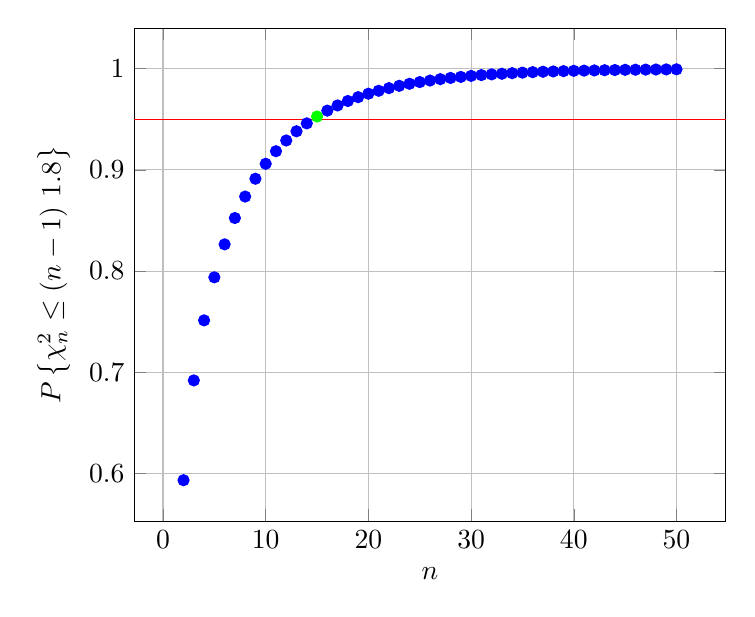
\begin{tikzpicture}
			\begin{axis}[width = 0.75\textwidth,xlabel=$n$, ylabel=$ P \left\{\chi_n^2 \leq (n-1)\ 1.8 \right\}  $, grid = both]
				
				\addplot[only marks, color = blue] plot coordinates{(2.0, 0.5934) (3.0, 0.692) (4.0, 0.7513) (5.0, 0.7938) (6.0, 0.8264) (7.0, 0.8524) (8.0, 0.8736) (9.0, 0.8912) (10.0, 0.906) (11.0, 0.9184) (12.0, 0.929) (13.0, 0.9381) (14.0, 0.9459) (16.0, 0.9585) (17.0, 0.9636) (18.0, 0.968) (19.0, 0.9718) (20.0, 0.9752) (21.0, 0.9781) (22.0, 0.9807) (23.0, 0.983) (24.0, 0.985) (25.0, 0.9867) (26.0, 0.9882) (27.0, 0.9896) (28.0, 0.9908) (29.0, 0.9918) (30.0, 0.9928) (31.0, 0.9936) (32.0, 0.9943) (33.0, 0.9949) (34.0, 0.9955) (35.0, 0.996) (36.0, 0.9965) (37.0, 0.9969) (38.0, 0.9972) (39.0, 0.9975) (40.0, 0.9978) (41.0, 0.998) (42.0, 0.9982) (43.0, 0.9984) (44.0, 0.9986) (45.0, 0.9988) (46.0, 0.9989) (47.0, 0.999) (48.0, 0.9991) (49.0, 0.9992) (50.0, 0.9993)};
				
				\addplot[only marks, color = green] plot coordinates{(15.0, 0.9527)};
			
				\draw [draw=red] (axis cs: -5,0.95) -- (axis cs: 60,0.95);
			\end{axis}
		\end{tikzpicture}
	\end{figure}

	\item Two samples with $ n_1 = 10, \sigma^2_1  = 4$ and $ n_2 = 5, \sigma^2_2  = 2$ \\
	
	\begin{subequations}
		\begin{align}
			\frac{S_1^2}{\sigma_1^2} &= \frac{\chi_9^2}{9} \qquad \frac{S_2^2}{\sigma_2^2} = \frac{\chi_4^2}{4} \nonumber \\
			%
			\frac{S_2^2}{S_1^2} &\geq 1 \qquad F_{4, 9} \geq 2 \nonumber \\
			%
			P  \left\{\frac{S_2^2}{S_1^2}  \geq 1\right\}  &= P \left\{F_{4, 9} \geq 2\right\}= 0.1782
 		\end{align}\\
	\end{subequations}
	
	\item $ n = 100, p  = 0.12$. Using the normal RV approximation with $ \mu = np = 12 $ and $ \sigma^2 = np(1-p)$ \\
	
	\begin{subequations}
		\begin{align}
			P \left\{9.5 \leq X \leq 14.5 \right\} &= P \left\{\frac{(9.5 - 12)}{\sqrt{12*0.88}} \leq Z \leq \frac{(14.5 - 12)}{\sqrt{12*0.88}} \right\} \nonumber \\
			%
			&= \Phi  \left(\frac{(14.5 - 12)}{\sqrt{12*0.88}}\right) - \Phi  \left(\frac{(9.5 - 12)}{\sqrt{12*0.88}}\right)  \nonumber \\
			%
			&= 0.5583
		\end{align}\\
	\end{subequations}

	\item Each human is a binomial RV with $ p = 0.52 $. Let $ n $ vary and check probability including continuity correction\\
	\begin{subequations}
		\begin{align}
			P \left\{ X \geq 0.5n \right\} &= P \left\{ Z \geq \frac{0.5n - 0.52n - 0.5}{\sqrt{np(1-p)}} \right\} \\
			%
			n = 10 &\to P = 0.6711 \nonumber \\
			%
			n = 100 &\to P = 0.6916 \nonumber \\
			%
			n = 1000 &\to P = 0.9028 \nonumber \\
			%
			n = 10000 &\to P = 0.99997 \nonumber 
		\end{align}\\
	\end{subequations}

	\item $ n = 300 $ men. $ c = 0.454, b = 0.284 $ \\
	\begin{subequations}
		\begin{enumerate}
			\item 			
			\begin{align}
				P \left\{X \geq 150 \right\} &= P \left\{Z \geq \frac{149.5 - 136.2}{\sqrt{300*0.454*0.546}} \right\} \nonumber \\
				%
				&= 0.0615
			\end{align} \\
			
			\item 
			\begin{align}
				P \left\{Y \leq 100 \right\} &= P \left\{Z \leq \frac{100.5 - 85.2}{\sqrt{300*0.284*0.716}} \right\} \nonumber \\
				%
				&= 0.9749
			\end{align} \\
			
		\end{enumerate}
	\end{subequations}

	\item $ n = 300 $ women. $ d = 0.256, a = 0.214 $ \\
	\begin{subequations}
		\begin{enumerate}
			\item 			
			\begin{align}
				P \left\{V \geq 60 \right\} &= P \left\{Z \geq \frac{59.5 - 76.8}{\sqrt{300*0.256*0.744}} \right\} \nonumber \\
				%
				&= 0.9889
			\end{align} \\
			
			\item 
			\begin{align}
				P \left\{U \leq 50 \right\} &= P \left\{Z \leq \frac{50.5 - 64.2}{\sqrt{300*0.214*0.786}} \right\} \nonumber \\
				%
				&= 0.0269
			\end{align} \\
			
		\end{enumerate}
	\end{subequations}

	\item More women than men rarely eat breakfast.\\
	 $ \mathbb{E}[X-Y] = -10.2 $, and $\mathrm{Var}(X-Y) = 147.4452$\\
	\begin{subequations}
		\begin{align}
			P \left\{X > Y \right\} &= P \left\{ X - Y > 0 \right\} \nonumber \\
			%
			&= P \left\{ Z > \frac{0 + 10.2}{\sqrt{147.4452}}  \right\} = 0.2005
		\end{align} \\
	\end{subequations}

	\item $ n = 1000 $ , $ p $ from the table as necessary. \\
	\begin{subequations}
		\begin{enumerate}
			\item 			
			\begin{align}
				P \left\{A \geq 500 \right\} &= P \left\{Z \geq \frac{500 - 542}{\sqrt{248.236}} \right\} \nonumber \\
				%
				&= 1 - \Phi \left( \frac{500 - 542}{\sqrt{248.236}} \right) = 0.9962
			\end{align} \\
			
			\item 
			\begin{align}
				P \left\{B > 500 \right\} &= P \left\{Z > \frac{500 - 704}{\sqrt{208.384}} \right\} \nonumber \\
				%
				&= 1 - \Phi \left( \frac{500 - 704}{\sqrt{208.384}} \right) \approx 1
			\end{align} \\
		
			\item 
			\begin{align}
				P \left\{C > 500 \right\} &= P \left\{Z > \frac{500 - 458}{\sqrt{248.236}} \right\} \nonumber \\
				%
				&= 1 - \Phi \left( \frac{500 - 458}{\sqrt{248.236}} \right) = 0.00384 \nonumber \\
				%
				P\left\{ \text{required} \right\} &= 0.00384 * 1 = 0.00384
			\end{align} \\
		
			\item 
			\begin{align}
				P \left\{D < 250 \right\} &= P \left\{Z < \frac{250 - 293}{\sqrt{207.151}} \right\} \nonumber \\
				%
				&= \Phi \left( \frac{250 - 293}{\sqrt{207.151}} \right) = 0.0014
			\end{align} \\
		
			\item 
			\begin{align}
				P \left\{E \geq 200 \right\} &= P \left\{Z \geq \frac{200 - 149}{\sqrt{126.799}} \right\} \nonumber \\
				%
				&= 1 - \Phi \left( \frac{200 - 149}{\sqrt{126.799}} \right) \approx 0
			\end{align} \\
		
			\item Let $ F = F_1 - F_2 $, with $ \mathbb{E}[F] = 31$, $ \mathrm{Var}[F] = 253.819$
			\begin{align}
				P \left\{F_1 - F_2 \geq 0 \right\} &= P \left\{Z \geq \frac{0 - 31}{\sqrt{253.819}} \right\} \nonumber \\
				%
				&= 1 - \Phi \left( \frac{0 - 31}{\sqrt{253.819}} \right) = 0.9742
			\end{align} \\
			
		\end{enumerate}
	\end{subequations}

	\item Each worker belongs to a union where $ p = 0.105 $ with $ n = 5 $. The older value of $ q = 0.201 $\\
	$ \mathbb{E}[X-Y] = -10.2 $, and $\mathrm{Var}(X-Y) = 147.4452$\\
	\begin{subequations}
		\begin{align}
			P \left\{X = 0 \right\} &= (1-p)^5 = 0.5743 \\
			%
			P \left\{Y = 0 \right\} &= (1-q)^5 = 0.3256
		\end{align} \\
	\end{subequations}

	\item $ n = 144 $ women. $ \mu = 517, \sigma = 120 $ \\
	\begin{subequations}
		\begin{enumerate}
			\item 			
			\begin{align}
				P \left\{\overline{X} > 507 \right\} &= P \left\{Z > \frac{507 - 517}{120/12} \right\} \nonumber \\
				%
				&= 1 - \Phi (-10/10) = 0.8413
			\end{align} \\
			
			\item 			
			\begin{align}
				P \left\{\overline{X} > 517 \right\} &= P \left\{Z > \frac{517 - 517}{120/12} \right\} \nonumber \\
				%
				&= 1 - \Phi (0/10) = 0.5
			\end{align} \\
		
		
			\item 			
			\begin{align}
				P \left\{\overline{X} > 537 \right\} &= P \left\{Z > \frac{537 - 517}{120/12} \right\} \nonumber \\
				%
				&= 1 - \Phi (20/10) = 0.0227
			\end{align} \\
		
			\item 			
			\begin{align}
				P \left\{\overline{X} > 550 \right\} &= P \left\{Z > \frac{550 - 517}{120/12} \right\} \nonumber \\
				%
				&= 1 - \Phi (33/10) = 0.00048
			\end{align} \\
			
		\end{enumerate}
	\end{subequations}
	
	\item $ n = 12 $ women. $ \mu = 53600, \sigma = 3200 $ \\

	\begin{subequations}
		\begin{align}
			P \left\{\overline{X} > 55000 \right\} &= P \left\{Z > \frac{55000 - 53600}{3200/\sqrt{12}} \right\} \nonumber \\
			%
			&= 0.0648
		\end{align} \\
	\end{subequations}

	\item $ n = $ is to be found. $ \mu = 100, \sigma = 30 $. Let $ Y = \sum X_i $ \\
	
	\begin{subequations}
		\begin{align}
			P \left\{Y > 2000 \right\} &= P \left\{Z > \frac{2000 - 100\ n}{30\ \sqrt{n}} \right\} \geq 0.95 \nonumber \\
			%
			\Phi \left( \frac{2000 - 100\ n}{30\ \sqrt{n}} \right) &\leq 0.05 \nonumber \\
			%
			2000 - 100\ n &\leq -1.6448 \times 30\sqrt{n} \nonumber \\
			%
			n &\geq 23
		\end{align} \\
	
	\begin{figure}[H]
		\centering
		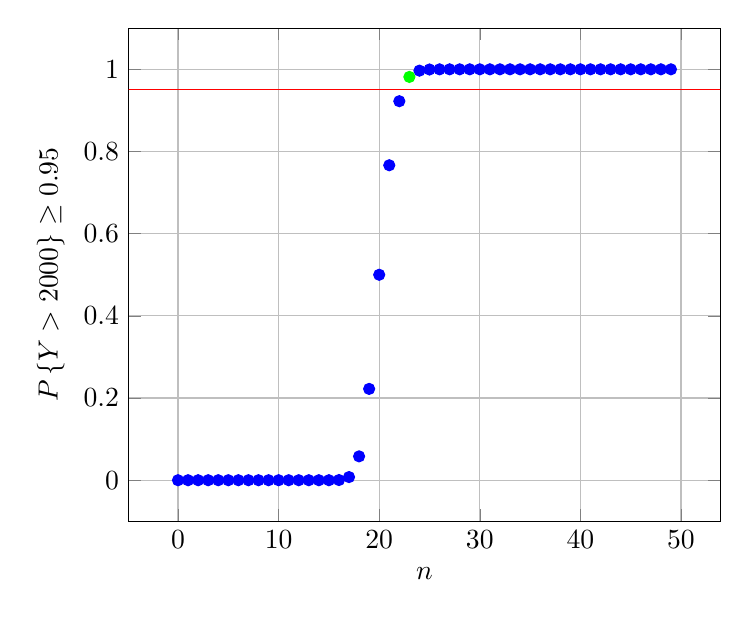
\begin{tikzpicture}
			\begin{axis}[width = 0.75\textwidth,xlabel=$n$, ylabel=$ P \left\{ Y > 2000 \right\} \geq 0.95  $, grid = both]
				
				\addplot[only marks, color = blue] plot coordinates{(0.0, 0.0) (1.0, 0.0) (2.0, 0.0) (3.0, 0.0) (4.0, 0.0) (5.0, 0.0) (6.0, 0.0) (7.0, 0.0) (8.0, 0.0) (9.0, 0.0) (10.0, 0.0) (11.0, 0.0) (12.0, 6.8833827526759706e-15) (13.0, 4.851663515381688e-11) (14.0, 4.5152443450824364e-08) (15.0, 8.413074170987578e-06) (16.0, 0.0004290603331967846) (17.0, 0.007646685515099505) (18.0, 0.058050871990274366) (19.0, 0.2222194112520176) (20.0, 0.5) (21.0, 0.7665073693266079) (22.0, 0.922390755157658) (24.0, 0.9967522068714105) (25.0, 0.9995709396668032) (26.0, 0.999956150288122) (27.0, 0.9999964472261701) (28.0, 0.9999997666572595) (29.0, 0.9999999873257626) (30.0, 0.9999999994204671) (31.0, 0.9999999999773364) (32.0, 0.9999999999992313) (33.0, 0.9999999999999771) (34.0, 0.9999999999999994) (35.0, 1.0) (36.0, 1.0) (37.0, 1.0) (38.0, 1.0) (39.0, 1.0) (40.0, 1.0) (41.0, 1.0) (42.0, 1.0) (43.0, 1.0) (44.0, 1.0) (45.0, 1.0) (46.0, 1.0) (47.0, 1.0) (48.0, 1.0) (49.0, 1.0)
				};
				
				\addplot[only marks, color = green] plot coordinates{(23.0, 0.9814718907179405)};
				
				\draw [draw=red] (axis cs: -5,0.95) -- (axis cs: 60,0.95);
			\end{axis}
		\end{tikzpicture}
	\end{figure}
	\end{subequations}
\end{enumerate}
\chapter{Parameter Estimation}


\begin{flushright}
	\textit{``Please explain in detail your reasons for choosing this prior distribution"}
\end{flushright}

Consider a distribution $ F_\theta $ from which a random sample $ \left\{X_i\right\} $ is drawn. It is an extremely common problem to estimate the vector of parameters $ \theta $ of the underlying distribution using only the information from the sample.

Estimates of these parameters can either be provided as a \textit{point} or an \textit{interval}, alongside a \textit{confidence} value associated with these estimates.

An important class of such problems is \textit{Bayesian estimation}, which involves estimating an unknown parameter only partial information about it is known.

\textbf{Maximum Likelihood Estimator} : An estimator of an unknown parameter $ \theta $ is any sample-derived statistic used to estimate its value. The observed value of an estimator is called the \textit{estimate}.

As an example consider $ n $ random samples drawn from an underlying exponential distribution whose mean is the unknown parameter $ \theta $. The joint PDF of the RVs $ \left\{X_i\right\} $, which would then be used to estimate $ \theta $ is given by

\begin{align}
	f(x_1, x_2, \dots, x_n) &= f_{x_1} (X_1)\ f_{X_2} (2_1)\ \dots\  f_{X_n} (x_n) \nonumber \\
	%
	&= \frac{1}{\theta} e^{-x_1/\theta} \ \frac{1}{\theta} e^{-x_2/\theta} \dots \ \frac{1}{\theta} e^{-x_n/\theta} \qquad x_i > 0 \nonumber \\
	%
	&= \frac{1}{\theta^n}\ \exp \left\{ \sum_{i=1}^{n} \frac{-x_i}{\theta} \right\}
\end{align}

\textit{Likelihood function} : Define $ f(x_1, x_2,\dots,x_n\ |\ \theta) $ as the joint PDF or PMF of the $ n $ random samples from an underlying distribution with unknown parameter $ \theta $. This term is the likelihood that the values $ \left\{ x_i \right\} $ will actually be observed when $ \theta $ is the true value of the parameter.

The \textit{maximum likelihood estimate} $ \widehat{\theta} $ is that value of the parameter $ \theta $ which maximizes the likelihood function. A useful computational convenience is that log likelihood also has its maximum at the same point as likelihood itself.

The algorithm usually involves identifying the likelihood function after incorporating the unknown parameter $ \theta $, taking logarithm wherever convenient, and then differentiating with respect to $ \theta $ in order to maximize the likelihood.

A sample of size $ n $ from an underlying Bernoulli distribution whose unknown mean $ p $ is to be estimated. The above procedure yields the maximum likelihood estimator of $ p $ to be the sample mean $ \sum X_i / n$.

The above problem when the underlying distribution is Poisson with rate $ \lambda $ yields the MLE as $ \widehat{\lambda} =  \sum X_i / n$.

However, for a uniform distribution on $ [0, \theta] $, the parameter is estimated by $ \widehat{\theta} = \max(\left\{X_i\right\}) $ and not by the sample mean.

The more relevant problem is with an underlying normal distribution with unknown $ \mu $ and $ \sigma $, to be estimated using a sample of size $ n $.

\begin{align}
	\widehat{\mu} = \frac{1}{n}\ \sum\limits_{i=1}^{n} x_i = \overline{X} \qquad \text{and} \qquad \widehat{\sigma} = \left[\frac{1}{n}\  \sum\limits_{i=1}^{n} (X_i - \overline{X})^2 \right] ^{1/2} \\
\end{align}

Note that $ \widehat{\sigma} $ differs from the sample standard deviation $ S $, in the denominator being $ n $ instead of $ (n-1) $.

\textit{Failure and survival rate} : Defining failure rate $ \lambda_i $ and survival rate $ s_i = 1 - \lambda_i $ for an underlying discrete distribution taking values $ i \geq 1 $,

\begin{align}
	\lambda_i &= P \left\{X = i\ |\ X > i-1\right\} = \frac{P \left\{X = i\right\}}{P\left\{X > i-1\right\}} \\
	%
	s_i &= 1 - \lambda_i = \frac{P \left\{X > i\right\}}{P\left\{X > i-1\right\}}
\end{align}

For illustration, let $ X $ denote a human's age at death. Now, failure rate is a measure of the fraction of all people surviving at least $ i-1 $ years who will die at age $ i $.

Using the relations,

\begin{align}
	P \left\{X > i\right\} &= s_1\ s_2\ \dots\ s_i \nonumber \\
	%
	P\left\{X = n\right\} &= \lambda_n\ P \left\{X > n-1\right\} = s_1\ s_2\ \dots\ s_{n-1}\ (1 - s_n) 
\end{align}

Using the above PMF for $ X $ requires estimating the survival rates $ \widehat{s_i} $. This is a simple task of looking at what fraction of the sample who reached age $ i $ one year ago are alive today.

\textbf{Interval estimates} : It is often useful to provide an interval for the estimate of a parameter along with an associated confidence value instead of just a point value. This involves looking at the probability distribution of the estimator itself.

As an example, consider the MLE of the mean of a normal RV from which a sample of size $ n $ is drawn. The MLE $ \overline{X} $ is known to have a normal distribution with mean $ \mu $ and variance $ \sigma^2 / n $.

Rearranging the sample mean to form a standard normal RV $ Z $, and using its CDF to find a $ 95\% $ confidence interval gives,

\begin{align}
	\frac{\overline{X} - \mu}{\sigma / \sqrt{n}} &\sim Z \nonumber \\
	%
	P \left\{ | \overline{X} - \mu | \leq \frac{1.96\ \sigma}{\sqrt{n}} \right\} &= 0.95 \nonumber \\
	%
	\text{with 95 \% confidence, } \mu &\in \left[ \overline{x} - \frac{1.96\ \sigma}{\sqrt{n}}, \ \overline{x} + \frac{1.96\ \sigma}{\sqrt{n}} \right]
\end{align}

The above relation states that if the sample mean $ \overline{X} = \overline{x} $, then the population mean $ \mu $ lies within this interval with $ 95\% $ confidence.

In addition to the \textit{two-sided} confidence interval for $ \mu $ above, the \textit{one-sided upper} and \textit{one-sided lower} $ 95\% $ confidence intervals for $ \mu $ are,

\begin{align}
	\mu \in \left[ \overline{x} - \frac{1.645\ \sigma}{\sqrt{n}}\ ,\  \infty \right) \qquad \text{and} \qquad \mu \in \left( -\infty\ ,\  \overline{x} + \frac{1.645\ \sigma}{\sqrt{n}} \right]
\end{align}

The factors of $ 1.96 $ and $ 1.645 $ used above were obatined using the inverse CDF of the normal distribution for $ p = 0.975 $ and $ p = 0.95 $ respectively. A different confidence interval would involve recalculating the inverse CDF and replacing the pre-factors used above.

\textit{Confidence interval for a normal mean with unknown variance} : Consider a normal RV with unknown $ \mu $ and $ \sigma $, from which a sample of size $ n $ is drawn. Since the above procedure can no longer be used to construct confidence intervals, the sample variance $ S $ is now of interest.

Using the fact that $ \sqrt{n}(\overline{X} - \mu) / S \sim t_{n-1}$, and the symmetry of the t-distribution, for some observed value of sample mean and variance $ \overline{x}, s^2 $


\begin{align}
	1 - \alpha &= P \left\{ | \overline{X} - \mu | \leq \frac{t_{\alpha/2, n-1}\ S}{\sqrt{n}} \right\}  \nonumber \\
	%
	\mu &\in \left[ \overline{x} - \frac{(t_{\alpha/2, n-1})\ s}{\sqrt{n}}, \ \overline{x} + \frac{(t_{\alpha/2, n-1})\ s}{\sqrt{n}} \right]
\end{align}

This becomes the $ 100(1-\alpha) \% $ confidence interval for $ \mu $. As $ n \to \infty $, the t-distribution reduces to the standard normal and the the new confidence interval expression reduces to the old one. It is common, but not necessary that the confidence interval when $ \sigma $ is unknown is larger than when it is known, by virtue of the t-distribution being wider than the standard normal distribution, and the general trend of $ S^2 > \sigma^2 $.

The above methods have assumed an underlying normal distribution. However, for a large enough sample size, they may be used even when the underlying PDF is not a normal RV because of the Central Limit theorem.


\textit{Monte-Carlo simulation} : The process of randomly sampling from a uniform distribution to estimate difficult integrals using the power of the central limit theorem acting on a large sample consisting of \texttt{i.i.d.} RVs.

For example, consider a set of $ n $ uniform RVs $ \left\{U_i\right\} $ in the domain $ [a,b] $ 

\begin{align}
	\theta = \int\limits_{a}^{b}\ g(x)\ \mathrm{d}x = \mathbb{E}[g(x)]
\end{align}

A new set of RVs $ \left\{X_i\right\}  = g(\left\{U_i\right\})$, which are random samples drawn from the PDF $ g(x) $, would now have sample mean and variance $ \overline{x} $ and $ s^2 $. A confidence interval for $ \mathbb{E}[g(x)] $ is now constructed using the t-distribution method described above. 

\textit{Prediction Interval} : The problem of predicting a confidence interval for the next sample $ X_{n+1} $ drawn from a normal distribution with parameters $ \mu, \sigma $ given a set of $ n $ samples already available, is similar to the above procedure.

Let $ S_n^2 $ and $ \overline{X}_n $ be the sample variance and mean using the first $ n $ samples. Since $ \overline{X}_n $ is a normal RV with mean $ \mu $ and variance $ \sigma^2 / n $, whereas $ X_{n+1} $ is also a normal RV independent of $ \overline{X}_n $ ,


\begin{align}
	\frac{X_{n+1} - \overline{X}_n}{\sigma \sqrt{1 + 1/n}} &\sim Z \nonumber \\
	%
	\frac{X_{n+1} - \overline{X}_n}{S_n \sqrt{1 + 1/n}} &\sim t_{n-1} \nonumber \\
\end{align}

Once again, this leads to the confidence intervals using the t-distribution defined above.

\textit{Confidence interval for a normal variance with unknown mean} : Using the fact that $ (n-1) S^2 / \sigma^2 \sim \chi^2_{n-1} $, the $ 100(1-\alpha) \% $ confidence interval for a sample of size $ n $ with sample variance $ S^2 = s^2 $ is calculated as,

\begin{align}
	\sigma^2 &\in \left[\ddfrac{(n-1)s^2}{\chi^2_{\alpha/2, n-1}}\ ,\ \frac{(n-1)s^2}{\chi^2_{1 - \alpha/2, n-1}}\right]
\end{align}

Note the use of $ \chi^2_{\alpha/2, n-1} $ as well as $ \chi^2_{1 - \alpha/2, n-1} $ arising from the fact that the $ \chi_n^2 $ distribution is not symmetric about its mean.

\textbf{Difference in means of two normal populations} : The problem is to estimate $ \mu_1 - \mu_2 $, where two normal RVs $ X, Y $ with means $ \mu_1, \mu_2 $ and variances $ \sigma_1^2, \sigma_2^2 $ respectively are used to generate two sets of samples $ \left\{X_1, \dots, X_n\right\} $ and $ \left\{Y_1, \dots, Y_m\right\} $.

Additionally, the sample sets $ \left\{X_i\right\}, \left\{Y_j\right\} $ are independent.

The point estimator of $ \mu_1 - \mu_2 $ is simply $ \overline{X} - \overline{Y} $, using the previous section. For an interval estimate, the distribution of $ \overline{X} - \overline{Y} $ is needed.

\begin{align}
	\overline{X} - \overline{Y} &\sim \mathcal{N}\left(\mu_1 - \mu_2\ ,\ \frac{\sigma_1^2}{n} + \frac{\sigma_2^2}{m}\right) \nonumber \\
	%
	Z &\sim \ddfrac{\overline{X} - \overline{Y} - (\mu_1 - \mu_2)}{\sqrt{\frac{\sigma_1^2}{n} + \frac{\sigma_2^2}{m}}} 
\end{align}

When the variances $ \sigma_1^2, \sigma_2^2 $ are known, the $ 100(1-\alpha)\% $ confidence interval is,

\begin{align}
	\mu_1 - \mu_2 &\in \left[ \overline{x} - \overline{y} - z_{\alpha / 2} \sqrt{\frac{\sigma_1^2}{n} + \frac{\sigma_2^2}{m}}\ ,\ \overline{x} - \overline{y} + z_{\alpha / 2} \sqrt{\frac{\sigma_1^2}{n} + \frac{\sigma_2^2}{m}} \right] 
\end{align}


Next, consider the special case where $ \sigma_1, \sigma_2 $ are unknown but happen to be equal. Now, using the sample variances $ S_1^2, S_2^2 $, and the additive property of chi-squared distributions, the \textit{pooled estimator} $ S_P^2 $ of this common variance is

\begin{align}
	S_P^2 = \frac{(n-1)\ S_1^2 + (m-1)\ S_2^2}{(n+m-2)} \nonumber
\end{align}

Rearranging the sample statistics into a t-distribution after replacing $ \sigma $ with $ S_P $,

\begin{align}
	Z &\sim \frac{\overline{X} - \overline{Y} - (\mu_1 - \mu_2)}{\sqrt{\sigma^2(1/n + 1/m)}} \nonumber \\
	%
	\chi^2_{n+m-2} &\sim (n+m-2)\ \frac{S_P^2}{\sigma^2} \nonumber \\
	%
	t_{n+m-2} &\sim \frac{\overline{X} - \overline{Y} - (\mu_1 - \mu_2)}{\sqrt{S_P^2(1/n + 1/m)}}
\end{align}

Now, the confidence interval is defined using this t-distribution as


\begin{align}
	\mu_1 - \mu_2 &\in \left[ \overline{x} - \overline{y} - t_{\alpha / 2, n+m-2}\ s_p\ \sqrt{\frac{1}{n} + \frac{1}{m}}\ ,\ \overline{x} - \overline{y} + t_{\alpha / 2, n+m-2}\ s_p\ \sqrt{\frac{1}{n} + \frac{1}{m}} \right] 
\end{align}

\textbf{Mean of a Bernoulli RV - confidence interval} : Consider a sample of size $ n $ drawn from a Bernoulli RV with parameter $ p $. The point estimate for $ p $ is simply $ \widehat{p} = \sum X_i / n $.

For an interval estimate, assume $ X = \sum X_i $ has the observed value $ x $, and define the confidence interval for $ p $ as,

\begin{align}
	Z &\sim \frac{X - np}{\sqrt{n \widehat{p} (1 - \widehat{p})}} \nonumber \\
	%
	p &\in \left[ \widehat{p} - z_{\alpha/2}\sqrt{\frac{\widehat{p}(1-\widehat{p})}{n}}\ ,\ \widehat{p} + z_{\alpha/2}\sqrt{\frac{\widehat{p}(1-\widehat{p})}{n}}  \right]
\end{align}

For a given interval of width $ b $ in the above relation, the number of samples required $ n $ is given by

\begin{align}
	b &= 2 z_{\alpha/2}\ \sqrt{\frac{\widehat{p}(1-\widehat{p})}{n}} \qquad \text{and} \qquad n = (2z_{\alpha/2})^2\  \frac{\widehat{p}(1-\widehat{p})}{b^2}
\end{align}

To guarantee a confidence interval of size $ b $ or smaller, the minimum number of samples needed is $ n^* = (Z_{\alpha/2} / b)^2 $ 

\textbf{Mean of exponential distribution - confidence interval} : Consider a set of samples $ \left\{X_1, \dots, X_n\right\} $ drawn from an exponential RV with unknown mean $ \theta $. The point estimate for $ \theta $ is just the sample mean $ \overline{X} $.

For an interval estimate, consider the following RV transformations,

\begin{align}
	\sum X_i &\sim \Gamma(n, 1/\theta) \nonumber \\
	%
	\frac{2}{\theta}\ \sum X_i &\sim \Gamma(n, 1/2) \sim \chi^2_{2n}
\end{align}

Using the above chi-squared distribution, the confidence interval for $ \theta $ is given by,

\begin{align}
	\theta \in \left[\ddfrac{2 \sum X_i}{\chi^2_{\alpha/2, 2n}}\ ,\ \ddfrac{2 \sum X_i}{\chi^2_{1 - \alpha/2, 2n}}\right]
\end{align}

\textbf{Evaluating point estimators} : The question of how good a proposed point estimator $ d(\textbf{X}) $ for a parameter $ \theta $ drawn from a sample $ \textbf{X} = \left\{X_1, \dots, X_n\right\} $ is often answered by looking at the mean squared error $ r(d, \theta) $ 

\begin{align}
	r(d, \theta) = \mathbb{E}[(d(X) - \theta)^2] 
\end{align}

Generally, there is no universal value of $ d $ that minimizes the error above for all values of $ \theta $.


\textit{Bias of an estimator} : For the definitions used above, the bias $ b_{\theta}(d) $ is expressed as,

\begin{align}
	b_\theta (d) = \mathbb{E}[d(\textbf{X})] - \theta
\end{align}

If an estimator has $ 0 $ bias for all values of $ \theta $, then it is called an \textit{unbiased} estimator of $ \theta $. For example, a weighted sum of the random samples from an unknown distribution with mean $ \theta $ is always an unbiased estimator.

\begin{align}
	\mathbb{E}\left[ \sum \lambda_i X_i \right] &= \sum \mathbb{E}[X_i]\ \lambda_i \nonumber \\
	%
	&= \theta\ \sum \lambda_i = \theta \nonumber \\
	%
	\text{if } \sum \lambda_i &= 1
\end{align}

The mean squared error of an unbiased estimator is equal to its variance.

\begin{align}
	r(d, \theta) &= \mathbb{E}[(d(\textbf{X} - \theta)^2)] = \mathbb{E}[(d(\textbf{X}) - \mathbb{E}[d(\textbf{X})])^2] \nonumber \\
	%
	&= \mathrm{Var}(d(\textbf{X}))
\end{align}

For a given parameter $ \theta $, a linear interpolant between two independent unbiased estimators $ d_1, d_2 $ is also unbiased. If $ \sigma_1^2, \sigma_2^2 $ are the respective known variances of these estimators, then this new estimator has the form 

\begin{align}
	d &= \lambda d_1 + (1-\lambda)d_2 \nonumber \\
	%
	r(d, \theta) &= \mathrm{Var}(d) = \lambda^2 \sigma_1^2 + (1-\lambda)^2 \sigma_2^2 \nonumber \\
	%
	\widehat{\lambda} &= \frac{\sigma_2^2}{\sigma_1^2 + \sigma_2^2} \qquad \text{to minimize } \qquad r(d, \theta)
\end{align}

as a generalization of the above, consider a composite estimator $ d $ made up of many independent unbiased estimators $ d_i $ each with the same mean $ \theta $ and separate variances $ \sigma^2_i $. The best construction of $ d $ would then be,

\begin{align}
	d &= \ddfrac{\sum d_i / \sigma_i^2}{\sum 1/ \sigma_i^2} \\
	%
	r(d, \theta) &= \mathrm{Var}(d) = \ddfrac{1}{\sum (1/ \sigma_i^2)}
\end{align}

For a general estimator with some nonzero bias, its mean-squared error is given by

\begin{align}
	r(d, \theta) = \mathrm{Var}(d) + b_\theta^2 (d)
\end{align}

\textbf{Bayes estimator} : Consider the special case when some information about a parameter $ \theta $ is available even before the observations $ \left\{X_i\right\} $ are obtained. This is called the \textit{prior distribution} of $ \theta $.

However, once the set of $ n $ random variables $ \left\{X_i = x_i\right\} $ have been observed, it is possible to update the prior PDF $ p(\theta) $ using this new information to yield the \textit{posterior distribution} $ f(\theta\ |\ x_1, \dots, x_n) $.

The update procedure uses the \textit{likelihood} $ f(x\ |\ \theta) $ and Bayes' theorem to calcuate the posterior distribution.

\begin{align}
	f(\theta\ |\ x_1, \dots, x_n) &= \frac{f(\theta, x_1, \dots, x_n)}{f(x_1, \dots, x_n)} \nonumber \\
	%
	&= \ddfrac{f(x_1, \dots, x_n\ |\ \theta)\ p(\theta)}{\int\limits f(x_1, \dots, x_n\ |\ \theta)\ p(\theta)\  \mathrm{d}\theta}
\end{align}

The Bayes estimator is simply the mean of the posterior distribution $ \mathbb{E}[\theta\ |\ X_1, \dots, X_n] $, as it minimizes the expected square error in estimating $ \theta $. If the set of RVs take on the values $ \left\{X_i = x_i\right\} $,

\begin{align}
	\mathbb{E}[\theta\ |\ X_1, \dots, X_n] &= \int\limits \theta\ f(\theta\ |\ x_1, \dots, x_n)\ \mathrm{d}\theta
\end{align}

As an example, consider a set of independent normal RVs $ \left\{X_i\right\} $ each with unknown mean $ \theta $ and known variance $ \sigma_0^2 $. Now, suppose the prior distribution of $ \theta $ is itself normal with known parameters $ (\mu, \sigma^2) $. The Bayes estimator of $ \theta $ happens to be a normal RV with

\begin{align}
	\mathbb{E}[\theta\ |\ X_1, \dots, X_n] &= \left(\frac{n\sigma^2}{n\sigma^2 + \sigma_0^2}\right)\ \overline{X} + \left(\frac{\sigma_0^2}{n\sigma^2 + \sigma_0^2}\right)\ \mu \\
	%
	\mathrm{Var}(\theta\ |\ X_1, \dots, X_n) &= \frac{\sigma^2 \sigma_0^2}{n\sigma^2 + \sigma_0^2}
\end{align}

Choosing a normal RV for the prior distribution is justifiable if


\begin{itemize}
	\item The parameter $ \theta $ is likely to be close to a value $ \mu $.
	
	\item $ \theta $ is just as likely to be a certain distance away from $ \mu $ whether larger or smaller. This justifies a symmetric distribution about $ \mu $.
	
	\item There exists some number $ \sigma $ such that \\
	\begin{align}
		P\left\{|\theta - \mu| \leq z_{\alpha/2}\right\} = 1- \alpha \nonumber
 	\end{align}
 	for some conventional choice of $ \alpha $ such as $ 0.05 $. 
\end{itemize}


For an interval estimate of $ \theta $, say in the interval $ [a,b] $, with probability $ 1-\alpha $ use

\begin{align}
	\int\limits_a^b \ f(\theta\ |\ x_1, \dots, x_n)\ \mathrm{d}\theta = 1 - \alpha
\end{align}








\newpage


%\chapter*{Exercises C7}

\begin{enumerate}
	
	\item \begin{subequations}
		To determine MLE of $ \theta $, first find the joint PDF $ f(x_1, x_2, \dots, x_n) $ \\
			\begin{align}
				f(x_1, x_2, \dots, x_n | \theta) &= \prod_{i=1}^{n} \exp(\theta-x_i) \qquad \forall\ x_i \geq \theta \nonumber \\
				%
				&= \exp \left[ \sum\limits_{i=1}^{n} (\theta - x_i) \right] = \exp \left[n\theta - \sum x_i\right] \nonumber \\
				%
				\log (f) &= n\theta - \sum x_i		
			\end{align}
		This is maximised when $ \theta $ is maximised, but $ \theta \leq x_i\ \forall i \in \{1,\dots, n\} $.
		Thus, $ \widehat{\theta} = \min(\{x_i\}) $ \\
	\end{subequations}
	
	\item \begin{subequations}
		\begin{align}
		f(x) &= 0.5\ \exp\left(-|x- \theta|\right) \qquad \forall\ x \in \mathbb{R} \nonumber \\
		%
		f(x_1, x_2, \dots, x_n | \theta) &= \frac{1}{2^n}\ \exp\left[ \sum\limits_{i=1}^{n} -|x_i - \theta| \right] \nonumber \\
		%
		\log (f) &= -n\log (2) - \sum\limits_{i=1}^{n} |x_i - \theta| 
	\end{align}
	\end{subequations} \\
	
	
	$ \sum |x_i - \theta| $ is total absolute error. This is minimized by $ \widehat{\theta} = \mathrm{median}(x_1, \dots, x_n)$\\
	
	\item $ \mu $ is known, find MLE of $ \sigma^2 $. To find joint PDF and thus likelihood function,
	
	\begin{subequations}
	\begin{align}
		f(x_1, x_2, \dots, x_n | \sigma^2) &= \left(\frac{1}{\sqrt{2\pi\sigma^2}}\right)^n\ \exp \left[\sum\limits_{i=1}^{n}\ \frac{-(x_i - \mu)^2}{2\sigma^2}\right] \nonumber \\
		%
		\log(f) &= -(n/2)\ \log(2\pi) - n\ \log(\sigma) - \left[\sum\limits_{i=1}^{n}\ \frac{(x_i - \mu)^2}{2\sigma^2}\right] \\
		%
		\frac{\mathrm{d}}{\mathrm{d} \sigma^2}\ \log(f) &= 0 \nonumber \\
		%
		0 &= -\ddfrac{n}{2\sigma^2} + \frac{\sum (x_i - \mu)^2}{2\sigma^4} \nonumber \\
		%
		\widehat{\sigma}^2 &= \frac{\sum (x_i - \mu)^2}{n} \\
		%
		\mathbb{E}\left[\widehat{\sigma^2}\right] &= 1/n \sum \mathbb{E}[(x_i - \mu)^2] = \sigma^2
	\end{align}
	\end{subequations}
	\item Pareto density function with parameters $ (a, \lambda) $. Constraint on $ a $ is that $ a \leq \min({x_i}) $.
	Let $ y = \prod\limits_{i=1}^{n} x_i $
	
	\begin{subequations}
	\begin{align}
		f(x) &= \lambda a^\lambda x^{-(\lambda+1)} \qquad \forall\ x \geq a \nonumber \\
		%
		f(x_1, x_2, \dots, x_n | a, \lambda) &= \lambda^n\ a^{n\lambda}\ y^{-(\lambda + 1)} \\
		%
		\widehat{a} &= \min(\{x_i\}) \\
		%
		\frac{\mathrm{d}}{\mathrm{d} \lambda}\ (\log f) &= \frac{n}{\lambda} + n \log (a) - \log (y) \nonumber \\
		%
		\widehat{\lambda} &= \frac{n}{\log (y) - n \log (a)}
	\end{align}
	\end{subequations}

	\item Given the three sets of RVs, with means $ \mu_1, \mu_2, (\mu_1 + \mu_2) $, and common variance $ \sigma^2 $.
	
	\begin{subequations}
	\begin{align}
		G_i(\mu_1, \mu_2) &= (x_i - \mu_1)^2 + (y_i - \mu_2)^2 + (w_i - \mu_1 - \mu_2)^2 \nonumber \\
		%
		f(x_1, y_1,w_1, \dots, x_n, y_n, w_n | \mu_1, \mu_2) &= \left(\frac{1}{\sqrt{2\pi\sigma^2}}\right)^{3n}\ \exp \left[-\sum\limits_{i=1}^{n}\ \frac{G_i(\mu_1, \mu_2)}{2\sigma^2}\right] \nonumber \\
		%
		\log(f) &= -(3n/2)\ \log(2\pi) - 3n\ \log(\sigma) \nonumber \\
		%
		&- \left[\sum\limits_{i=1}^{n}\ \frac{G_i(\mu_1, \mu_2)}{2\sigma^2}\right] \\
		%
		\frac{\mathrm{d}}{\mathrm{d} \mu_1}\ \log(f) &= 0 \nonumber \\
		%
		0 &= \frac{1}{\sigma^2}\ \sum\limits_{i=1}^{n}\ (x_i - \mu_1) + (w_i - \mu_1 - \mu_2) \nonumber \\
		%
		\overline{X} + \overline{W} &= (2\widehat{\mu_1} + \widehat{\mu_2}) \\
		%
		\overline{Y} + \overline{W} &= (\widehat{\mu_1} + 2\widehat{\mu_2}) \nonumber \\
		%
		\widehat{\mu_1} = \frac{2\overline{X} - \overline{Y} + \overline{W}}{3} \qquad &\text{and} \qquad \widehat{\mu_2} = \frac{-\overline{X} + 2\overline{Y} + \overline{W}}{3}
	\end{align}
	\end{subequations}
	
	\item The sample mean and variance of $ Y = \log(X) $ is calculated as $ \overline{Y} = 3.7319,\ S_Y^2 = 0.0508 $.
	
	\begin{subequations}
	\begin{align}
		P \left\{ D \geq v \right\} &= 0.01 \nonumber \\
		%
		P \left\{ \frac{Y - \overline{Y}}{S_Y} \geq z_{0.01}\right\} &= 0.01 \nonumber \\
		%
		Y &\geq 9.8 \qquad \to \qquad X \geq 18041.35	
	\end{align}
	\end{subequations}

	Thus, a 100-year flood has a discharge of $ 18041 $.
	
	\item $ X $ is a log-normal RV. Let $ Y = \log X $. The moment generating function leads to mean and variance.
	\begin{subequations}
	\begin{enumerate}
		\item Using the MGF of $ Y $,
		\begin{align}
			\phi_Y(t) &= \exp \left( \mu t  + \frac{\sigma^2 t^2}{2}\right) \nonumber \\
			%
			\mathbb{E}[e^{Yt}] &= \mathbb{E}[X^t] \nonumber \\
			%
			\mathbb{E}[X] &= \exp \left(\mu + \frac{\sigma^2}{2}\right)
		\end{align}
	
		\item To find variance, set $ t = 2 $,
		\begin{align}
			\mathbb{E}[X^2] &= \exp \left(2\mu + 2\sigma^2\right) \nonumber \\
			%
			\mathrm{Var}(X) &= \exp \left(2\mu + 2\sigma^2\right) - \exp \left(2\mu + \sigma^2\right)
		\end{align}
	
		\item Calculating mean travel time using the above formulae,
		find $\mu =  \overline{Y} = 45.4 $ and $ \sigma^2 = S_Y^2 = 131.82 $.
		
		\begin{align}
			\mathbb{E}[X] &= \exp \left(\mu + 0.5\sigma^2\right) = 45.56
		\end{align}
		
	\end{enumerate}
	\end{subequations}

	\item The sample mean and variance of $ Y = X + \mathcal{N} (0, 0.1^2) $ is calculated as
	 $ \overline{Y} = 3.1502,\ S_Y = 0.0092 $.
	
	\begin{subequations}
		\begin{align}
			Y &\sim \mathcal{N}(X, 0.1^2) \nonumber \\
			%
			\text{95\% confidence interval is } X &\in \left(\overline{Y} \pm\frac{\sigma\ z_{0.025}}{\sqrt{n}}\right) \nonumber \\
			%
			&= 3.1502 \pm 0.08765 = [3.0625, 3.2378] \\
			%
			\text{99\% confidence interval is } X &\in \left(\overline{Y} \pm\frac{\sigma\ z_{0.005}}{\sqrt{n}}\right) \nonumber \\
			%
			&= 3.1502 \pm 0.11519 = [3.0350, 3.2654]
		\end{align}
	\end{subequations}
	
	\item The sample mean and variance of $ Y \sim \mathcal{N} (\mu, 0.08^2) $ is calculated as
	$ \overline{Y} = 11.48$.
	
	\begin{subequations}
		\begin{align}
			\text{95\% confidence interval is } \mu &\in \left(\overline{Y} \pm\frac{\sigma\ z_{0.025}}{\sqrt{n}}\right) \nonumber \\
			%
			&= 3.1502 \pm 0.04958 = [11.4304, 11.5296] \\
			%
			\text{95\% upper confidence interval is } X &\geq \overline{Y} - \frac{\sigma\ z_{0.05}}{\sqrt{n}} \nonumber \\
			%
			&= 3.1502 - 0.04161 = [11.4384, \infty) \nonumber \\
			%
			\text{95\% lower confidence interval is } X &\leq \overline{Y} + \frac{\sigma\ z_{0.05}}{\sqrt{n}} \nonumber \\
			%
			&= 3.1502 + 0.04161 = (-\infty, 11.5216]
		\end{align}
	\end{subequations}

	\item The sample mean and variance of $ Y \sim \mathcal{N} (\mu, 11.3^2) $ is given as
	$ \overline{Y} = 74.6, n = 81$.
	
	\begin{subequations}
		\begin{align}
			\text{95\% confidence interval is } \mu &\in \left(\overline{Y} \pm \frac{\sigma\ z_{0.025}}{\sqrt{n}}\right) \nonumber \\
			%
			&= 74.6 \pm 2.0652 = [72.5348, 76.6652] 
		\end{align}
	\end{subequations}

	\item $ \overline{X_n} $ is a the mean of the first $ n $ samples. $ \sigma^2 = 1 $ \\
	\begin{subequations}
		\begin{enumerate}
			\item Find the distribution of $ X_{n+1} - \overline{X}_n $,
			\begin{align}
				\overline{X_n} &\sim \mathcal{N}(\mu, \sigma^2/n) \nonumber \\
				%
				X_{n+1} &\sim \mathcal{N}(\mu, \sigma^2) \nonumber \\
				%
				X_{n+1} - \overline{X}_n &\sim \mathcal{N}(0,1 + 1/n)
			\end{align}
			
			\item $ \overline{X_n} = 4 $,
			\begin{align}
				\text{90\% confidence interval is } X_{n+1} &\in \left(\overline{X_n} \pm \sqrt{1 + 1/n}\ z_{0.05}\right)
			\end{align}
			
		\end{enumerate}
	\end{subequations}

	\item The sample mean $ \mu $ is unknown and variance is known to be $ \sigma^2 $. For a $ 100(1-\alpha) $ lower confidence interval \\
	
	\begin{subequations}
		\begin{align}
			\frac{\overline{X} - \mu}{\sigma / \sqrt{n}} &\sim Z \nonumber \\
			%
			P \left\{\frac{\overline{X} - \mu}{\sigma / \sqrt{n}} > z_\alpha\right\} &= 1 - \alpha\\
			%
			\mu &< \overline{X} + \frac{z_\alpha\ \sigma}{\sqrt{n}} \nonumber \\
			%
			\mu &\in \left(-\infty\ ,\ \overline{X} + \frac{z_\alpha\ \sigma}{\sqrt{n}}\right]
		\end{align}
	\end{subequations}
	
	\item The sample mean $ \mu $ is unknown and variance is known to be $ \sigma = 0.2 $. The 99\% two-sided confidence interval is
	$ \overline{Y} = 1.2, n = 20$.
	\begin{subequations}
		\begin{align}
			\mu &\in \left(\overline{Y} \pm \frac{\sigma\ z_{0.005}}{\sqrt{n}}\right) \nonumber \\
			%
			&= 1.2 \pm 0.1152 = [1.0848, 1.3152] 
		\end{align}
	\end{subequations}

	\item Using problem 13 data but with $ \sigma $ unknown and $ S^2 = 0.04 $. For a 99\% confidence interval, use $ \alpha = 0.01 $, $ \overline{Y} = 1.2, n = 20$.
	\begin{subequations}
		\begin{align}
			\mu &\in \left[ \overline{Y} - \frac{(t_{\alpha/2, n-1})\ s}{\sqrt{n}}, \ \overline{Y} + \frac{(t_{\alpha/2, n-1})\ s}{\sqrt{n}} \right] \nonumber \\
			%
			\mu &\in 1.2 \pm 0.1279 = [1.0720, 1.3279]
		\end{align}
	\end{subequations}

	\item Using problem 14 data to find one-sided 99\% confidence interval.
	\begin{subequations}
		\begin{align}
			\mu &\in \left(-\infty\ , \ \overline{Y} + \frac{(t_{\alpha, n-1})\ s}{\sqrt{n}} \right] \nonumber \\
			%
			c &= 1.2 + 0.1136 = 1.31357
		\end{align}
	\end{subequations}
	
	\item First perform a sub-sampling with $ m = 30$ and use it to find the required sample size $ n $. Normal RV with both mean and variance unknown.
	\begin{subequations}
		\begin{enumerate}
			\item Using $ m = 30 $, this subsample has variance $ S^2_m $. The interval width will then be\\
			\begin{align}
				b = 2t_{\alpha/2, m-1}\ \frac{S_m}{\sqrt{m}}
			\end{align}
			
			\item For large $ n $, this can be approximated to a standard normal RV $ Z $.
			\begin{align}
				A = 2z_{\alpha/2}\ \frac{S_m}{\sqrt{n}}
			\end{align}
	Solving for $ n $ gives the size of the full sample.
		\end{enumerate}
	\end{subequations}

	\item $ \sigma $ unknown and $ S = 6.9576 $. For a 95\% confidence interval, use $ \alpha = 0.01 $, $ \overline{Y} = 333.9958, n = 24$. Using a t-distribution with $ 23 $ DOF, which yields slightly larger intervals than a standard normal RV\\
	\begin{subequations}
		\begin{align}
			\mu &\in \left[ \overline{Y} - \frac{(t_{\alpha/2, n-1})\ s}{\sqrt{n}}, \ \overline{Y} + \frac{(t_{\alpha/2, n-1})\ s}{\sqrt{n}} \right] \nonumber \\
			%
			\mu &\in 333.9958 \pm 2.9379 = [331.0579, 336.9338] \qquad \text{95\% confidence} \nonumber \\
			%
			\mu &\in 333.9958 \pm 3.9870 = [330.0088, 337.9828] \qquad \text{99\% confidence} 
		\end{align}
	\end{subequations}

	\item $ \sigma $ unknown and $ S = 10.2127 $, $ \overline{Y} = 133.22, n = 18$. Using a t-distribution with $ 17 $ DOF, which yields slightly larger intervals than a standard normal RV\\
	\begin{subequations}
		\begin{align}
			\mu &\in \left[ \overline{Y} - \frac{(t_{\alpha/2, n-1})\ s}{\sqrt{n}}, \ \overline{Y} + \frac{(t_{\alpha/2, n-1})\ s}{\sqrt{n}} \right] \nonumber \\
			%
			\mu &\in 333.9958 \pm 4.3125 = [128.9097, 137.5347] \qquad \text{95\% confidence} \nonumber \\
			%
			\mu &\in \left(-\infty\ ,\  137.5312\right] \qquad \text{lower 95\% confidence} \nonumber \\
			%
			\mu &\in \left[128.9133\ ,\ \infty\right) \qquad \text{upper 95\% confidence}
		\end{align}
	\end{subequations}

	\item $ \sigma $ unknown and $ S = 22 $, $ \overline{Y} = 222, n = 9$. Using a t-distribution with $ 8 $ DOF, which yields slightly larger intervals than a standard normal RV\\
	\begin{subequations}
		\begin{align}
			\mu &\in \left[ \overline{Y} - \frac{(t_{\alpha, n-1})\ s}{\sqrt{n}}, \infty \right) \nonumber \\
			%
			\mu &\in \left[208.363\ ,\ \infty\right) \qquad \text{upper 95\% confidence}
		\end{align}
	\end{subequations}

	\item $ \sigma $ unknown and $ S = 800 $, $ \overline{Y} = 2200, n = 18$. Using a t-distribution with $ 15 $ DOF, which yields slightly larger intervals than a standard normal RV\\
	\begin{subequations}
		\begin{align}
			\mu &\in \left[ \overline{Y} - \frac{(t_{\alpha/2, n-1})\ s}{\sqrt{n}}, \ \overline{Y} + \frac{(t_{\alpha/2, n-1})\ s}{\sqrt{n}} \right] \nonumber \\
			%
			\mu &\in 333.9958 \pm 350.61 = [1849.3899, 2550.6101] \qquad \text{90\% confidence}
		\end{align}
	\end{subequations}

	\item $ \sigma $ unknown and $ S = 16 $, $ \overline{Y} = 320, n = 100$. Using a t-distribution with $ 99 $ DOF, which yields slightly larger intervals than a standard normal RV\\
	\begin{subequations}
		\begin{align}
			\mu &\in \left[ \overline{Y} - \frac{(t_{\alpha/2, n-1})\ s}{\sqrt{n}}, \ \overline{Y} + \frac{(t_{\alpha/2, n-1})\ s}{\sqrt{n}} \right] \nonumber \\
			%
			\mu &\in 320 \pm 3.1747 = [316.8252, 323.1747] \qquad \text{95\% confidence}
		\end{align}
	\end{subequations}
	
	\item $ \sigma $ unknown and $ S = 15.4 $, $ \overline{Y} = 330.2, n = 20$. Using a t-distribution with $ 19 $ DOF, which yields slightly larger intervals than a standard normal RV\\
	\begin{subequations}
		\begin{align}
			\mu &\in \left[ \overline{Y} - \frac{(t_{\alpha/2, n-1})\ s}{\sqrt{n}}, \ \overline{Y} + \frac{(t_{\alpha/2, n-1})\ s}{\sqrt{n}} \right] \nonumber \\
			%
			\mu &\in 330.2 \pm 7.2074 = [322.9926, 337.4074] \qquad \text{95\% confidence} \nonumber \\
			%
			\mu &\in 330.2 \pm 9.8517 = [320.3482, 340.0517] \qquad \text{99\% confidence}
		\end{align}
	\end{subequations}

	\item $ \sigma $ unknown and $ S = 840 $, $ \overline{Y} = 1220, n = 300$. Using a t-distribution with $ 299 $ DOF, which yields slightly larger intervals than a standard normal RV\\
	\begin{subequations}
		\begin{align}
			\mu &\in \left[ \overline{Y} - \frac{(t_{\alpha/2, n-1})\ s}{\sqrt{n}}, \ \overline{Y} + \frac{(t_{\alpha/2, n-1})\ s}{\sqrt{n}} \right] \nonumber \\
			%
			\mu &\in 1220 \pm 95.4395 = [1124.5605, 1315.4395] \qquad \text{95\% confidence} 
		\end{align}
	\end{subequations}

	\item from Problem 23,
	\begin{subequations}
		\begin{align}
			\mu &\in \left(-\infty\ ,\  \overline{Y} - \frac{(t_{\alpha, n-1})\ s}{\sqrt{n}} \right] \nonumber \\
			%
			\mu &\in \left(-\infty\ ,\ 1282.2896  \right] \qquad \text{upper 90\% confidence} \nonumber \\
			%
			v &= 1282.2896
		\end{align}
	\end{subequations}
	
	\item confidence interval for $ \mu $ when $ \sigma^2 $ is unknown. Using the sample mean and sample variance $ \overline{X}, S^2 $, and the observations for these statistics $ \overline{x}, s^2 $\\
	\begin{subequations}
		\begin{align}
			\frac{\overline{X} - \mu}{S/\sqrt{n}} &\sim t_{n-1} \nonumber \\
			%
			P \left\{ \frac{\overline{X} - \mu}{S/\sqrt{n}} > -t_{\alpha, n-1}\right\} &= 1 - \alpha \nonumber \\
			%
			\mu \in \left( -\infty\ ,\ \overline{x} + \frac{t_{\alpha, n-1}\ s}{\sqrt{n}} \right]
		\end{align}
	\end{subequations}
	
	\item $ \sigma $ unknown and $ S = 104.3435 $, $ \overline{Y} = 2062.75, n = 20$. Using a t-distribution with $ 19 $ DOF, which yields slightly larger intervals than a standard normal RV\\
	\begin{subequations}
		\begin{align}
			\mu &\in \left[ \overline{Y} - \frac{(t_{\alpha/2, n-1})\ s}{\sqrt{n}}, \ \overline{Y} + \frac{(t_{\alpha/2, n-1})\ s}{\sqrt{n}} \right] \nonumber \\
			%
			\mu &\in 2062.75 \pm 48.8343 = [2013.9157, 2111.5843] \qquad \text{95\% confidence} \nonumber \\
			%
			\mu &\in 2062.75 \pm 66.7511 = [1995.9989, 2129.5011] \qquad \text{99\% confidence} \nonumber \\
			%
			v &= 2022.41
		\end{align}
	\end{subequations}

	\item $ \sigma $ unknown and $ S = 8.6879 $, $ \overline{Y} = 98.67, n = 20$. Using a t-distribution with $ 19 $ DOF, which yields slightly larger intervals than a standard normal RV\\
	\begin{subequations}
		\begin{align}
			\mu &\in \left[ \overline{Y} - \frac{(t_{\alpha/2, n-1})\ s}{\sqrt{n}}, \ \overline{Y} + \frac{(t_{\alpha/2, n-1})\ s}{\sqrt{n}} \right] \nonumber \\
			%
			\mu &\in 98.67 \pm 4.0660 = [94.6039, 102.7360] \qquad \text{95\% confidence} 
		\end{align}
	\end{subequations}

	\item $ \sigma $ unknown and $ S = 0.02944 $, $ \overline{Y} = 0.55, n = 10$. Using a t-distribution with $ 9 $ DOF, which yields slightly larger intervals than a standard normal RV\\
	\begin{subequations}
		\begin{align}
			\mu &\in \left[ \overline{Y} - \frac{(t_{\alpha/2, n-1})\ s}{\sqrt{n}}, \ \overline{Y} + \frac{(t_{\alpha/2, n-1})\ s}{\sqrt{n}} \right] \nonumber \\
			%
			\mu &\in 0.55 \pm 0.02106 = [0.52894, 0.57106] \qquad \text{95\% confidence} 
		\end{align}
	\end{subequations}

	\item \begin{subequations}
		To find the PMF of $ N $, look at the CDF of $ N $ first. $ \mathbb{E}[U_i] = 1/2, \mathrm{Var}(U_i) = 1/12 $\\
	Consider $ S_n = U_1 + \dots + U_n $ and some. This is the $ n $ dimensional simplex problem.
	
	When finding the area of the $ n $-simplex, 
	
	Begin by proving the recursion formula for the volume of an $ n $ dimensional simplex. Let $ {X_i} $ be such that uniform RV $ X_i \in [0, 1] $ and the constraint $ \sum x_i  \leq 1$.
	
			Using analytical methods to find the exact asymptotic value of $ \mathbb{E}[X] $
			\begin{align}
				P\{S_1 \leq 1\} = A_1 &= P\{X_1 \leq 1\} = 1 \nonumber \\
				%
				P\{S_2 \leq 1\} = A_2 &= \int\limits_{0}^{1} \int\limits_{0}^{1-y} \mathrm{d}x\ \mathrm{d}y = \frac{1}{2}\\
				%
				P\{S_3 \leq 1\} = A_3 &= \int\limits_{0}^{1} (1-z)^2\ A_2\ \mathrm{d}z = \frac{A_2}{3} = \frac{1}{6}\\
				%
				P\{S_n \leq 1\} = A_n &= \int_{0}^{1} (1-x_n)^{n-1}\ A_{n-1}\ \mathrm{d}x_n = \frac{A_{n-1}}{n}		
			\end{align}
		
			The above factor of $ (1-x_n)^{n-1} $ arises as a result of all of the other $ n-1 $ dimensions being scaled down by a factor of $ 1-x_n $ when $ x_n > 0 $. From recursion, $ A_n = 1/n!$\\
			
			Now, using the above as a CDF of $ N $, then its PDF and expected value\\
			\begin{align}
				P\{N \leq n\} &= 1 - P\{N > n\} = A_n = 1 - \frac{1}{n!} \nonumber \\
				%
				P\{N = n\} &= P\{N \leq n\} - P\{N \leq n-1\} = \frac{n-1}{n!} \\
				%
				\mathbb{E}[X] &= \sum\limits_{i=1}^{\infty} i\ P\{N = i\} = \sum\limits_{i=0}^{\infty} \frac{1}{i!} = e 
			\end{align}
			
		
			Thus, the expected value of $ X $ converges to the natural logarithm $ e $.
		
			Using a Monte-Carlo simulation with $ n = k^2 \ \forall\ k \in [4, 99]$ \\
			
		\begin{figure}[H]
			\centering
			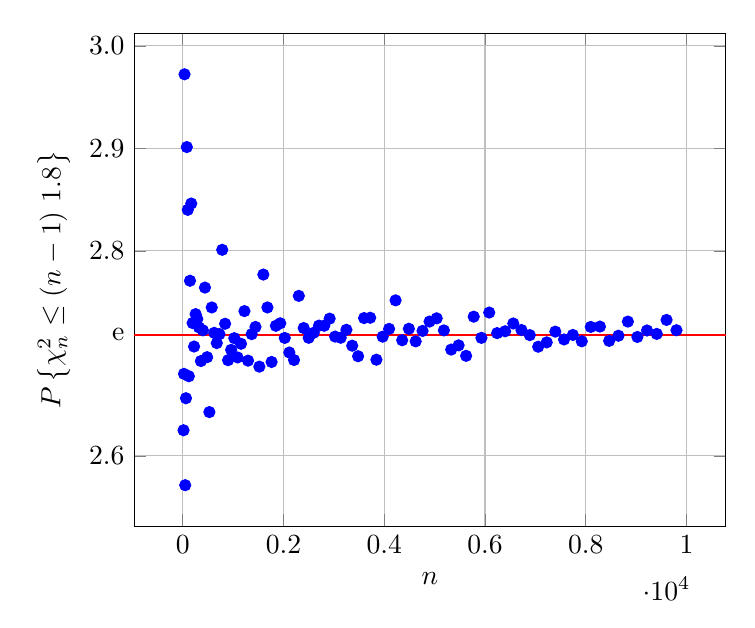
\begin{tikzpicture}
				\begin{axis}[width = 0.75\textwidth,xlabel=$n$, ylabel=$ P \left\{\chi_n^2 \leq (n-1)\ 1.8 \right\}  $, grid = both, ytick = {2.4, 2.6, e, 2.8, 2.9, 3.0}, yticklabels = {2.4, 2.6, e, 2.8, 2.9, 3.0}]
					
					\addplot[only marks, color = blue] plot coordinates{(16, 2.625) (25, 2.68) (36, 2.9722222222222223) (49, 2.5714285714285716) (64, 2.65625) (81, 2.9012345679012346) (100, 2.84) (121, 2.677685950413223) (144, 2.7708333333333335) (169, 2.8461538461538463) (196, 2.729591836734694) (225, 2.7066666666666666) (256, 2.73828125) (289, 2.7335640138408306) (324, 2.7253086419753085) (361, 2.6925207756232687) (400, 2.7225) (441, 2.764172335600907) (484, 2.696280991735537) (529, 2.6427221172022684) (576, 2.7447916666666665) (625, 2.72) (676, 2.710059171597633) (729, 2.718792866941015) (784, 2.8010204081632653) (841, 2.728894173602854) (900, 2.6933333333333334) (961, 2.7034339229968785) (1024, 2.71484375) (1089, 2.6960514233241506) (1156, 2.709342560553633) (1225, 2.7412244897959184) (1296, 2.692901234567901) (1369, 2.718772826880935) (1444, 2.7257617728531858) (1521, 2.6870479947403023) (1600, 2.776875) (1681, 2.744794765020821) (1764, 2.691609977324263) (1849, 2.7268793942671716) (1936, 2.729338842975207) (2025, 2.7150617283950615) (2116, 2.700850661625709) (2209, 2.6935264825712992) (2304, 2.756076388888889) (2401, 2.724698042482299) (2500, 2.7152) (2601, 2.7201076509034987) (2704, 2.7270710059171597) (2809, 2.7269490922036312) (2916, 2.7338820301783264) (3025, 2.7163636363636363) (3136, 2.7152423469387754) (3249, 2.7229916897506925) (3364, 2.7074910820451845) (3481, 2.697213444412525) (3600, 2.7344444444444442) (3721, 2.734748723461435) (3844, 2.693808532778356) (3969, 2.7163013353489545) (4096, 2.723876953125) (4225, 2.751715976331361) (4356, 2.7128099173553717) (4489, 2.7239919803965247) (4624, 2.7117214532871974) (4761, 2.7219071623608486) (4900, 2.7310204081632654) (5041, 2.734179726244793) (5184, 2.72241512345679) (5329, 2.70369675361231) (5476, 2.70781592403214) (5625, 2.6976) (5776, 2.735803324099723) (5929, 2.7151290268173387) (6084, 2.7398093359631823) (6241, 2.7197564492869732) (6400, 2.7215625) (6561, 2.7291571406797743) (6724, 2.7227840571088637) (6889, 2.717811003048338) (7056, 2.7064909297052155) (7225, 2.710726643598616) (7396, 2.721200648999459) (7569, 2.7135685031047694) (7744, 2.71797520661157) (7921, 2.711778815806085) (8100, 2.7258024691358025) (8281, 2.7261200338123417) (8464, 2.7121928166351608) (8649, 2.717192739044976) (8836, 2.730986871887732) (9025, 2.71601108033241) (9216, 2.7223307291666665) (9409, 2.7189924540333723) (9604, 2.7326114119117033) (9801, 2.722579328639935)};
					
					\draw [thick, draw=red,] (axis cs: -1000, e ) -- (axis cs: 11000,  e );
				\end{axis}
			\end{tikzpicture}
		\end{figure}
	\end{subequations}

	\item $ \sigma $ unknown and $ S = 3.9799 $, $ \overline{Y} = 11.5666, n = 30$. Using a t-distribution with $ 29 $ DOF, which yields slightly larger intervals than a standard normal RV\\
	\begin{subequations}
		\begin{align}
			\mu &\in \left[ \overline{Y} - \frac{(t_{\alpha/2, n-1})\ s}{\sqrt{n}}, \ \overline{Y} + \frac{(t_{\alpha/2, n-1})\ s}{\sqrt{n}} \right] \nonumber \\
			%
			\mu &\in 11.5666 \pm 1.4861 = [10.0805, 13.0528] \qquad \text{95\% confidence} 
		\end{align}
	\end{subequations}
	
	\item $ \sigma $ unknown and $ S = 9400 $, $ \overline{Y} = 90450, n = 16$. Using a t-distribution with $ 15 $ DOF, which yields slightly larger intervals than a standard normal RV\\
	\begin{subequations}
		\begin{align}
			\mu &\in \left[ \overline{Y} - \frac{(t_{\alpha/2, n-1})\ s}{\sqrt{n}}, \ \overline{Y} + \frac{(t_{\alpha/2, n-1})\ s}{\sqrt{n}} \right] \nonumber \\
			%
			\mu &\in 90450 \pm 5008.9064 = [85441.0936, 95458.9064] \qquad \text{95\% confidence} 
		\end{align}
	\end{subequations}

	\item Find the mean squared error of the predictor $ \overline{X} $,
	\begin{subequations}
		\begin{align}
			\overline{X_n} &\sim \mathcal{N}(\mu, \sigma^2/n) \nonumber \\
			%
			X_{n+1} &\sim \mathcal{N}(\mu, \sigma^2) \nonumber \\
			%
			Y = X_{n+1} - \overline{X_n} &\sim \mathcal{N}(0, \sigma^2\ (1+1/n))\nonumber \\
			%
			\mathbb{E}[Y^2] &= \mathrm{Var}(Y) + \left(\mathbb{E}[Y]\right)^2 = \sigma^2\ \left(1+\frac{1}{n}\right)
		\end{align}
	\end{subequations}

	\item $ \sigma $ unknown and $ S = 0.3775 $, $ \overline{Y} = 4.725, n = 4$. Using a t-distribution with $ 3 $ DOF, which yields slightly larger intervals than a standard normal RV\\
	\begin{subequations}
		\begin{align}
			\frac{X_{n+1} - \overline{X}_n}{S_n \sqrt{1 + 1/n}} &\sim t_{n-1} \nonumber \\
			%
			\mu &\in \left[ \overline{Y} - (t_{\alpha/2, n-1})\ s \sqrt{1 + 1/n}, \ \overline{Y} + (t_{\alpha/2, n-1})\ s \sqrt{1 + 1/n} \right] \nonumber \\
			%
			\mu &\in 4.725 \pm 1.3431 = [3.3818, 6.0681] \qquad \text{95\% confidence} 
		\end{align}
	\end{subequations}
	
	\item  $ \sigma $ unknown and $ S = 2.12 $, $ \overline{Y} = 2.5, n = 30$. Using a t-distribution with $ 29 $ DOF, which yields slightly larger intervals than a standard normal RV,
	\begin{subequations}
		\begin{align}
			\mu &\in \left(-\infty\ ,\  \overline{Y} - \frac{(t_{\alpha, n-1})\ s}{\sqrt{n}} \right] \nonumber \\
			%
			\mu &\in \left(-\infty\ ,\ 3.0076  \right] \qquad \text{upper 90\% confidence} \nonumber \\
			%
			v &= 3.0076
		\end{align}
	\end{subequations}
	
	\item  Verifying the one-sided confidence intervals for $ \sigma^2 $ when the mean is unknown,
	\begin{subequations}
		\begin{align}
			\frac{(n-1)S^2}{\sigma^2} &\sim \chi^2_{n-1} \nonumber \\
			%
			P \left\{ \frac{(n-1)S^2}{\sigma^2} \leq \chi^2_{\alpha, n-1} \right\} &= 1 - \alpha \nonumber \\
			%
			\sigma^2 &\in \left[ \frac{(n-1)S^2}{\chi^2_{\alpha, n-1}}\ ,\ \infty \right) \\
			%
			P \left\{ \frac{(n-1)S^2}{\sigma^2} \geq \chi^2_{1 - \alpha, n-1} \right\} &= 1 - \alpha \nonumber \\
			%
			\sigma^2 &\in \left(0\ ,\ \frac{(n-1)S^2}{\chi^2_{1-\alpha, n-1}} \right]
		\end{align}
	\end{subequations}

	\item  $ \sigma $ unknown and $ S^2 = 32.2333 $, $ \overline{Y} = 144.3, n = 10$. Using a t-distribution with $ 9 $ DOF, which yields slightly larger intervals than a standard normal RV,
	\begin{subequations}
		\begin{align}
			\sigma^2 &\in \left[\frac{(n-1)S^2}{\chi^2_{\alpha/2, n-1}} ,\  \frac{(n-1)S^2}{\chi^2_{1 -\alpha/2, n-1}} \right] \nonumber \\
			%
			\sigma^2 &\in \left[ 12.2979, 167.2111 \right] \qquad \text{95\% confidence} \nonumber \\
			%
			v &= 69.6 \qquad \text{using upper 90\% confidence}
		\end{align}
	\end{subequations}
	
	\item  $ \sigma $ unknown and $ S^2 = 0.00313 $, $ \overline{Y} = 6.7236, n = 36$. Using a chi-squared distribution with $ 35 $ DOF, which yields slightly larger intervals than a standard normal RV,
	\begin{subequations}
		\begin{align}
			\sigma^2 &\in \left[\frac{(n-1)S^2}{\chi^2_{\alpha/2, n-1}} ,\  \frac{(n-1)S^2}{\chi^2_{1 -\alpha/2, n-1}} \right] \nonumber \\
			%
			\sigma^2 &\in \left[ 0.00206, 0.00532 \right] \qquad \text{95\% confidence} 
		\end{align}
	\end{subequations}

	\item  $ \sigma $ unknown but equal. Using $ S_1^2 = 2.5\ ,\ S_2^2 = 7\ , n = 5\ , m = 3 $\\
	\begin{subequations}
		\begin{align}
			S_P^2 &= \frac{(n-1)\ S_1^2 + (m-1)\ S_2^2}{(n+m-2)} \nonumber \\
			%
			&= 4
		\end{align}
	\end{subequations}

	\item  $ \mu = 3.180 $ but unknown $ \sigma $. Using the sample variance, $ S = 0.008 \approx \sigma $\\
	Using a chi-squared distribution with $ 7 $ DOF, which yields slightly larger intervals than a standard normal RV,
	
	\begin{subequations}
		\begin{align}
			\sigma &\in [0.0057, 0.0145]
		\end{align}
	\end{subequations}

	\item  $ \mu $ is known. Using the sample variance, $ S = 0.008 \approx \sigma $\\
	Using a chi-squared distribution with $ 7 $ DOF, which yields slightly larger intervals than a standard normal RV,
	
	\begin{subequations}
		\begin{align}
			\mu &= \sum X_i / n \nonumber \\
			%
			S^2 &= \ddfrac{\sum (X_i - \overline{X})^2}{n-1} \nonumber \\
			%
			\text{estimator } \widehat{S^2} &= \ddfrac{\sum (X_i - \mu)^2}{n} \\
			%
			\frac{(n-1)S^2}{\sigma^2} \to \frac{n\widehat{S^2}}{\sigma^2} &\implies \chi^2_{n-1} \to \chi^2_{n}
		\end{align}
	\end{subequations}
	
	Now, $ n \widehat{S^2} /\sigma^2 $ is a chi-squared distribution with $ n $ DOF. One extra DOF from knowledge of the population mean, acts like one extra observation.
	
	What burning time?\\
	
	\item  $ \sigma $ unknown but equal and $ \overline{X} - \overline{Y} = 227.7 $, pooled estimator of variance $ S_P = 266.6, n = m = 10$.
	Using a t distribution with $ 18 $ DOF, which yields slightly larger intervals than a standard normal RV,
	\begin{subequations}
		\begin{align}
			\mu_1 - \mu_2 &\in \left[ \overline{x} - \overline{y} - t_{\alpha / 2, n+m-2}\ s_p\ \sqrt{\frac{1}{n} + \frac{1}{m}}\ ,\ \overline{x} - \overline{y} + t_{\alpha / 2, n+m-2}\ s_p\ \sqrt{\frac{1}{n} + \frac{1}{m}} \right]  \nonumber \\
			%			
			\mu_1 - \mu_2 &\in 227.7 \pm 250.4841 = [-22.7841, 478.1841] \qquad \text{95\% confidence}  \nonumber \\
			%
			\mu_1 - \mu_2 &\in  [20.9549, \infty) \qquad \text{upper 95\% confidence} \nonumber \\
			%
			\mu_1 - \mu_2 &\in  (-\infty, 434.4451] \qquad \text{lower 95\% confidence} \nonumber 
		\end{align}
	\end{subequations}
	
	\item  $ \sigma $ unknown but equal and $ \overline{X} - \overline{Y} = -10 $, pooled estimator of variance $ S_P = , n = 36, m = 64$.
	Using a t distribution with $ 18 $ DOF, which yields slightly larger intervals than a standard normal RV,
	\begin{subequations}
		\begin{align}
			\mu_1 - \mu_2 &\in \left[ \overline{x} - \overline{y} - t_{\alpha / 2, n+m-2}\ s_p\ \sqrt{\frac{1}{n} + \frac{1}{m}}\ ,\ \overline{x} - \overline{y} + t_{\alpha / 2, n+m-2}\ s_p\ \sqrt{\frac{1}{n} + \frac{1}{m}} \right]  \nonumber \\
			%			
			\mu_1 - \mu_2 &\in -10 \pm 1.179 = [-11.179, -8.821] \qquad \text{99\% confidence}  
		\end{align}
	\end{subequations}
	
	\item  $ \sigma_1 = 4, \sigma_2 = 5 $ are known  $ \overline{X} - \overline{Y} = -10 $, pooled estimator of variance is no longer used. $n = 36, m = 64$ \\
	Using a standard normal distribution since population variances are known,
	\begin{subequations}
		\begin{align}
			\mu_1 - \mu_2 &\in \left[ \overline{x} - \overline{y} - z_{\alpha / 2} \sqrt{\frac{\sigma_1^2}{n} + \frac{\sigma_2^2}{m}}\ ,\ \overline{x} - \overline{y} + z_{\alpha / 2} \sqrt{\frac{\sigma_1^2}{n} + \frac{\sigma_2^2}{m}} \right]   \nonumber \\
			%			
			\mu_1 - \mu_2 &\in -10 \pm 1.12 = [-11.12, -8.88] \qquad \text{99\% confidence}  
		\end{align}
	\end{subequations}


	\item  $ \sigma $ unknown but equal and $ \overline{X} - \overline{Y} = -16.5 $, pooled estimator of variance $ S_P = 45.411, n = m = 10$.
	
	Using a t distribution with $ 18 $ DOF, which yields slightly larger intervals than a standard normal RV,
	\begin{subequations}
		\begin{align}		
			\mu_1 - \mu_2 &\in -16.5 \pm 58.4569 = [-74.9569, 41.9569] \qquad \text{99\% confidence}
		\end{align}
	\end{subequations}

	\item  $ \sigma_1^2, \sigma_2^2 $ unknown and $ \mu_1, \mu_2 $ known. $ \{X_i\}, \{Y_j\} $ are two sets of independent normal RV samples drawn from these two distributions.
	
	\begin{subequations}
		\begin{align}		
			\text{estimator } \widehat{S^2} &= \ddfrac{\sum (X_i - \mu)^2}{n} \nonumber \\
			%
			\frac{(n-1)S^2}{\sigma^2} \to \frac{n\widehat{S^2}}{\sigma^2} &\implies \chi^2_{n-1} \to \chi^2_{n} \nonumber \\
			%
			\sigma_1^2 &= \frac{\widehat{S_1^2}}{\chi_n^2/n} \qquad \text{and} \qquad \sigma_2^2 = \frac{\widehat{S_2^2}}{\chi_m^2/m} \\
			%
			\frac{\sigma_1^2}{\sigma_2^2}\ \frac{\widehat{S_2^2}}{\widehat{S_1^2}} &= \ddfrac{\chi_m^2/m}{\chi_n^2/n} \sim F_{m, n} \\
			%
			\frac{\sigma_1^2}{\sigma_2^2} &\in \left[ \frac{\widehat{S_1^2}}{\widehat{S_2^2}}\ F_{1 - \alpha/2, m, n}\ ,\ \frac{\widehat{S_1^2}}{\widehat{S_2^2}}\ F_{\alpha/2, m, n} \right]
		\end{align}
	
	The above F-distribution has parameters $ (m, n) $ instead of $ (m-1, n-1) $ as a result of the mean values being known. Refer problem 40 above for the explanation.
	\end{subequations}

	\item  $ \sigma_1^2, \sigma_2^2 $ unknown and $ \mu_1, \mu_2 $ also unknown. $ \{X_i\}, \{Y_j\} $ are two sets of independent normal RV samples drawn from these two distributions.
	
	\begin{subequations}
		\begin{align}		
			\text{estimator } S^2 &= \ddfrac{\sum (X_i - \overline{X})^2}{n-1} \nonumber \\
			%
			\frac{\sigma_1^2}{\sigma_2^2}\ \frac{S_2^2}{S_1^2} &= \ddfrac{\chi_{m-1}^2/(m-1)}{\chi_{n-1}^2/(n-1)} \sim F_{m-1, n-1} \\
			%
			\frac{\sigma_1^2}{\sigma_2^2} &\in \left[0.02867, 0.58046\right] \qquad \text{95\% confidence}
		\end{align}
	\end{subequations}

	\item Bernoulli RV using given data to estimate $ \widehat{p} $, and use it to find a confidence interval for $ p $ \\
	\begin{subequations}
		\begin{enumerate}
			\item $ \widehat{p}  = 0.3958$ \\
			\begin{align}
				p &\in \left[ \widehat{p} - z_{\alpha/2}\sqrt{\frac{\widehat{p}(1-\widehat{p})}{n}}\ ,\ \widehat{p} + z_{\alpha/2}\sqrt{\frac{\widehat{p}(1-\widehat{p})}{n}}  \right] \nonumber \\
				%
				p &\in 0.3958 \pm 0.0231 = [0.3728, 0.4189] \qquad \text{95\% confidence}
			\end{align}
			
			\item $ \widehat{p}  = 0.3897$ \\
			\begin{align}
				p &\in 0.3897 \pm 0.03729 = [0.3523, 0.4269] \qquad \text{95\% confidence}
			\end{align}
		\end{enumerate}
	\end{subequations}

	\item Bernoulli RV using given data to estimate $ \widehat{p} $, and use it to find a confidence interval for $ p $ \\
	\begin{subequations}
		\begin{enumerate}
			\item $ \widehat{p}  = 0.17$ \\
			\begin{align}
				p &\in \left[ \widehat{p} - z_{\alpha/2}\sqrt{\frac{\widehat{p}(1-\widehat{p})}{n}}\ ,\ \widehat{p} + z_{\alpha/2}\sqrt{\frac{\widehat{p}(1-\widehat{p})}{n}}  \right] \nonumber \\
				%
				p &\in 0.17 \pm 0.01783 = [0.1522, 0.1878] \qquad \text{95\% confidence}
			\end{align}
			
			\item $ \widehat{p}  = 0.1067$ \\
			\begin{align}
				p &\in 0.1067 \pm 0.01466 = [0.092, 0.1213] \qquad \text{90\% confidence}
			\end{align}
		\end{enumerate}
	\end{subequations}

	\item Bernoulli RV using given data to estimate $ \widehat{p} $, and use it to find a confidence interval for $ p $ \\
	\begin{subequations}
		\begin{enumerate}
			\item $ \widehat{p}  = 0.5106$ \\
			\begin{align}
				p &\in \left[ \widehat{p} - z_{\alpha/2}\sqrt{\frac{\widehat{p}(1-\widehat{p})}{n}}\ ,\ \widehat{p} + z_{\alpha/2}\sqrt{\frac{\widehat{p}(1-\widehat{p})}{n}}  \right] \nonumber \\
				%
				p &\in 0.5106 \pm 0.00822 = [0.5024, 0.5188] \qquad \text{90\% confidence}
			\end{align}
			
			\item $ \widehat{p}  = 0.5106$ \\
			\begin{align}
				p &\in 0.5106 \pm 0.0098 = [0.5008, 0.5204] \qquad \text{95\% confidence}
			\end{align}
		\end{enumerate}
	\end{subequations}

	\item  Airline needs the width of the $ 90\% $ confidence interval to be 2\% of the parameter value. Using the maximum value of $ \widehat{p}\ (1-\widehat{p}) = 1/4 $ in order to find the minimum bound on $ n $\\
	
	\begin{subequations}
		\begin{align}		
			p &\in \left[ \widehat{p} - z_{\alpha/2}\sqrt{\frac{\widehat{p}(1-\widehat{p})}{n}}\ ,\ \widehat{p} + z_{\alpha/2}\sqrt{\frac{\widehat{p}(1-\widehat{p})}{n}}  \right] \nonumber \\
			%
			z_{\alpha/2}\sqrt{\frac{\widehat{p}(1-\widehat{p})}{n}} &= 0.02 \nonumber \\
			%
			n &= \frac{z_{0.05}^2\ \widehat{p}\ (1-\widehat{p})}{(0.02)^2} \qquad \text{rounded up to integer} \nonumber \\
			%
			n &\geq 4147 \qquad \text{to guarantee interval size}
		\end{align}
	\end{subequations}

	\item No, since the intervals for the respective candidates $ [49, 57]\% $ and $ [43, 51]\% $ have some overlap.
	
	\item Same as Problem 50, $ n \geq 4147 $ to be $ 90\% $ confident that the result is within $ 2\% $ of the true value.
	
	\item $ \widehat{p}  = 79/140, n = 140$. To find the maximum error of the estimate,
	\begin{subequations}
		\begin{align}
			\text{Error } &= z_{0.01/2}\sqrt{\frac{\widehat{p}(1-\widehat{p})}{n}} \nonumber \\
			%
			&= 0.1079
		\end{align}
	\end{subequations}

	\item $ \widehat{p}  = 0.17, n = 100$. Assume each item is independently defective with the same probability,
	\begin{subequations}
		\begin{align}
			p &\in \left[ \widehat{p} - z_{\alpha/2}\sqrt{\frac{\widehat{p}(1-\widehat{p})}{n}}\ ,\ \widehat{p} + z_{\alpha/2}\sqrt{\frac{\widehat{p}(1-\widehat{p})}{n}}  \right] \nonumber \\
			%
			p &\in 0.17 \pm 0.0736 = [0.0964, 0.2436] \qquad \text{95\% confidence} \\
			%
			p &\in \left[0.0826\ ,\ \infty \right) \qquad \text{upper 99\% confidence} 
		\end{align}
	\end{subequations}

	\item $ \widehat{p}  = 0.67, n = 100$. Assume each person is independently likely to die in 5 years with the same probability,
	\begin{subequations}
		\begin{align}
			\text{Error } &= z_{0.05/2}\sqrt{\frac{\widehat{p}(1-\widehat{p})}{n}} \leq 0.02 \nonumber \\
			%
			n &\geq 2401 \to \text{additional samples required}\ =\ 2301
		\end{align}
	\end{subequations}

	\item $ n $ independent Bernoulli RVs with parameter $ p $.
	
	\begin{subequations}
		\begin{align}
			p &\in \left[ \widehat{p} - z_{\alpha/2}\sqrt{\frac{\widehat{p}(1-\widehat{p})}{n}}\ ,\ \widehat{p} + z_{\alpha/2}\sqrt{\frac{\widehat{p}(1-\widehat{p})}{n}}  \right] \\
			%
			p &\in \left( -\infty\ ,\ \widehat{p} + z_{\alpha}\sqrt{\frac{\widehat{p}(1-\widehat{p})}{n}}  \right] \qquad \text{lower confidence}\\
			%
			p &\in \left[ \widehat{p} - z_{\alpha/2}\sqrt{\frac{\widehat{p}(1-\widehat{p})}{n}}\ ,\ \infty  \right) \qquad \text{upper confidence}
		\end{align}
	\end{subequations}
	
	\item $ \widehat{\theta}  = 36, n = 10$. Each battery's lifetime is an exponential RV with mean $ \theta $,
	\begin{subequations}
		\begin{align}
			\theta &\in \left[\ddfrac{2 \sum X_i}{\chi^2_{\alpha/2, 2n}}\ ,\ \ddfrac{2 \sum X_i}{\chi^2_{1 - \alpha/2, 2n}}\right] \nonumber \\
			%
			\theta &\in [21.07, 75.07]
		\end{align}
	\end{subequations}
	
	\item $ \widehat{\theta}  = 36, n = 10$. Each battery's lifetime is an exponential RV with mean $ \theta $,
	\begin{subequations}
		\begin{align}
			\theta &\in \left(-\infty\ ,\ \ddfrac{2 \sum X_i}{\chi^2_{1 - \alpha, 2n}}\right] \nonumber \\
			%
			\theta &\in (-\infty, 66.65] \\
			%
			\theta &\in \left[\ddfrac{2 \sum X_i}{\chi^2_{\alpha, 2n}}\ ,\ \infty \right) \nonumber \\
			%
			\theta &\in [22.92, \infty)
		\end{align}
	\end{subequations}

	\item Unknown mean value $ \theta $ of an exponential RV from which $ n $ samples are drawn, find the unbiased estimator with the minimal mean squared error. Since the estimator is unbiased, this is equal to its variance.
	Since $ X_i \ \forall\ i \in \{1, n\}$ are unbiased estimators themselves, with $ \mathbb{E}[X_i] = \theta $ and $ \mathrm{Var}(X_i) = \sigma^2 $ 
	\begin{subequations}
		\begin{align}
			d(\theta) &= \sum \lambda_i\ X_i \qquad \text{such that} \qquad \sum \lambda_i = 1 \\
			%
			\widehat{\lambda_i} &= \ddfrac{1/\sigma^2_i}{\sum 1/\sigma_i^2} 
		\end{align}
	is the choice of $ \lambda $ that minimizes mean squared error. This reduces to $ \lambda_i = 1/n $ when all of the estimators have the same variance.
	\end{subequations}
	
	\item Since $ X_i \ \forall\ i \in \{1, n\}$ are unbiased estimators themselves, with $ \mathbb{E}[X_i] = \theta $ and $ \mathrm{Var}(X_i) = \sigma^2 $ \\
	\begin{subequations}
		\begin{align}
			(n-1)S_x^2 / \sigma^2 \sim \chi_{n-1}^2 \qquad &\text{and} \qquad (m-1)S_y^2 / \sigma^2 \sim \chi_{m-1}^2 \nonumber \\
			%
			\mathrm{Var}(S_x^2) = \ddfrac{2\sigma^4}{(n-1)} \qquad &\text{and} \qquad \mathrm{Var}(S_y^2) = \ddfrac{2\sigma^4}{(m-1)} \nonumber \\
			%
			\lambda_1 = \ddfrac{1/\mathrm{Var}(S_x^2)}{1/\mathrm{Var}(S_x^2) + 1/\mathrm{Var}(S_y^2)} &= \frac{n-1}{n+m-2} \\
			%
			\lambda_2 = \ddfrac{1/\mathrm{Var}(S_y^2)}{1/\mathrm{Var}(S_x^2) + 1/\mathrm{Var}(S_y^2)} &= \frac{m-1}{n+m-2}
		\end{align}
		This proves the pooled estimator results stated above.
	\end{subequations}

	\item  $ \mathbb{E}[d_1] = \theta, \mathrm{Var}(d_1) = 6 $ while $ \mathbb{E}[d_2] = 2 + \theta, \mathrm{Var}(d_2) = 2 $. Comparing the mean squared errors of these estimators,
	\begin{subequations}
		\begin{align}
			r(d_i, \theta) &= \mathrm{Var}(d_i) + b_\theta^2 (d_i) \nonumber \\
			%
			r(d_1, \theta) &= 6 + 0^2 = 6 \qquad \text{while} \qquad r(d_2, \theta) = 2 + 2^2 = 6
		\end{align}
		Both estimators have the same mean squared error, but only one of them is unbiased. They are equally good.
	\end{subequations}
	
	\item Accidents $ Y $ is a Poisson RV with unknown $ \lambda $. A prior for $ \lambda $ is assumed and the Bayes estimator is then found.
	\begin{subequations}
		\begin{align}
			p(\lambda) &= e^{-\lambda} \qquad \forall\ \lambda > 0 \nonumber \\
			%
			f(\lambda\ |\ x) &= \ddfrac{f(x\ |\ \lambda)\ p(\lambda)}{\int f(x\ |\ \lambda)\ p(\lambda)\ \mathrm{d}\lambda} \\
			%
			\text{numerator}&= e^{-\lambda}\ \left[e^{-10\lambda}\ \dfrac{(10\lambda)^{83}}{83!}\right] \nonumber \\
			%
			\text{denominator}&= \int\limits_{\lambda=0}^{\infty} e^{-\lambda}\ \left[e^{-10\lambda}\ \dfrac{(10\lambda)^{83}}{83!}\ \mathrm{d}\lambda\right] \nonumber \\
			%
			&= \int\limits_{\lambda=0}^{\infty} e^{-a\lambda}\ \lambda^{b}\ \mathrm{d}\lambda = \frac{\Gamma(b+1)}{a^{b+1}}\nonumber \\
			%
			f(\lambda\ |\ x) &= \frac{a\ e^{-a\lambda}\ (a\lambda)^{b}}{\Gamma(b+1)} \sim \Gamma(b+1, a) \\
			%
			\mathbb{E}[f(\lambda\ |\ x)] &= (b+1/a) = 84/11 = 7.64
		\end{align}
	
	The MLE of the mean of a Poisson distribution is simply the population mean which is $ 8.3 $.
	\end{subequations}

	\item Lifetime $ Y $ is an exponential RV with unknown $ \lambda $. A prior for $ \lambda $ is assumed and the Bayes estimator is then found. Let $ z = 1 + \sum x_i $\\
	\begin{subequations}
		\begin{align}
			p(\lambda) &= e^{-\lambda} \frac{\lambda^2}{2!}\qquad \forall\ \lambda > 0 \nonumber \\
			%
			f(\theta\ |\ x_1, \dots, x_n) &= \ddfrac{f(x_1, \dots, x_n\ |\ \theta)\ p(\theta)}{\int\limits f(x_1, \dots, x_n\ |\ \theta)\ p(\theta)\  \mathrm{d}\theta} \\
			%
			\text{numerator}&= \lambda e^{-4.6\lambda }\ \left[e^{-\lambda}\ \dfrac{(\lambda)^{2}}{2!}\right] \nonumber \\
			%
			\text{denominator}&= \int\limits_{\lambda=0}^{\infty} \lambda^{n+2}\ e^{-\lambda z}\ \mathrm{d}\lambda \nonumber \\
			%
			&= \frac{\Gamma(n+3)}{z^{n+3}}\nonumber \\
			%
			f(\lambda\ |\ x) &= \frac{\lambda z\ e^{-\lambda z}\ (\lambda z)^{n+2}}{\Gamma(n+3)} \sim \Gamma(n+3, z) \\
			%
			\mathbb{E}[f(\lambda\ |\ x)] &= (23/93) = 0.2473
		\end{align}
	\end{subequations}

	\item $ Y $ is a Bernoulli RV with unknown $ p $. A prior for $ \lambda $ is assumed and the Bayes estimator is then found. Let $ r $ be defective out of 10 chosen.
	\begin{subequations}
		\begin{align}
			p(\lambda) &= 1\qquad \forall\ \lambda \in [0, 1] \nonumber \\
			%
			f(\theta\ |\ x_1, \dots, x_n) &= \ddfrac{f(x_1, \dots, x_n\ |\ \theta)\ p(\theta)}{\int\limits f(x_1, \dots, x_n\ |\ \theta)\ p(\theta)\  \mathrm{d}\theta} \\
			%
			\text{numerator}&= \binom{10}{r}\ p^r\ (1-p)^{10-r} \nonumber \\
			%
			\text{denominator}&= \int\limits_{p=0}^{1} \binom{10}{r}\ p^r\ (1-p)^{10-r}\ \mathrm{d}p \nonumber \\
			%
			&= \frac{\Gamma(r+1)\ \Gamma(11-r)}{\Gamma(12)}\nonumber \\
			%
			f(\lambda\ |\ x) &= \frac{11!\ p^r\ (1-p)^{10-r}}{r!\ (10-r)!}
			%
		\end{align}
	Integration is not possible analytically. So, numerical integration will yield the value of the estimator for different $ r $ values.
	\end{subequations}

	\item Using the given values of $ \sigma_0 = 3, \mu = 200, \sigma = 2, \overline{X} = 182, n = 20 $
	\begin{subequations}
		 \begin{align}
		 	\mathbb{E}[\theta\ |\ X_1, \dots, X_n] &= \left(\frac{n\sigma^2}{n\sigma^2 + \sigma_0^2}\right)\ \overline{X} + \left(\frac{\sigma_0^2}{n\sigma^2 + \sigma_0^2}\right)\ \mu \nonumber \\
		 	%
		 	&= 183.82 \nonumber \\
		 	%
		 	\mathrm{Var}(\theta\ |\ X_1, \dots, X_n) &= \frac{\sigma^2 \sigma_0^2}{n\sigma^2 + \sigma_0^2} = 0.4045 \nonumber \\
		 	%
		 	\theta &\in 183.82 \pm 1.246 = [182.5737, 185.0667]
	 	 \end{align}
	\end{subequations}
	
	

\end{enumerate}
\chapter{Hypothesis Testing}


\begin{flushright}
	\textit{``\dots beyond a reasonable doubt."} \\
\end{flushright}

In addition to the problem of estimating the unknown parameters of an underlying distribution from which samples are drawn, it is also useful to test some assertions about the sample itself. \\

\textbf{Hypothesis} : A statement about the parameters of the underlying distribution from which a sample has been drawn. Direct information about these parameters is most often unavailable. A hypothesis is \textit{accepted} if a random sample from the population is consistent with the assertion made. \\

Statistical tests to \textit{accept} a hypothesis do not conclude that it is true. They merely conclude that the sample used to test it is consistent with the hypothesis. In other words, a hypothesis, if true, might have reasonably led to the sample having the observed values.\\


\textbf{Significance levels} : Consider a distribution $ F_\theta $ where $ \theta $ is an unknown parameter. In order to test some hypothesis about $ \theta $, it is useful to define a \textit{null hypothesis} $ H_0 $. A null hypothesis is \textit{simple} or \textit{composite}, depending on whether or not it completely specifies the probability distribution when true.\\

\textit{Critical region} : When a sample $ \{X_i\} $ of size $ n $ is drawn to test a null hypothesis, the condition for rejecting it is for the sample to lie in some region of $ n -$dimensional space $ C \in \mathbb{R}^n $, called the critical region.\\

\textit{Errors in testing a hypothesis} : The two possible types of errors when testing a hypothesis are the false rejection (\textit{Type I}) and the false acceptance (\textit{Type II}). Depending on the real-world application, one of these types of errors might be considered a much bigger issue than the other.\\

\textit{Level of significance} : Define a scalar $ \alpha $, such that whenever $ H_0 $ is true, the probability of being rejected is never greater than $ \alpha $. This is called the significance level of the test. Conventional values of $ \alpha = 0.1, 0.05, 0.005 $ are common in science literature.\\

\begin{align}
	P  \left\{\text{Type I error}\right\} \leq \alpha 
\end{align} \\

The general procedure to develop a null hypothesis is as follows \\

\begin{itemize}
	\item Determine a point estimator $ d(\textbf{X}) $ of the parameter $ \theta $.
	\item Find the probability distribution of $ d(\textbf{X}) $ provided $ H_0 $ is true.
	\item Determine the critical region correspoding to the required level of significance $ \alpha $.
	\item For a null hypothesis which asserts that the parameter $ \theta $ lies in some region $ w $, \\
	 $ H_0 : \theta \in w $ is rejected if $ d(\textbf{X}) $ lies in the critical region $ C $ or equivalently is 'far away' from $ w $.
\end{itemize}


\textbf{Tests - Mean of a normal RV} : A normal RV is extremely common in many real-world applications which makes the problem of testing hypotheses about its mean value very important, with strategies differing based on knowledge of its variance. \\

\textit{Known Variance} : Using the usual sample notation, consider the null hypothesis $ H_0 : \mu = \mu_0 $ proposed against the alternative hypothesis $ H_1 : \mu \neq \mu_0 $. Here $ \mu_0 $ is some assumed constant.\\

Rearranging the sample mean $ \overline{X} $, which is the point estimator of $ \mu $, to yield a standard normal distribution gives the critical region and thus the hypothesis rejection condition.
\begin{align}
	P_{\mu_0} \left\{ \Big|\overline{X} - \mu_0\Big|  > c\right\} &= \alpha \\
	%
	\frac{\overline{X} - \mu_0}{\sigma / \sqrt{n}} &\sim Z \nonumber \\
	%
	P \left\{Z > z_{\alpha/2}\right\} &= \alpha/2 \nonumber \\
	%
	\text{reject $ H_0 $ if } \qquad & \frac{\sqrt{n}}{\sigma}\ \Big| \overline{X} - \mu_0 \Big| > z_{\alpha/2} \nonumber \\
	%
	\text{accept $ H_0 $ if } \qquad & \frac{\sqrt{n}}{\sigma}\ \Big| \overline{X} - \mu_0 \Big| \leq z_{\alpha/2}
\end{align} \\

The above notation $ P_{\mu_0} $ denotes the probability given that $ \mu = \mu_0 $. \\

\textit{p-value} : The probability that a standard normal in absolute value $ |Z| $ will exceed the quantity above on the LHS, is called the p-value of a test. \\
\begin{align}
	P \left\{ |Z| > \frac{\sqrt{n}}{\sigma} \Big| \overline{X} - \mu_0 \Big| \right\} &= p \nonumber \\
	%
	\text{reject $ H_0 $ if } \qquad & p \leq \alpha \nonumber \\
	%
	\text{accept $ H_0 $ if } \qquad & p > \alpha	
\end{align} \\

\textit{Power function of a test} : In order to measure the probability of a type-II error, define the \textit{Operating Characteristic} (OC) curve $ \beta(\mu) $ as,\\

\begin{align}
	\beta(\mu) &= P_{\mu} \left\{\text{acceptance of $ H_0 $}\right\} \\
	%
	&= P_{\mu} \left\{ Z \in \frac{\mu_0 - \mu}{\sigma/\sqrt{n}} \pm z_{\alpha/2} \right\} \nonumber \\
	%
	&= \Phi\left(\frac{\mu_0 - \mu}{\sigma/\sqrt{n}} + z_{\alpha/2}\right) - \Phi\left( \frac{\mu_0 - \mu}{\sigma/\sqrt{n}} - z_{\alpha/2} \right)
\end{align}\\

The probability of rejection when $ \mu $ is the true value is $ 1 - \beta(\mu) $. This is called the power-function of the test. \\

Using the power-function, the probability of hypothesis acceptance when the true mean is $ \mu_1 $ is expressed as $ \beta(\mu_1) \approx \beta $. The sample size $ n $ needed to ensure this is calculated as\\

\begin{align}
	\beta &= \Phi\left(\frac{\mu_0 - \mu_1}{\sigma/\sqrt{n}} + z_{\alpha/2}\right) - \Phi\left( \frac{\mu_0 - \mu_1}{\sigma/\sqrt{n}} - z_{\alpha/2} \right) \nonumber \\
	%
	&\approx \Phi\left(\frac{\mu_0 - \mu_1}{\sigma/\sqrt{n}} + z_{\alpha/2}\right) = P\left\{Z > z_\beta\right\}\nonumber
\end{align}\\

The second term above is considered so small as to be close to zero and thus ignored.\\

\begin{align}
	\Phi(-z_\beta) &= \Phi\left(\frac{\mu_0 - \mu_1}{\sigma/\sqrt{n}} + z_{\alpha/2}\right) \nonumber \\
	%
	n &\approx \frac{\sigma^2\ (z_{\alpha/2} + z_\beta)^2}{(\mu_1 - \mu_0)^2}
\end{align}\\

\textit{One-sided tests} : Using the same reasoning as the two-sided tests above, the two possible kinds of one-sided testing problem are defined as\\

\begin{align}
	H_0 : \mu = \mu_0 \qquad &\text{vs.} \qquad H_1 : \mu > \mu_0 \nonumber \\
	%
	H_0 : \mu \leq \mu_0 \qquad &\text{vs.} \qquad H_1 : \mu > \mu_0 \nonumber \\
	%	
	\text{reject $ H_0 $ if } \qquad & \frac{\sqrt{n}}{\sigma}\ (\overline{X} - \mu_0)  > z_{\alpha} \nonumber \\
	%
	\text{accept $ H_0 $ if } \qquad & \frac{\sqrt{n}}{\sigma}\  (\overline{X} - \mu_0)  \leq z_{\alpha}
\end{align} \\

This leads to the corresponding power function and OC curve being a decreasing function of $ \mu $. In the above one-sided tests, a reversal of the inequalities reverses the sign of $ z_\alpha $\\

\begin{align}
	\beta(\mu) &= \Phi\left(\frac{\mu_0 - \mu}{\sigma/\sqrt{n}} + z_{\alpha}\right) \\
	%
	\beta(\mu_0) &= 1 - \alpha
\end{align}

\begin{align}
	H_0 : \mu = \mu_0 \qquad &\text{vs.} \qquad H_1 : \mu < \mu_0 \nonumber \\
	%
	H_0 : \mu \geq \mu_0 \qquad &\text{vs.} \qquad H_1 : \mu < \mu_0  \nonumber \\
	%	
	\text{reject $ H_0 $ if } \qquad & \frac{\sqrt{n}}{\sigma}\ (\overline{X} - \mu_0)  < -z_{\alpha} \nonumber \\
	%
	\text{accept $ H_0 $ if } \qquad & \frac{\sqrt{n}}{\sigma}\  (\overline{X} - \mu_0)  \geq -z_{\alpha}
\end{align} \\

A test is robust if it functions well even when the underlying assumptions enabling the test are violated. The Central Limit theorem is often the root cause of such robustness.\\

Notice the direct similarity between the calculation of $ 100(1-\alpha)\% $ confidence intervals and the $ \alpha $-level significance test. The probability distributions used to justify both of these procedures are the exact same. \\

\textit{Unknown Variance (the t-test) } : The much more common real-world case of a normal distribution with both mean and variance unknown requires the t-distribution to enable significance tests. Using the sample variance $ S^2 $ to estimate the population variance $ \sigma^2 $,\\

\begin{align}
	\frac{\overline{X} - \mu_0}{S / \sqrt{n}} &\sim t_{n-1} \nonumber \\
	%
	P \left\{ -t_{\alpha/2, n-1} \leq \frac{\overline{X} - \mu_0}{S / \sqrt{n}} \leq t_{\alpha/2, n-1} \right\} &= 1- \alpha \nonumber \\
	%
	H_0 : \mu = \mu_0 \qquad &\text{vs.} \qquad H_1 : \mu \neq \mu_0 \nonumber \\
	%
	\text{reject $ H_0 $ if } \qquad & \frac{\sqrt{n}}{S}\ \Big| \overline{X} - \mu_0 \Big| > t_{\alpha/2, n-1} \nonumber \\
	%
	\text{accept $ H_0 $ if } \qquad & \frac{\sqrt{n}}{S}\ \Big| \overline{X} - \mu_0 \Big| \leq t_{\alpha/2, n-1}
\end{align} \\

The corresponding one-sided t-tests also resemble the one-sided z-tests outlined above, with the only changes being the replacement of $ \sigma $ with $ S $ and the distribution changing from $ z_\alpha $ to $ t_{\alpha, n-1} $.\\

\textbf{Equality of means of two normal populations} : To test if the means $ \mu_x $ and $ \mu_y $ of two normal RVs with variances $ \sigma_x^2 $ and $ \sigma_y^2 $ which may or may not be known, samples of size $ n, m $ are drawn and the difference of sample means $ \overline{X} - \overline{Y} $ is rearranged to create standard probability distributions.\\

The real-world problem requiring this procedure is the testing of whether or not two different approaches to solving the same problem yield similar-enough results.\\

\textit{Known variances} : Following the earlier z-test defined above, \\

\begin{align}
	\overline{X} - \overline{Y} &\sim \mathcal{N}\left( \mu_x - \mu_y, \frac{\sigma_x^2}{n} + \frac{\sigma_y^2}{m} \right) \nonumber \\
	%
	H_0 : \mu_x = \mu_y \qquad &\text{vs.} \qquad H_1 : \mu_x \neq \mu_y \nonumber \\
	%
	\text{reject $ H_0 $ if } \qquad & \ddfrac{| \overline{X} - \overline{Y} |}{\sqrt{\sigma_x^2/n + \sigma_y^2/m}} > z_{\alpha/2}  \nonumber \\
	%
	\text{accept $ H_0 $ if } \qquad & \ddfrac{| \overline{X} - \overline{Y} |}{\sqrt{\sigma_x^2/n + \sigma_y^2/m}} \leq z_{\alpha/2}
\end{align}\\

The one-sided test results are not repeated here as they are similar to earlier results above. \\

\textit{Unknown but equal variances} : Using the sample variances $ S_x^2, S_y^2 $ to calculate the pooled estimator $ S_P^2 $, the difference between the sample means can be reanrranged into a t-RV with $ n+m-2 $ DOF.\\

Assuming the unknown variances are equal, $ \sigma_x^2 = \sigma_y^2 = \sigma^2$, \\

\begin{align}
	S_P^2 &= \frac{(n-1)\ S_1^2 + (m-1)\ S_2^2}{(n+m-2)} \nonumber \\
	%
	\ddfrac{\overline{X} - \overline{Y} - (\mu_x - \mu_y)}{\sqrt{S_P^2(1/n + 1/m)}} &\sim t_{n+m-2} \nonumber \\
	%	
	H_0 : \mu_x = \mu_y \qquad &\text{vs.} \qquad H_1 : \mu_x \neq \mu_y  \nonumber\\
	%
	\text{reject $ H_0 $ if } \qquad & \ddfrac{| \overline{X} - \overline{Y} |}{\sqrt{S_P^2(1/n + 1/m)}} > t_{\alpha/2, n+m-2}  \nonumber \\
	%
	\text{accept $ H_0 $ if } \qquad & \ddfrac{| \overline{X} - \overline{Y} |}{\sqrt{S_P^2(1/n + 1/m)}} \leq t_{\alpha/2, n+m-2}
\end{align}\\

The one-sided tests are not stated here as they are similar to the earlier one-sided t-tests above.\\

\textit{Unknown and unequal variances} : The exact formulation of an $ \alpha $-level significance test when the variances are unknown and unequal is not a solved problem. However, under the assumption of very large sample sizes $ n, m $, an approximately standard normal test can be constructed as\\

\begin{align}
	\overline{X} - \overline{Y} &\approx \mathcal{N}\left( \mu_x - \mu_y, \frac{S_x^2}{n} + \frac{S_y^2}{m} \right) \nonumber \\
	%
	H_0 : \mu_x = \mu_y \qquad &\text{vs.} \qquad H_1 : \mu_x \neq \mu_y \nonumber \\
	%
	\text{reject $ H_0 $ if } \qquad & \ddfrac{| \overline{X} - \overline{Y} |}{\sqrt{S_x^2/n + S_y^2/m}} > z_{\alpha/2} \nonumber \\
	%
	\text{accept $ H_0 $ if } \qquad & \ddfrac{| \overline{X} - \overline{Y} |}{\sqrt{S_x^2/n + S_y^2/m}} \leq z_{\alpha/2}
\end{align}\\

\textit{paired t-test} : Consider the real-world case where each of the $ n $ items are not independent. The problem of measuring the change in each element of the set after some action cannot be done using the above procedures because of the lack of independence.\\

If $ \{X_n\} $ and $ \{Y_n\} $ are the set of observations for each of the $ n $ objects before and after an experiment, then a new variable $ W_i = X_i - Y_i $ can still be used to perform significance tests on the effects of this experiment. \\

\begin{align}
	\frac{\overline{W} - \mu_w}{S_w / \sqrt{n}} &\sim t_{n-1} \nonumber \\
	%
	H_0 : \mu_w = 0 \qquad &\text{vs.} \qquad H_1 : \mu_w \neq 0 \nonumber \\
	%
	\text{reject $ H_0 $ if } \qquad & \frac{\sqrt{n}}{S_w}\ \Big| \overline{W} \Big| > t_{\alpha/2, n-1} \nonumber \\
	%
	\text{accept $ H_0 $ if } \qquad & \frac{\sqrt{n}}{S_w}\ \Big| \overline{W} \Big| \leq t_{\alpha/2, n-1}
\end{align} \\

The paired t-test is powerful in terms of not requiring independence of the $ n $ samples or knowledge of the variances $ \sigma_x^2, \sigma_y^2 $. A similar one-sided test can be constructed imitating earlier t-tests and is not stated here.\\

\textbf{Tests - Variance of a normal RV} : Given an underlying normal RV with unknown parameters $ (\mu, \sigma^2) $, hypothesis testing on the variance exploits the fact that for some specific value $ \sigma_0 $, \\

\begin{align}
	(n-1)\ \frac{S^2}{\sigma_0^2} &\sim \chi^2_{n-1} \nonumber \\
	%
	H_0 : \sigma^2 = \sigma_0^2 \qquad &\text{vs.} \qquad H_1 : \sigma^2 \neq \sigma_0^2 \\
	%
	\text{accept $ H_0 $ if } \qquad & (n-1)\ \frac{S^2}{\sigma_0^2} \in \left[ \chi^2_{1 - \alpha/2, n-1}\ ,\ \chi^2_{\alpha/2, n-1} \right] \\
	%
	\text{reject $ H_0 $} \qquad & \text{otherwise}
\end{align}\\

\textbf{Equality of variances of two normal populations} : Using the sample variances $ S_x^2, S_y^2 $ for two samples with $ n, m $ elements and rearranging them into an F-distribution, \\

\begin{align}
	\frac{S^2_x}{S^2_y} &\sim F_{n-1, m-1} \nonumber \\
	%
	H_0 : \sigma_x^2 = \sigma_y^2 \qquad &\text{vs.} \qquad H_1 : \sigma_x^2 \neq \sigma_y^2 \nonumber \\
	%
	\text{accept $ H_0 $ if } \qquad & \frac{S^2_x}{S^2_y} \in \left[ F_{1 - \alpha/2, n-1, m-1}\ ,\ F_{\alpha/2, n-1, m-1} \right] \nonumber \\
	%
	\text{reject $ H_0 $} \qquad & \text{otherwise}
\end{align}\\

\textbf{Tests - Bernoulli populations} : Since the Bernoulli RV is a discrete RV, it is treated differently from the continuous RV approaches above. For a Bernoulli RV with parameters $ (n, p) $, a one-sided significance test is constructed for a specific value $ p_0 $ as follows,\\

\begin{align}
	H_0 : p  \leq p_0 \qquad &\text{vs.} \qquad H_1 : p  > p_0 \\
	%
	P \{X \geq k\} &\leq \sum\limits_{i=k}^{n} \binom{n}{i}\ p_0^i\ (1-p_0)^{n-i}
\end{align}\\

The above relation holds true when $ H_0 $ is true and $ p \leq p_0 $. Now, the null hypothesis will be rejected when the number of samples possessing the property of interest $ X $, is larger than some threshold $ k^* $\\

\begin{align}
	\text{reject $ H_0 $ if } \qquad & X \geq k^*  \nonumber \\
	%
	k^* &= \min \left\{k\ :\ \sum\limits_{i=k}^{n} \binom{n}{i}\ p_0^i\ (1-p_0)^{n-i} \leq \alpha \right\} \nonumber \\
	%
	\text{accept $ H_0 $} \qquad & \text{otherwise}
\end{align}\\

The normal approximation to the Bernoulli RV when $ n $ is large and $ p $ is small also enables the use of the z-test on the transformed variable as outlined above.\\

\begin{align}
	\frac{X - np_0}{\sqrt{np_0(1-p_0)}} &\sim Z \nonumber
\end{align}\\

The corresponding two sided significance test involves rejection of the null hypothesis if $ X $ is either much larger or much smaller than the expected value of the Binomial RV with $ p = p_0 $, and observed value of the RV $ X = x $,\\

\begin{align}
	H_0 : p  = p_0 \qquad &\text{vs.} \qquad H_1 : p  \neq p_0 \nonumber \\
	%
	\text{reject $ H_0 $ if } \qquad & P\{\texttt{binom}(n, p_0) \geq x\} \leq \alpha/2  \nonumber \\
	%
	\text{or }& P\{\texttt{binom}(n, p_0) \leq x\} \leq \alpha/2 \nonumber \\
	%
	\text{accept $ H_0 $} \qquad & \text{otherwise}
\end{align}\\

\textbf{Equality of parameters in two Bernoulli RVs} : Consider two samples of size $ n, m $ each with elements that independently have a probability $ p, q $ of having a desired property.\\

Let $ X, Y $ be binomial RVs measuring the number of desirable elements from each population. They have Bernoulli parameters $ (n,p) $ and $ (m, q) $ respectively. Let $ k = X + Y $ be the total number of desirable elements from the combined sample pool $ n+m $.\\

\begin{align}
	H_0 : p  = q \qquad &\text{vs.} \qquad H_1 : p  \neq q \nonumber \\
	%
	\text{reject $ H_0 $ if } \qquad & P\{X \geq x_1\} \leq \alpha/2  \nonumber \\
	%
	\text{or }& P\{X \leq x_1\} \leq \alpha/2 \nonumber \\
	%
	\text{accept $ H_0 $} \qquad & \text{otherwise}
\end{align}\\

Under the assumption that the null hypothesis is true, the number of desirable elements contributed by the first sample is a hyper-geometric RV with parameters $ (n, m, k) $\\

The p-value is simply the sum of the all PMF values lesser than or equal to the test statistic.\\

\begin{align}
	T &= P_{H_0}(X = i\ |\ X+Y = k) = \ddfrac{\binom{n}{i}\ \binom{m}{k-i}}{\binom{n+m}{k}} \qquad \forall \ i \in \{0, k\} \nonumber \\[1ex]
	%
	p &= \sum\limits_{j} P_{H_0}(X = j)\  \qquad \forall \qquad \ P_{H_0}(X = j)\leq P_{H_0}(X = i)
\end{align}\\

This test is called the \textit{Fisher-Irwin} test with associated p-value given by the smaller of the two rejection conditions.\\

\textit{Observational Study} : When it is not possible to perform an experiment on one half of a testing group in order to measure its effects using a double-blind system, studies that involve identifying and observing pre-existing examples of such an experiment are useful.\\

The two groups, called the \textit{test} and \textit{control} group consist of two sample sets, one of which does and the other does not show the effects of the desired experiment already.\\

\textbf{Tests - Mean of a Poisson RV} : This follows the above test for a Bernoulli RV very closely. Let the mean of a Poisson RV be an unknown $ \lambda $. Under the assumption that the null hypothesis is true,\\

\begin{align}
	H_0 : \lambda  = \lambda_0 \qquad &\text{vs.} \qquad H_1 : \lambda  \neq \lambda_0 \nonumber \\
	%
	\text{reject $ H_0 $ if } \qquad & P_{\lambda_0}\{X \geq x\} \leq \alpha/2  \nonumber \\
	%
	\text{or }& P_{\lambda_0}\{X \leq x\} \leq \alpha/2 \nonumber \\
	%
	\text{accept $ H_0 $} \qquad & \text{otherwise} \\
	%
	p &= 2\ \min(P\{X \geq x_1\}, P\{X \leq x_1\})
\end{align}\\

\textbf{Tests - relation between two Poisson RV means} : If $ X, Y $ are two Poisson RVs with means $ \lambda_1, \lambda_2 $, then the test to check if one of the means is a scalar multiple of the other is designed using a conditional distribution as follows,\\

\begin{align}
	P \{X = k\ |\ X+Y = n\} &= \frac{P\{X = k\ \cap X+Y = n\}}{P \{X+Y = n\}} \nonumber \\
	%
	&= \frac{P\{X = k\}\ P\{Y = n-k\}}{P \{X+Y = n\}} \nonumber \\
	%
	&= \binom{n}{k}\ \left(\frac{\lambda_1}{\lambda_1+ \lambda_2}\right)^k\ \left(\frac{\lambda_2}{\lambda_1+ \lambda_2}\right)^{1-k} \nonumber \\
	%
	&\sim \texttt{Binom}(n, 1/(1+c))
\end{align}\\

Using the above relation, the test can be designed resembling the above test for Bernoulli parameter comparisons.\\

\begin{align}
	H_0 : \lambda_1  = c\lambda_0 \qquad &\text{vs.} \qquad H_1 : \lambda_1  \neq c\lambda_0 \nonumber \\
	%
	\text{reject $ H_0 $ if } \qquad & P\{X \geq x_1\} \leq \alpha/2  \nonumber \\
	%
	\text{or }& P\{X \leq x_1\} \leq \alpha/2 \nonumber \\
	%
	\text{accept $ H_0 $} \qquad & \text{otherwise} \\
	%
	p &= 2\ \min(P\{X \geq x_1\}, P\{X \leq x_1\})
\end{align}\\
\newpage


% bibliography, glossary and index would go here.

\end{document}